
\documentclass [12pt, proquest]{uwthesis}[2019]

\usepackage{graphicx}
\usepackage{subfig}
\usepackage{amsmath}
\usepackage{amssymb}
\usepackage{setspace}
\usepackage{lineno}
\usepackage{epigraph}
\usepackage{natbib}

\begin{document}

\title{}
\prelimpages
 
\Title{Precision Mechanical Rotation Sensors for Terrestrial~Gravitational~Wave~Observatories}
\Author{M. P. Ross}
\Year{2020}
\Program{Physics}

\Chair{Jens Gundlach}{Professor}{Physics}
\Signature{Eric Adelberger}
\Signature{Sanjay Reddy}

\copyrightpage

\titlepage  

\setcounter{page}{-1}
\abstract{\quad The LIGO observatories are comprised of 4-km long dual recycled Fabry-Perot Michelson interferometers. Each observatory deploys a multi-stage seismic isolation system to isolate from terrestrial seismic motion. These systems use seismometers to measure motion at a broad band of frequencies. 

Seismometers are inherently susceptible to contamination due to tilts. These dominate the seismometer readings at low frequency limiting the performance of LIGO's seismic isolation. We developed low-frequency inertial rotation sensors to subtract this tilt-contamination from ground seismometers. These sensors were deployed at both LIGO observatories which allowed for operation at high wind speeds.

In addition, a compact rotation sensor was developed with the capability of being deployed on the LIGO seismic isolation platforms. A prototype was built and tested. A theoretical control model was designed to exploit this novel sensor. This model showed a significant decrease in control noise leakage into the gravitational wave band. 

These sensors have found application in a number of auxiliary fields. The ground rotation sensors have allowed for novel seismological studies while the compact rotation sensor has been applied to study of Newtonian noise.}

\tableofcontents
\listoffigures

\dedication{\begin{center}To Grace\end{center} }\

\acknowledgments{The author wishes .

This research has made use of data, software and/or web tools obtained from the Gravitational Wave Open Science Center (https://www.gw-openscience.org), a service of LIGO Laboratory, the LIGO Scientific Collaboration and the Virgo Collaboration. LIGO is funded by the U.S. National Science Foundation. Virgo is funded by the French Centre National de Recherche Scientifique (CNRS), the Italian Istituto Nazionale della Fisica Nucleare (INFN) and the Dutch Nikhef, with contributions by Polish and Hungarian institutes.}
\textpages
\epigraph{The first observation showed ... that owing to the extreme sensitiveness of the instrument to vibrations, the work could not be carried on during the day. The experiment was next tried at night. ... so extraordinarily sensitive was the instrument that the stamping of the pavement, about 100 meters from the observatory, made the fringes disappear entirely!

If this was the case with the instrument constructed with a view to avoid sensitiveness, what may we not expect from one made as sensitive as possible!}{\textit{Albert A. Michelson \\``The Relative Motion of the Earth and the Luminiferous Ether''}}
\chapter{Introduction}
\section{Gravitational Wave Theory}

\subsection{Linearized General Relativity}

In the early twentieth century, the theory of General Relativity supplanted the static space-time, in which all prior physics was formulated, with a deformable space-time yielding a geometric explanation for gravity. This space-time is described by a unitless tensor field, $g_{\mu \nu}$, called the metric. The deformation of this metric follows the Einstein equation \cite{einsteinGR}:
\begin{equation}
R_{\mu \nu}-\frac{1}{2}R\ g_{\mu \nu}+\Lambda g_{\mu \nu}= \frac{8\pi G}{c^4} T_{\mu \nu}
\end{equation}
where $R_{\mu \nu}$ is the Riemann tensor, $R$ is the Ricci scalar, $\Lambda$ is the cosmological constant, $G$ is the gravitational constant, $c$ is the speed of light, and $T_{\mu \nu}$ is the stress energy tensor.

If one focuses on a locally-flat region of space which is much smaller than the scale of the universe, then the cosmological constant term is negligible and the metric can be approximated via \cite{GWBook}:
\begin{equation}
g_{\mu \nu}(\vec x,t)\approx\eta_{\mu \nu}(\vec x,t)+h_{\mu \nu}(\vec x,t)
\end{equation}
where $\eta_{\mu \nu}$ is the flat Minkowski metric and $h_{\mu \nu}$ is a small perturbation\footnote{The largest amplitude of gravitational wave strain measured thus far is on the order of $|h_{\mu \nu}|\approx 10^{-21}$\cite{GW150914}}, $|h_{\mu \nu}|\ll 1$. Applying the Einstein equation and transferring to a transverse-traceless coordinate system yields the wave equation:
\begin{equation}
\Box h_{\mu \nu}=-\frac{16 \pi G}{c^4}T_{\mu \nu}
\end{equation}

For a complete derivation see Reference \cite{GWBook}. Vacuum solutions propagating along the z-axis can readily be found as:

\begin{equation}
h_{ij}(t,x)=\begin{pmatrix} h_+ & h_\times & 0 \\ h_\times & -h_+ & 0 \\ 0 & 0 & 0\end{pmatrix} \\cos\big(\omega t - \kappa z)
\end{equation}

where $h_+$ and $h_\times$ are the amplitudes in the ``plus'' and ``cross'' polarizations\footnote{A massless graviton is assumed. A massive graviton would yield five polarizations instead of two. Current graviton mass constraints are $m_g\leq 4.7\times 10^{-23} eV/c^2$ \cite{graviton}}, $\omega$ is the angular frequency of oscillation, and $\kappa$ is the wavenumber. Here $i$ and $j$ run from 1 to 3 and correspond to the the three spatial coordinates. The time components are suppressed as the $h_{0\nu}$ components are zero due the coordinate choice and $h_{00}$ is zero outside the source. 

In the long wavelength limit, a source of gravitational waves can be decomposed into a sum of momenta of the stress-energy tensor:

\begin{equation}
h_{ij}(t,x)=\frac{1}{r}\frac{4 G}{c^4} \Lambda_{ij,kl} \bigg( S^{kl} +\frac{1}{c} n_m \dot{S}^{kl,m} +\frac{1}{2c^2} n_m n_p \ddot{S}^{kl,mp}+...\bigg)_\text{ret} \label{gwExp}
\end{equation}

where $\Lambda_{ij,kl}$ is the projection from the source frame to transverse-traceless coordinates and the momenta are defined as:

\begin{align}
S^{ij}(t)&=\int T^{ij}(t,\mathbf{x}) d^3x\\
S^{ij,k}(t)&=\int T^{ij}(t,\mathbf{x}) x^k d^3x\\
S^{ij,kl}(t)&=\int T^{ij}(t,\mathbf{x}) x^k x^l d^3x
\end{align}

with the subscript ``ret'' denoting the evaluation at retarded time. The leading term of Equation \ref{gwExp} can be expressed in terms of the mass quadrupole moment of the source, $Q_{ij}$, as:

\begin{equation}
h_{ij}(t,x)=\frac{1}{r}\frac{2 G}{c^4} \ddot{Q}_{ij}(t-r/c)
\end{equation}

Thus the emission of gravitational waves is primarily driven by time varying quadrople moments. Varying higher order moments will also emit gravitational waves but are subdominant in most natural systems. \footnote{GW190412 \cite{GW190412}, a high mass-ratio binary system, is the only observation to contain contributions from higher moments.}

\subsection{Compact Binary Coalescence}\label{CBC}

As of writing, the only systems that have been observed to emit gravitational waves are composed of two compact\footnote{The compactness of the objects is of importance only to satisfy a point-mass approximation and to allow observation in current instruments. Non-compact objects such as white and brown dwarfs will emit gravitational waves in their inspiral phase but merge due to Roche lobe overflow long before entering the frequency band accessible today.} astrophysical objects orbiting a common center of mass, so-called compact binaries. These objects could be neutron stars, as with the Hulse-Taylor binary pulsar\cite{hulseTaylor}, GW170817\cite{GW170817}, and GW190425\cite{GW190425}, or black holes like GW150914\cite{GW150914} and most events in the GWTC-1\cite{GWTC}.

Such a system can be approximated as two point masses, $m_{1,2}$, in a Keplerian orbit which decays due to the emission of gravitational waves. This approximation is only valid during the inspiral phase of the merger when the distance between the two objects is much larger than the size of the objects. For a complete simulation of the gravitational wave emission during a merger, one must numerically compute the evolution of the space-time around the objects. \cite{NGR}

The gravitational waves emitted under the point-mass approximation follow:
\begin{align}
h_+(t)&=\frac{4}{r}\bigg(\frac{GM}{c^2}\bigg)^{5/3} \bigg( \frac{\pi f}{c} \bigg)^{2/3} \frac{1+\cos^2\theta}{2} \ \cos(\omega t + \phi)\\
h_\times(t)&=\frac{4}{r}\bigg(\frac{GM}{c^2}\bigg)^{5/3} \bigg( \frac{\pi f}{c} \bigg)^{2/3} \cos\theta\ \sin(\omega t + \phi)
\end{align}

where $M=(m_1 m_2)^{3/5}/(m_1+m_2)^{1/5}$ is the ``chirp mass'', $r$ is the distance from the observer to the center of mass of the source, $\theta$ is the viewing angle with respect to the axis of the orbital plane, $f=\omega/2\pi$ is the frequency of oscillation, and $\phi$ is the initial phase of the system.

The emission of gravitational waves carry energy away from the system and thus the orbit must decay. As the radius of the orbit decreases, the frequency of oscillation must grow due to Kepler's law. This then causes the amplitude of the emitted gravitational waves to grow and decay of the orbit to quicken. The frequency change during this runaway process can be shown to be:
\begin{equation}
\dot{f}=\frac{96}{5}\pi^{8/3}\bigg(\frac{G M}{c^3}\bigg)^{5/3} f^{11/3}
\end{equation}

This process produces a characteristic ``chirp'' signal which begins at low frequency and low amplitude then grows in amplitude while shifting to higher frequency. The signal culminates in a final sharp increase in both frequency and amplitude before the objects merge. This can be seen in Figure \ref{GW170817} which shows a spectrogram of the observed strain at the LIGO observatories of the binary neutron star merger GW170817.
 
\begin{figure}
\begin{center}
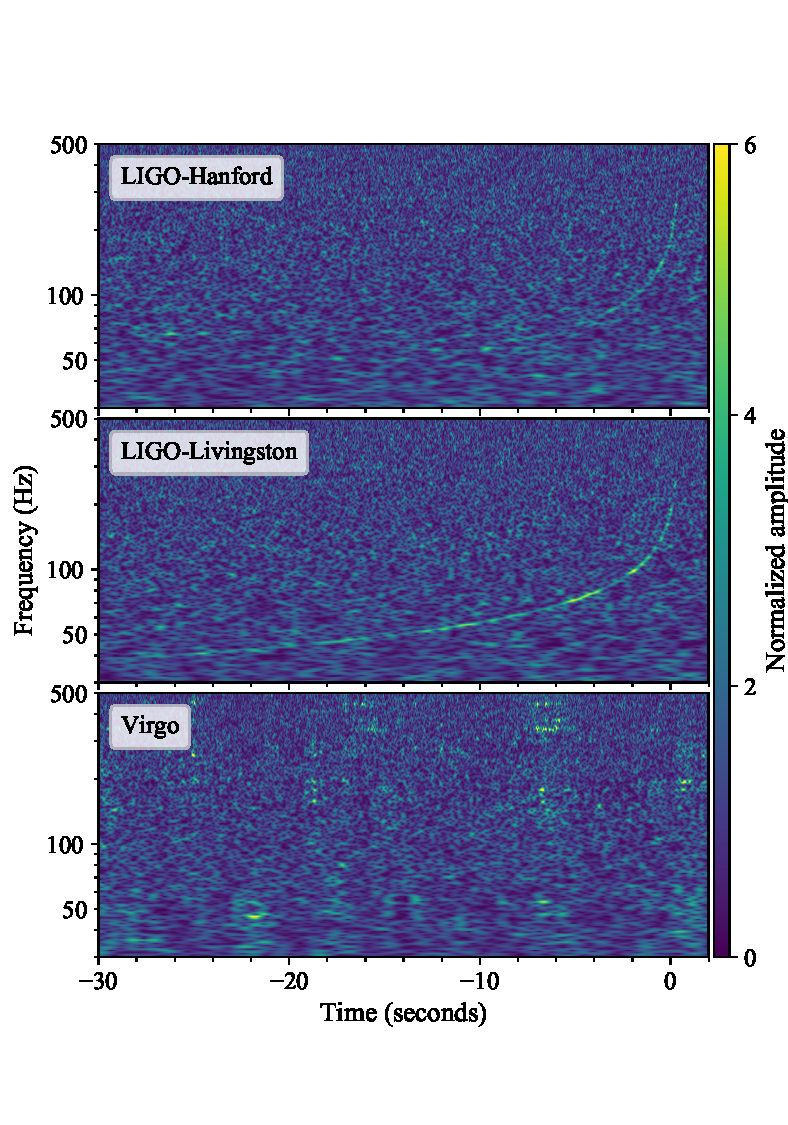
\includegraphics[width=0.8\textwidth]{GW170817.pdf}
\caption[Spectrogram of the strain caused by a binary neutron star merger]{Spectrogram of the strain caused by a binary neutron star merger as seen at the LIGO Hanford Observatory, LIGO Livingston Observatory, and the Virgo Observatory. \cite{GW170817} A clear chirp signal can be seen starting at $\sim$40 Hz which rises in both frequency and amplitude. The origin of the time axis is the time at which the neutron stars merge. The differing amount of signal in the three detectors is due to the alignment of their respective antenna-patterns with the source location.}
\label{GW170817}
\end{center}
\end{figure}
 
 Although binary systems are the topic of choice here, many other systems should theoretically emit gravitational waves. These can range from asymmetric spinning stars \cite{contGW} and supernovae \cite{SN} to cosmic strings \cite{strings} and density perturbations in the early universe \cite{inflation}. With the measurement of gravitational waves, humankind has technologically expanded our senses to include the faint vibrations of space-time. This ability has allowed the study of new types of astronomical systems and may one day allow further insight into the beginning of the universe and the nature of gravity.
\pagebreak
\section{LIGO}

\subsection{Sensitivity}

The Laser Interferometric Gravitational wave Observatory (LIGO) \cite{aLIGO} is a pair of 4-km-long L-shaped interferometric gravitational wave detectors, one located in Hanford, Washington (LHO) and the other in Livingston, Louisiana (LLO). Each observatory is a dual-recycled Fabry-Perot Michelson interferometer which measures the differential strain between its two arms formed by pairs of partially reflective mirrors, also called test masses. 
\begin{figure}[!h]
\begin{center}
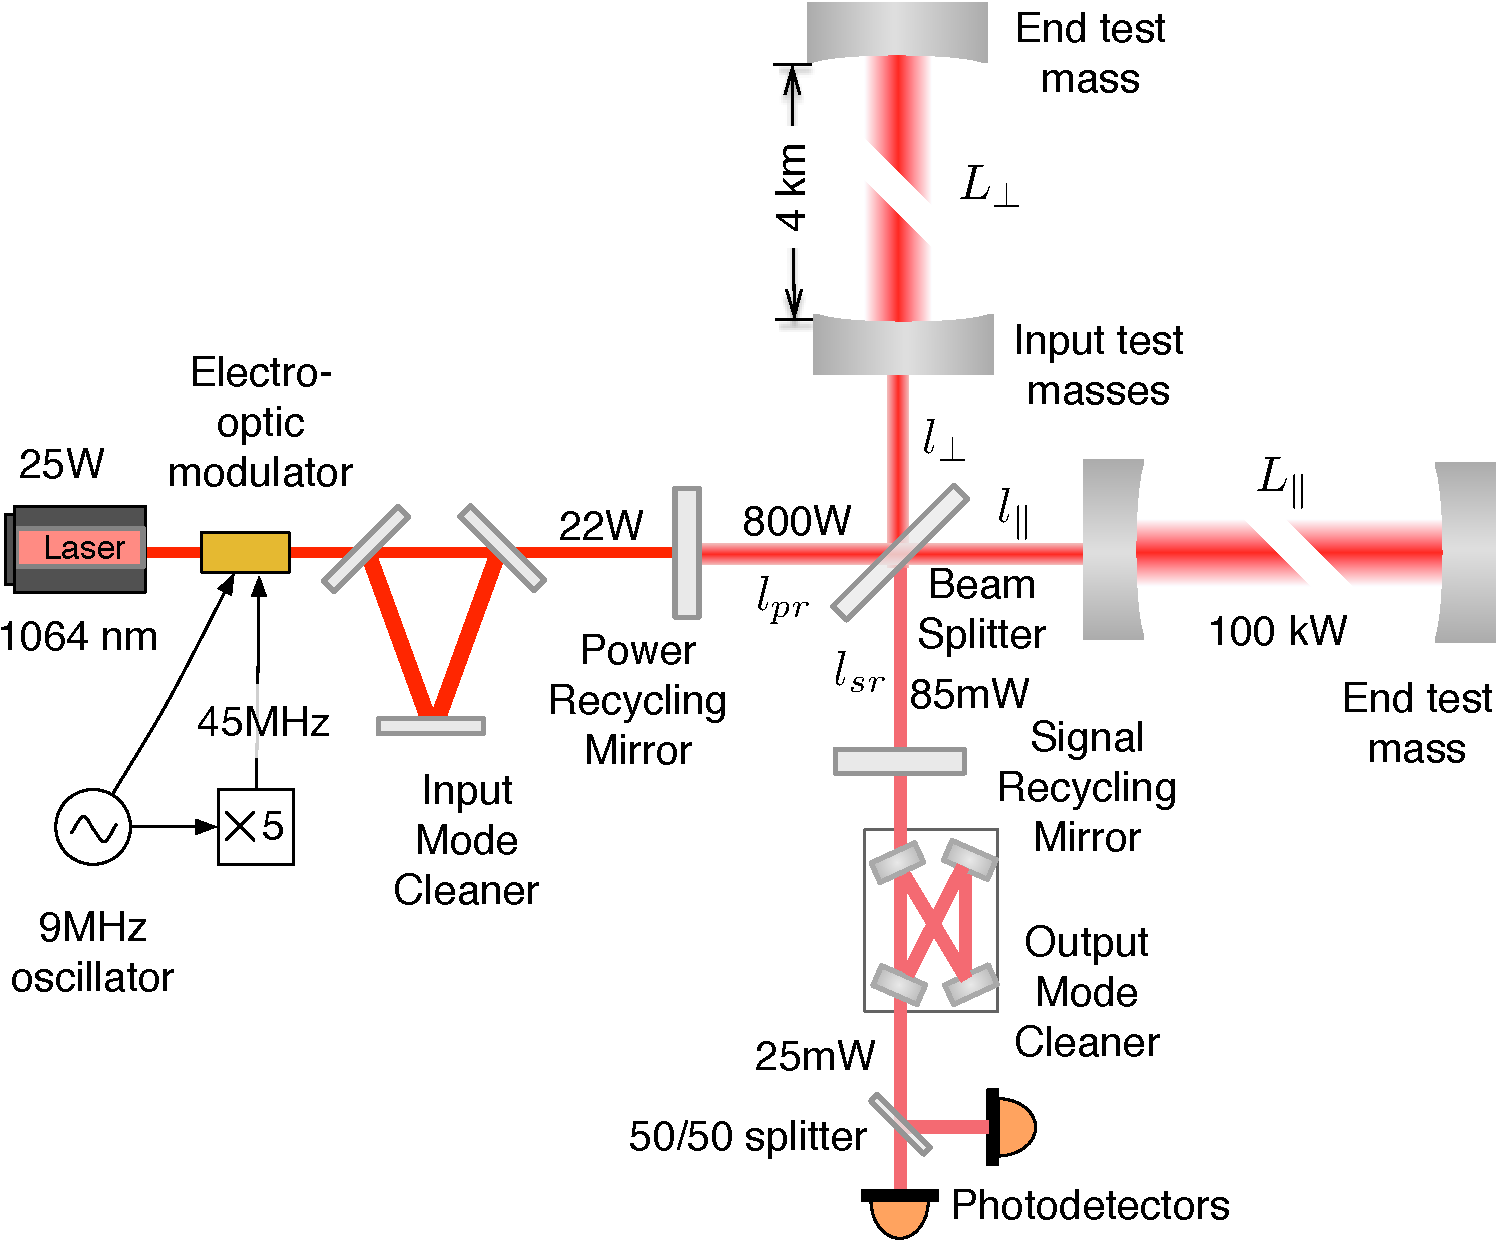
\includegraphics[width=0.75\textwidth]{LIGO_Schematic.pdf}
\caption[Optical layout of the LIGO interferometers]{Optical layout of the LIGO interferometers. Reprinted figure with permission from \cite{LIGOSens}. Copyright 2016 by the American Physical Society.}
\label{LIGO_Schematic}
\end{center}
\end{figure}

\pagebreak
As a gravitational wave passes the observatory, the arms experience strains that follow~\cite{GWBook}:
\begin{align}
h_{xx}&=h_+\ \big( \cos^2\theta\ \cos^2\phi-\sin^2\phi \big)+2\ h_\times\ \cos \theta\ \sin \phi \cos \phi \\
h_{yy}&=h_+\ \big( \cos^2\theta\ \sin^2\phi-\cos^2\phi \big)-2\ h_\times\ \cos \theta\ \sin \phi \cos \phi \\
\nonumber \\
h&=\frac{1}{2} \big( h_{xx}-h_{yy} \big)=\frac{1}{2}h_+\ \big( 1+\cos^2\theta \big)+ h_\times\ \cos \theta\ \sin 2 \phi 
\end{align}
where $h_{xx}$ and $h_{yy}$ are the strains along the x and y arms respectively, $\theta$ and $\phi$ are the polar and azimuthal angles of the direction of propogation, and $h$ is the differential strain as measured by the observatory. Here the polarizations are defined in the source frame.

The series of optics allows the observatory to measure differential strains down to $7\times10^{-24}$ at 200 Hz.  Noise curves for the observatories are shown in Figure \ref{LIGO_Strain} where one can see that the sensitive band of the observatory runs from 20 Hz up to 7 kHz. At low frequencies the noise is dominated by residual control noise, discussed in Section \ref{ASC}, while at high it is dominated by noise caused by quantum fluctuations.  \cite{Squeeze}

\begin{figure}[!h]
\begin{center}
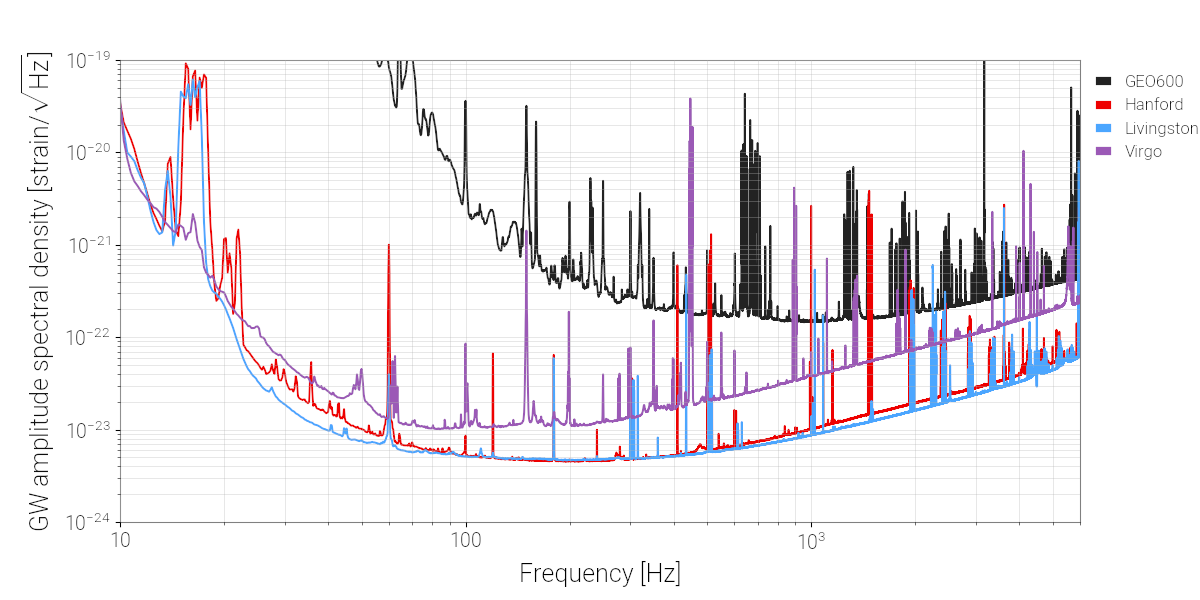
\includegraphics[width=\textwidth]{LIGOSens.png}
\caption[Strain sensitivity of the LIGO and Virgo Observatories]{Strain sensitivity of the LIGO Observatories during the third observing run. Also shown are the sensitivities of the Virgo and GEO600 observatories. \cite{LIGOopen}}
\label{LIGO_Strain}
\end{center}
\end{figure}


\subsection{Events}

With LIGO's current sensitivity, the primary systems of interest are compact binaries, discussed in Section \ref{CBC}, which merge within the band of interest. A equal mass $50\ M_\odot$ binary black hole system would merge at $\sim$22 Hz while a $1.4\ M_\odot$ binary neutron star system merges at $\sim$800 Hz yet emits appreciably while sweeping through the LIGO band.

During the first and second observing runs of LIGO, ten binary black hole systems and one binary neutron star merger were detected with high significance. \cite{GWTC} The black hole binaries ranged in total mass from $18.6\ M_\odot$ to $84.4\ M_\odot$ and merged at distances from 320 Mpc to 2.8~Gpc. The neutron star binary had component-masses of $1.27\ M_\odot$ and $1.46\ M_\odot$ and merged at 40 Mpc. These systems are tabulated in Table \ref{gwTable}.

\begin{center}
\begin{tabular}{| c | c | c | c | c | c |}
\hline
Event Name & m1 ($M_\odot$) & m2 ($M_\odot$) & $M_f\ (M_\odot)$ & Distance (Mpc) & z\\
\hline \hline
GW150914 & $35.6^{+4.7}_{-3.1}$ & $30.6^{+3.0}_{-4.4}$ & $63.1^{+3.4}_{-3.0}$ & $440^{+150}_{-170}$ & $0.09^{+0.03}_{-0.03}$\\
\hline
GW151012 & $23.2^{+14.9}_{-5.5}$ & $13.6^{+4.1}_{-4.8}$  & $35.6^{+10.8}_{-3.8}$ & $1080^{+550}_{-490}$& $0.21^{+0.09}_{-0.09}$\\
\hline
GW151226 & $13.7^{+8.8}_{-3.2}$ & $7.7^{+2.2}_{-2.5}$ & $20.5^{+6.4}_{-1.5}$ & $450^{+180}_{-190}$ & $0.09^{+0.04}_{-0.04}$\\
\hline
\hline
GW170104 & $30.8^{+7.3}_{-5.6}$ & $20.0^{+4.9}_{-4.6}$ & $48.9^{+5.1}_{-4.0}$ & $990^{+440}_{-430}$ & $0.20^{+0.08}_{-0.08}$\\
\hline
GW170608 & $11.0^{+5.5}_{-1.7}$ & $7.6^{+1.4}_{-2.2}$ & $17.8^{+3.4}_{-0.7}$ & $320^{+120}_{-110}$ & $0.07^{+0.02}_{-0.02}$\\
\hline
GW170729 & $50.2^{+16.2}_{-10.2}$ & $34.0^{+9.1}_{-11.1}$ & $79.5^{+14.7}_{-10.2}$ & $2840^{+1400}_{-1360}$ & $0.49^{+0.19}_{-0.21}$\\
\hline
GW170809 & $35.0^{+8.3}_{-5.9}$ & $23.8^{+5.1}_{-5.2}$ & $56.3^{+5.2}_{-3.8}$ & $1030^{+320}_{-390}$ & $0.20^{+0.05}_{-0.07}$\\
\hline
GW170814 & $30.6^{+5.6}_{-3.0}$ & $25.2^{+2.8}_{-4.0}$ & $53.2^{+3.2}_{-2.4}$ & $600^{+150}_{-220}$ & $0.12^{+0.03}_{-0.04}$\\
\hline
GW170817 & $1.46^{+0.12}_{-0.10}$ & $1.27^{+0.09}_{-0.09}$ & $\le2.8$ & $40^{+7}_{-15}$ & $0.01^{+0.00}_{-0.00}$\\
\hline
GW170818 & $35.4^{+7.5}_{-4.7}$ & $26.7^{+4.3}_{-5.2}$ & $59.4^{+4.9}_{-4.8}$ & $1060^{+420}_{-380}$ & $0.21^{+0.07}_{-0.07}$\\
\hline
GW170823 & $39.5^{+11.2}_{-6.7}$ & $29.0^{+6.7}_{-7.8}$ & $65.4^{+10.1}_{-7.4}$ & $1940^{+970}_{-900}$ & $0.35^{+0.15}_{-0.15}$\\
\hline
\hline
GW190412 & $29.7^{+5.0}_{-5.3}$ & $8.4^{+1.7}_{-1.0}$ & $37.0^{+4.1}_{-3.9}$ & $730^{+140}_{-170}$ & $0.15^{+0.03}_{-0.03}$\\
\hline
GW190425 & $1.60-1.87$ & $1.46-1.69$ & $3.4^{+0.3}_{-0.1}$ & $159^{+69}_{-71}$ & $0.03^{+0.01}_{-0.02}$\\
\hline
\end{tabular}
\label{gwTable}
\end{center}

The recently completed third observing run has had 56 significant candidates \cite{O3events}. Although these candidates have not been verified to be true gravitational wave events, they show a significant increase in rate of detection due to both the decreased noise and increased duty cycle achieved for the third observing run. Two of these candidates have been confirmed to be true gravitational wave events: GW190412 \cite{GW190412} a binary black hole merger with asymmetric component-masses and GW190425 \cite{GW190425} a binary merger with total mass of $\sim$~3.4~$M_\odot$

Observation of gravitational waves has led to further understanding of a variety of phenomena including the nature of the neutron star composition \cite{NSEoS}, the source of heavy elements \cite{heavyElements}, and black hole populations \cite{GWTC}. Additionally, they have allowed a model independent measurement of Hubble's constant \cite{hubble1, hubble2} and have set restrictive constraints on alternative theories of gravity \cite{speedGW}.

\section{Seismic Isolation}\label{seisIso}

\subsection{LIGO Isolation Scheme}

To operate interferometric observatories that are sensitive to the strains of space-time, one must isolate the instrument from all other sources of differential displacement. As the observatories are located on the surface of the earth, the dominant source of such noise is ambient seismic motion. 

The ambient seismic wave-field, measurements of which are shown in Figure \ref{groundSpec}, is continuously excited across a wide frequency range. Between 50 mHz and 1 Hz the ambient spectrum is dominated by the ``microseism'', an always-present feature sourced by the Earth's oceans. Above 1 Hz, the dominant source of seismic motion at the observatories is due to local activity. Yet even in locations without anthropogenic sources, the ground moves at these frequencies. Without isolation, this motion would dominate any measurements with the interferometer and, more practically, would disrupt any attempt to operate the interferometer at its ideal alignment. This ideal alignment is referred to as having the interferometer ``locked''.

\begin{figure}[!h]
\begin{center}
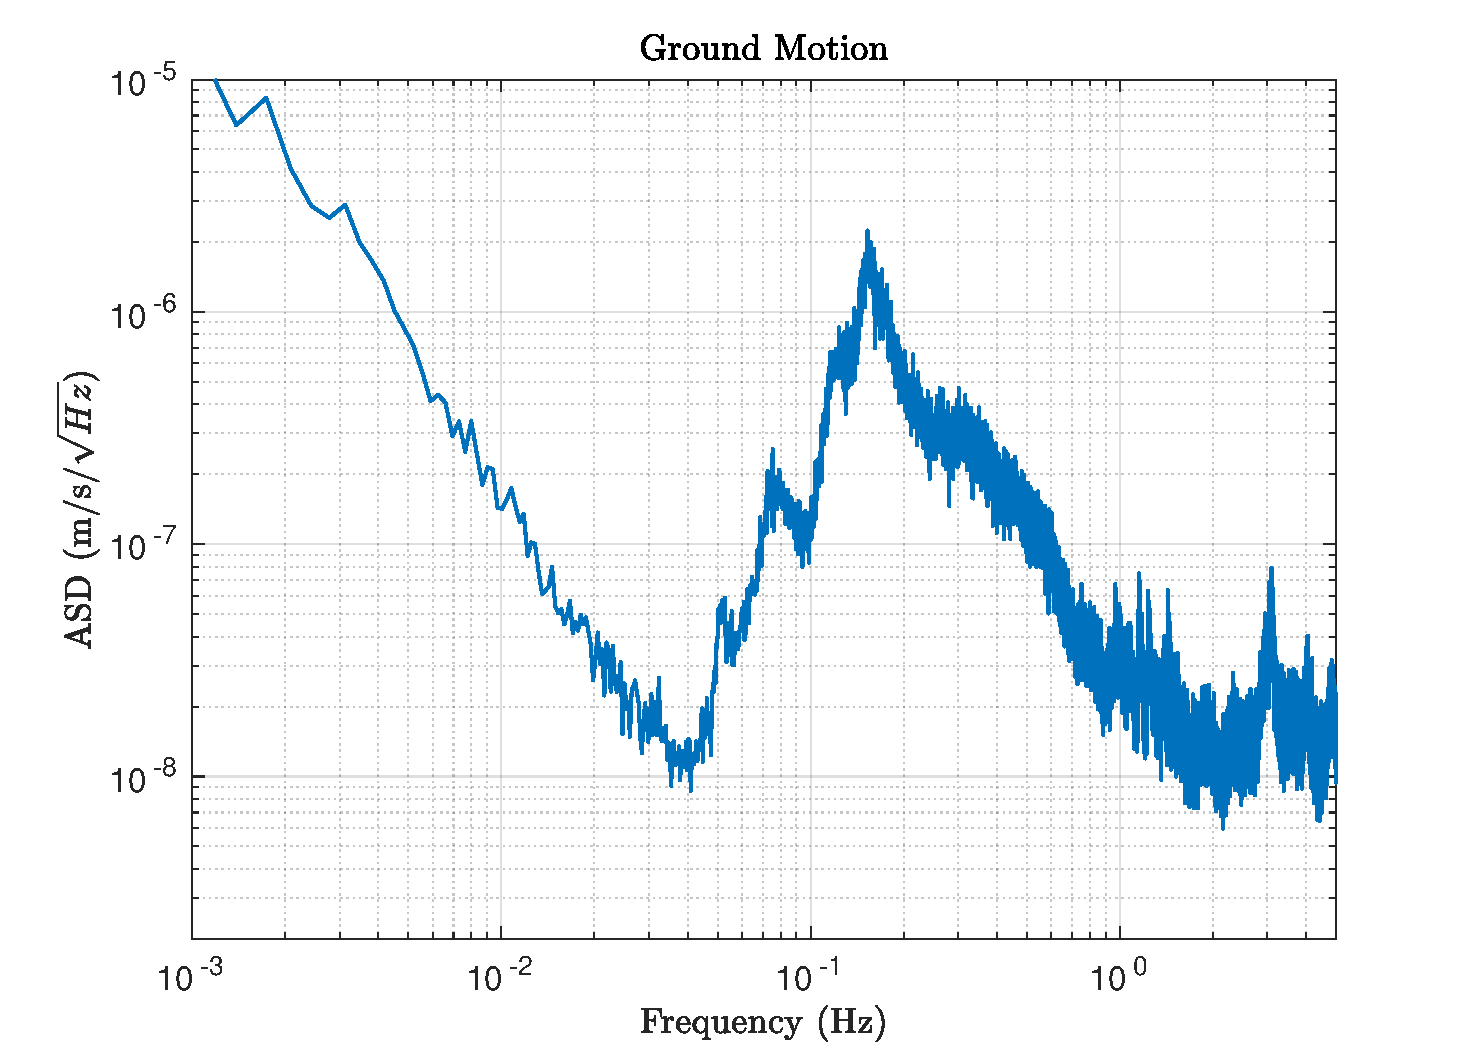
\includegraphics[width=0.85\textwidth]{GroundSpectrum.pdf}
\caption[Example ambient ground motion spectrum]{Example ambient horizontal ground motion spectrum recorded at the End-X station of the LIGO Hanford Observatory. From 40 mHz to 1 Hz the spectrum is dominated by the oceanic microseism while above 1 Hz the seismic motion is sourced by local anthropogenic activity. Below 40 mHz, the instrument is dominated by tilt contamination described in Section \ref{tiltCon}}
\label{groundSpec}
\end{center}
\end{figure}

The LIGO observatories solve this issue by employing a multi-stage seismic isolation system formed of both passive and active stages. \cite{ligoSeis} First from the ground is the Hydraulic External Pre-Isolation (HEPI) system which is formed by four hydraulic actuators. This provides a factor of $\sim$100 isolation at high frequencies and allows for correction of tidal effects. Suspended from this is the Internal Seismic Isolation (ISI) system\footnote{LIGO employs two versions of the ISI: the HAM-ISI for the auxiliary optics and the BSC-ISI for the core optics. Here ISI refers to the BSC-ISI as rotation sensors have only been deployed on BSC-ISIs.}, described in Section \ref{ISI}. This is a dual-stage six-degree active isolation system and is the primary broad-band isolation. From the second stage of the ISI is hung a quadruple pendulum, at the bottom of which is a test mass. This provides high frequency passive isolation that attenuates the motion of the test mass by $1/f^8$, where $f$ is the frequency of the motion.

\begin{figure}[!h]
\begin{center}
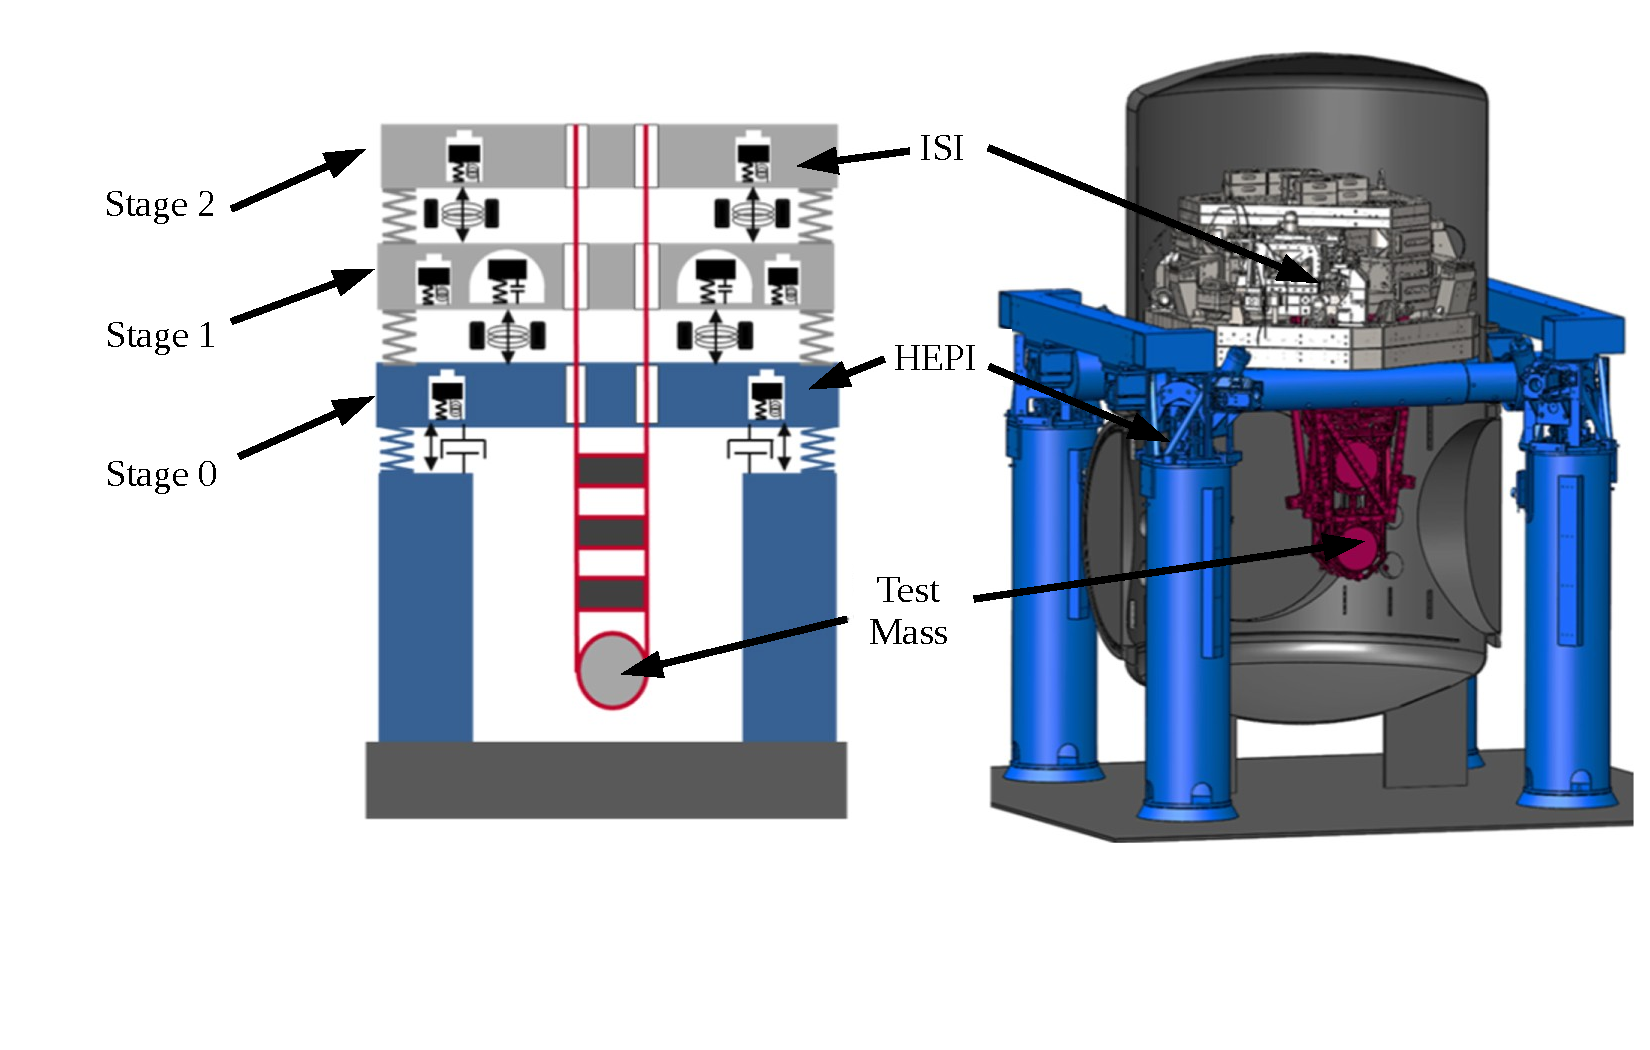
\includegraphics[width=\textwidth]{seismicIso.pdf}
\caption[Schematic of the LIGO seismic isolation system]{Schematic of the LIGO seismic isolation system. \cite{ligoSeis} On the left is a cartoon showing the three stages of isolation while on the right is a CAD rendering of the seismic isolation system and vacuum chamber.}
\label{wind}
\end{center}
\end{figure}

\subsection{Internal Seismic Isolation}\label{ISI}

The ISI is comprised of two similar stages each suspended from steel blade springs and wires. The first (Stage 1) is suspended from HEPI (Stage 0) and the second (Stage 2) from the first. Each stage is controlled by a set of six magnetic actuators whose feedback signal is comprised of a collection of sensors. The motion of the table is sensed with a series of seismometers which are sensitive to motion with respect to an inertial frame. On the first stage, two separate models of seismometers are combined to obtain the lowest noise in a given frequency band. Sarcelles L4Cs are used above 0.5 Hz, while below this Trillium T240s are employed. These two sensors are ``blended'' together by sending the T240 through a low pass filter and the L4C through a high pass. The filtered signals are added together to form a low-noise broad-brand inertial sensor combination. The second-stage utilizes Geotech GS13s as its inertial sensors.

The inertial motion of the platform is sensed in all six degrees of freedom using three independent seismometers of each type located 1-meter apart. The three translational signals are composed from the average of the corresponding seismometer signals, while the three rotational degrees are sensed using the difference of the motion divided by the separation.

\begin{figure}[!h]
\begin{center}
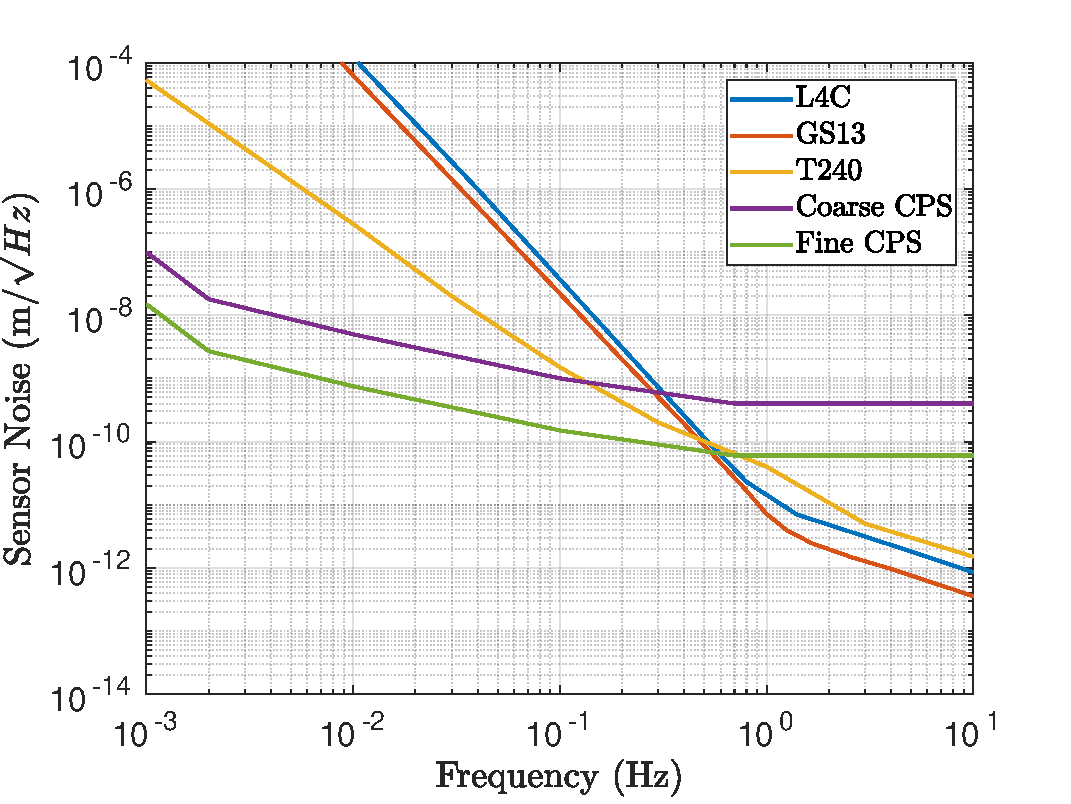
\includegraphics[width=0.85\textwidth]{seismicSensNoise.pdf}
\caption[Sensor noise for the seismic isolation system]{Sensor noise for the collection of sensors used on the ISI. The L4C, GS13, and T240 are seismometers while the Coarse CPS and Fine CPS are position sensors. The isolation system blends the relevant sensors together to achieve the lowest possible noise.}
\label{seisNoise}
\end{center}
\end{figure}

Due to the increased T240 noise below 500 mHz, a set of Capacitive Position Sensors (CPS) are deployed to detect the relative motion between either Stage 0 and the first ISI stage or the two stages of the ISI. This is then used as the control signal at low frequencies yielding a control for Stage 1 that follows:

\begin{equation}
x_\text{cont}=F_{LP}\ (x_\text{p}-x_\text{g})_\text{,CPS}+F_{BP}\ x_\text{p, T240}+F_{HP}\ x_\text{p, GS13}
\end{equation}

where $x_\text{cont}$ is the control signal, $x_\text{p,i}$ is the platform motion sensed by the respective sensor, $x_\text{g}$ is the ground motion, and $F_\text{LP},\  F_\text{BP},\ F_\text{HP}$ are respectively a low-pass, band-pass, and high-pass filter. When this signal is utilized in feedback, the residual motion of the platform can be approximated by:
\begin{equation}
x_p(f)\approx F_{LP}\ \big(x_g(f)+n_\text{CPS}(f)\big)+F_{BP}\ n_\text{T240}(f)+F_{HP}\ n_\text{GS13}(f)
\end{equation}

where $n_{i}(f)$ is the sensor noise spectrum for the relevant sensor. This approximation ignores tilt-to-horizontal coupling which is addressed in Section \ref{tilt}.

\subsection{Sensor Correction}\label{SensCor}

The isolation can be further improved with the addition of a three-axis seismometer, in this case a Struckheisen STS-2, placed on the floor of the observatory. This measures the ground motion and can be used to do ``sensor correction''. Sensor correction is the procedure of subtracting the ground contribution of the CPS signal to recover the low frequency platform motion. The CPS signal in this case becomes:
\begin{equation}
x_{CPS}=F_{LP}\ (x_p-x_g)+F_{SC}\ x_g
\end{equation}

where $F_{SC}$ is the ``sensor correction'' filter which has a pass-band that overlaps the CPS low pass filter. This can be rearranged to give:
\begin{equation}
x_{CPS}=\tilde F_{LP}\ (x_p-x_g)+\tilde F_{HP}\ x_p
\end{equation}

where the tildes denote the relevant combination of $F_{LP}$ and $F_{SC}$ that yield effective low-pass and high-pass filters. This scheme allows for isolation down to 100 mHz and decreases the bleed-through of the  ground motion due to the CPS low-pass filter's finite roll-off. Below 10 mHz, both the ground and platform seismometers are dominated by tilt contamination which is addressed in Section \ref{tilt}. The performance of the seismic isolation system can be seen in Figure \ref{ISIPerf}.

\begin{figure}[!h]
\begin{center}
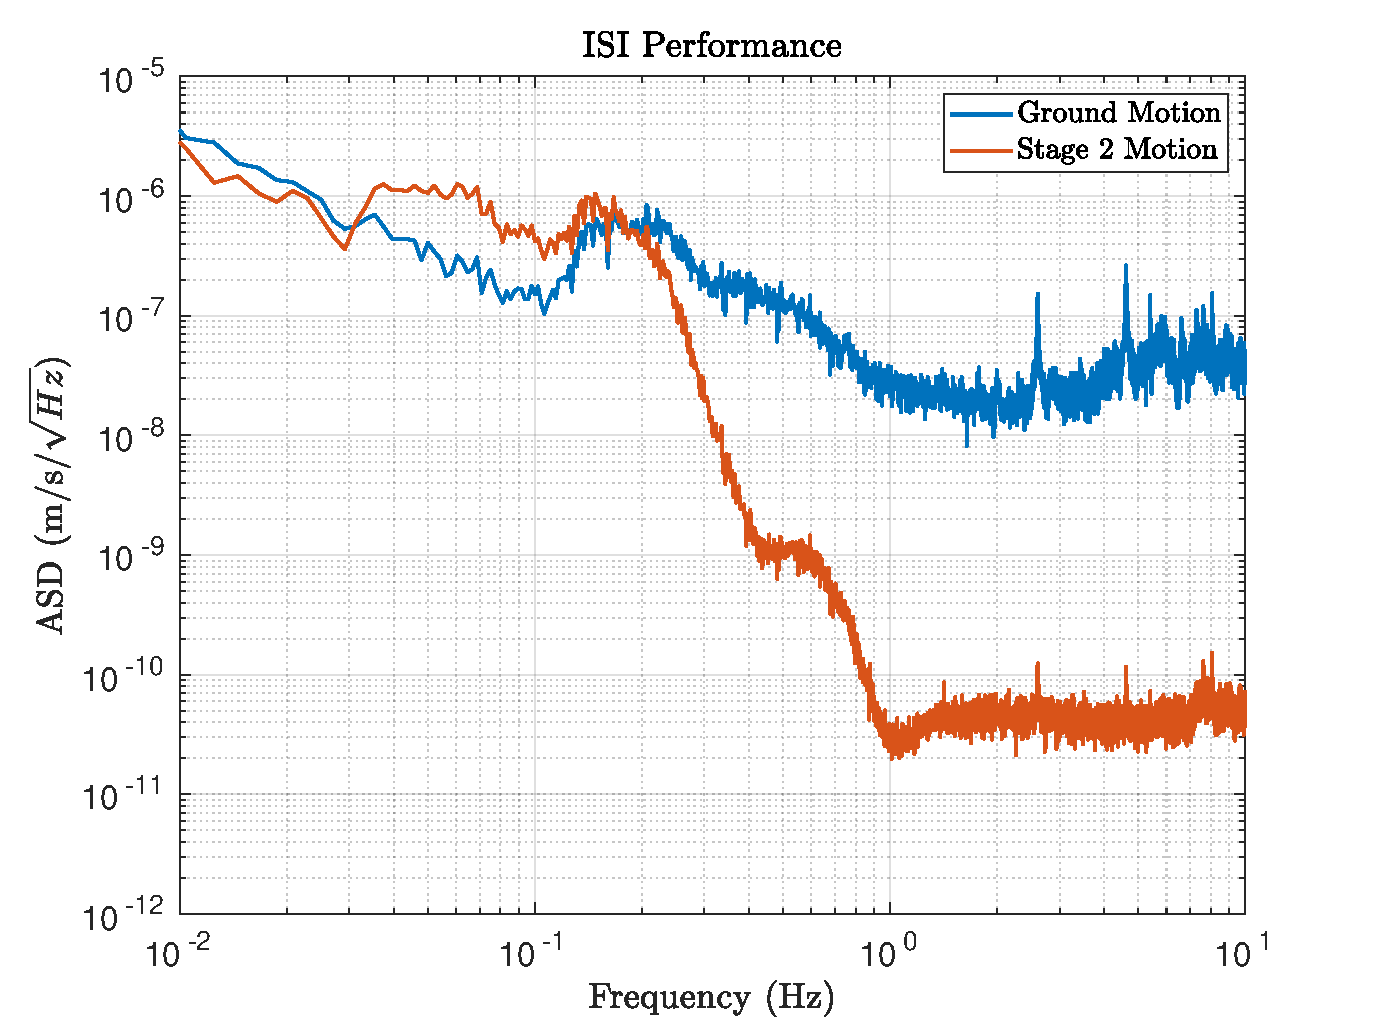
\includegraphics[width=\textwidth]{ISIPerf.pdf}
\caption[Performance of the ISI]{Performance of the ISI as measured by the GS13 installed on Stage 2. A factor of $\sim$1000 reduction in motion is achieved above 1 Hz. Below which sensor noise and residual ground motion limit the performance.}
\label{ISIPerf}
\end{center}
\end{figure}

\chapter{1-meter Scale Ground Rotation Sensors} \label{BRS_chap}
\section{Ground Tilt}\label{tilt}
\subsection{Tilt Contamination}\label{tiltCon}
\quad At their core, seismometers are low frequency spring-mass systems that measure the difference in motion between the casing and the device's proof mass. Above the resonant frequency of the spring-mass system, this difference measures the motion of the casing with respect to an inertial frame. Over the past century this technology has produced devices that are sensitive to $\sim$0.1 nm/s down to $\sim$10 mHz. However, these systems are intrinsically susceptible to any stray forces that act on the proof mass.

Of interest here is the contamination due to the rotation of the device within a external gravitational field, namely the field caused by the Earth. The rotation with respect to a fixed gravitational force will be referred to as ``tilt''.\footnote{Although a subtle difference, the distinction would be of great consequence if the local gravitational field were to vary rapidly. In that case the sensors described in Sections \ref{BRSSec} and \ref{cBRSSec} would be of little use as the sense inertial rotations not tilts with respect to gravity.} From the proof mass's frame, a tilt is equivalent to a rotation of the gravitational force. This yields a horizontal acceleration of:
\[ a=g \sin(\theta)\]
where $g$ is the gravitational acceleration on the surface of the earth and $\theta$ is the angle by which the device is tilted. This acceleration adds a second term to the seismometer's output shown below for small angles and in the Fourier domain:
\[\tilde{x}_{seis}(\omega)=\tilde{x}_{trans}(\omega)+\frac{g}{\omega^2}\tilde{\theta}(\omega)\]
where $\tilde{x}_{seis}$ is the seismometer's output in displacement units, $\tilde{x}_{trans}$ is the translational motion of the device, and $\omega$ is the angular frequency. 

With this additional contribution, it is clear that, for a given amplitude of tilt, the contamination term contributes more at lower frequencies and can readily dominate the translational signal. In the context of the ground seismometers at the observatory, the tilt signal exceeds the translational component below $\sim$100 mHz. Above this frequency, the seismometer signal is dominated by the ever-present oceanic microseism. This can be seen in Figure \ref{wind} which shows the translation amplitude spectral density measured by a ground seismometer at LHO during both low and high wind conditions.

\begin{figure}[!h]
\begin{center}
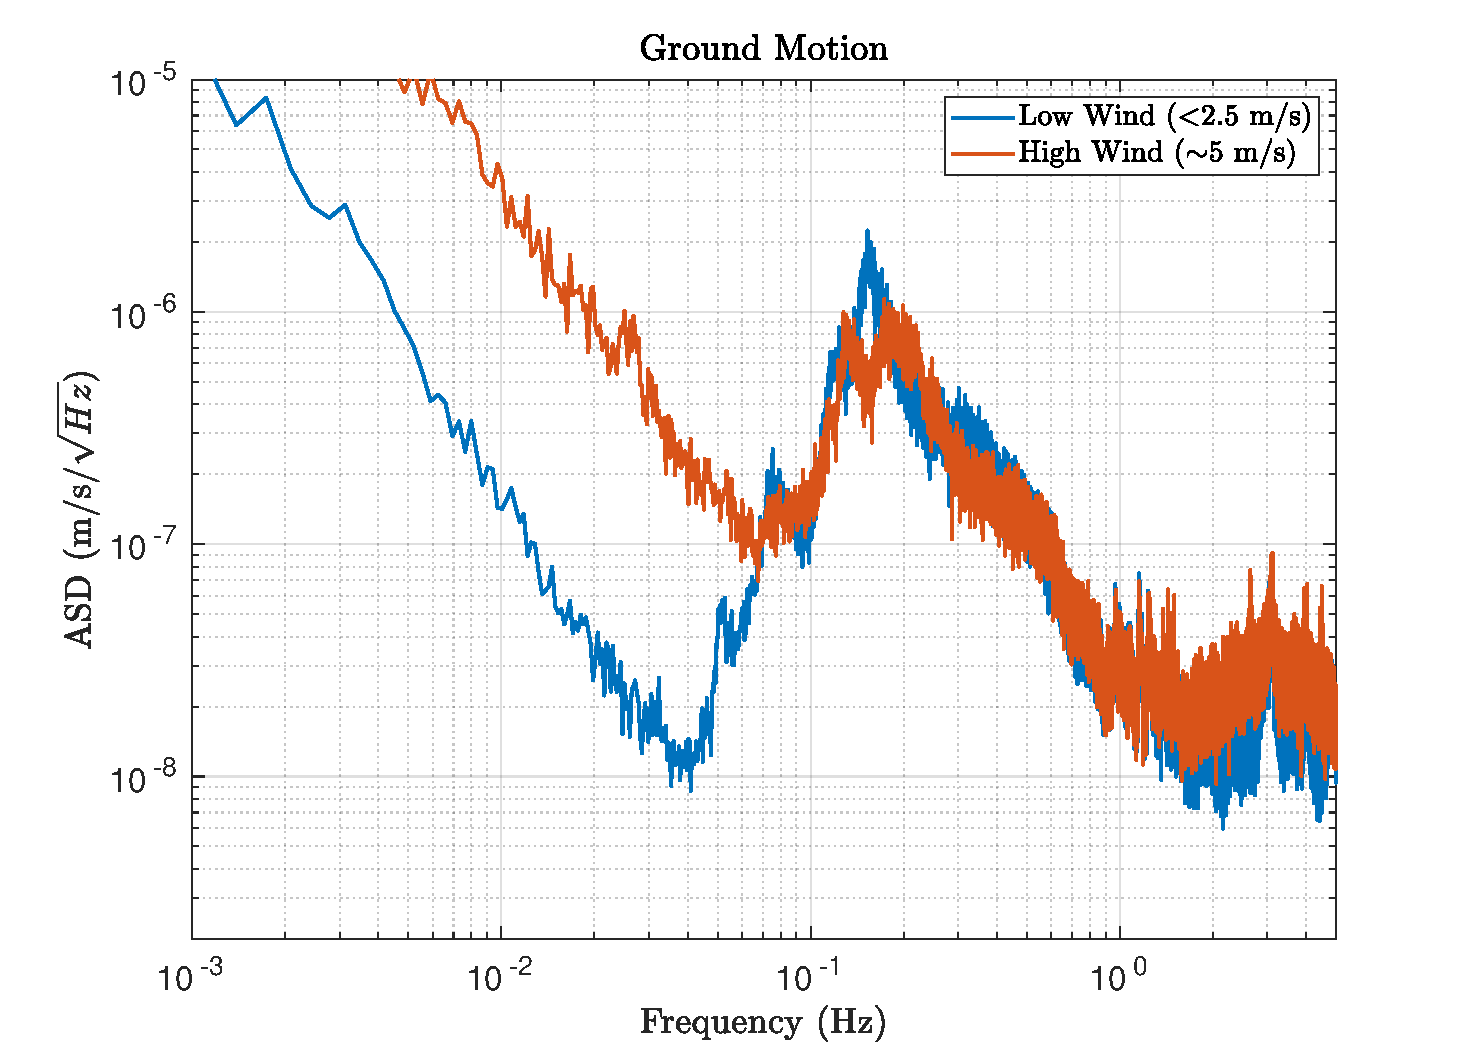
\includegraphics[width=0.85\textwidth]{windComp2.pdf}
\caption[Ground motion spectra during low and high winds]{Ground motion spectra recorded at the X-End Station of the Hanford Observatory during low and high winds. Below 100 mHz, wind driven tilts become dominant during high winds. From 100 mHz to 1 Hz the spectra are dominated by the oceanic microseism while above 1 Hz the seismic motion is sourced by local anthropogenic activity.}
\label{wind}
\end{center}
\end{figure}

The dominant driver of ground tilts at the observatories is wind acting on the walls of the building. Although one might naively assume that the wind would rigidly rotate the building, the true mechanism is deformation of the concrete slab caused by differential pressure on the walls of the building. This increases the noise seen by the ground seimometer during high winds. The primary consequence of this excess is that the interferometer could not remain locked during high wind speeds. Additionally, due to nonlinear deformation of the floor, tilts measured in one location can not be simply extrapolated from the tilts measured at a different location.

\subsection{Sensor Correction with Tilt Subtraction}

\quad Several different scheme, in principle, can combat such a contamination. The most straight-forward is to decrease the effect of wind by designing buildings that interact with the wind less or by installing wind blocks such as wind fences or earthen berms. Both of these options require significant construction and, for the case of LIGO, tilt contamination was not addressed in the observatories construction. Another option is to build seismometers that are suspended in such a way that they do not experience tilts. This is an active area of research and may one day yield tilt-free seismometers. \cite{tiltFree}

The approach that will be explored here is to measure the tilt with an independent inertial rotation sensor, described in Section \ref{BRSSec}, and subtract the wind-driven contribution. This would then yield a corrected channel with the following form:
\begin{align}
\tilde{x}_{seis}(\omega)=\tilde{x}_{trans}(\omega)+&\frac{g}{\omega^2}\tilde{\theta}(\omega)\\
-&\frac{g}{\omega^2}\tilde{\theta}_{meas}(\omega)
\end{align}

where $\tilde{\theta}_{meas}$ is the tilt seen by the rotation sensor. Given a subtraction factor of $\alpha$ between the tilt component of the seismometer and rotation sensors this yields the following:

\[\tilde{x}_{seis}(\omega)=\tilde{x}_{trans}(\omega)+\frac{g}{\omega^2}(1-\alpha)\tilde{\theta}(\omega)\]

Current installations have yielded an $\alpha\sim 0.9$. This yields a ground motion measurement with low tilt contamination which can be used within the seismic isolation system. As this correction decreases noise primarily at low frequencies, the feedback filters deployed within the isolation system can be tuned to cross over at a lower frequency away from the microseism. At the cross-over frequency, the filters have large gain and phase changes that degrade performance. Placing this cross-over below the microseism frequencies decreases the effects of this ``gain peaking'' and allows for isolation at lower frequencies. For more details see Reference \cite{windproofing}.

\section{Beam Rotation Sensors} \label{BRSSec}
\subsection{Mechanical System}

\quad A Beam Rotation Sensor (BRS) is a beam-balance based inertial rotation sensor comprised of a 1-m long aluminum beam suspended by two 10-15 $\mu$m-thick beryllium-copper flexures. Details of the flexure design can be found in Section \ref{flex}. The beam has a 1.7-kg brass mass attached to each end. This increases the moment of inertia to $I=0.51\text{ kg m}^2$. Figure \ref{BRSImage} shows a CAD model of the beam-balance. 

\begin{figure}
\begin{center} 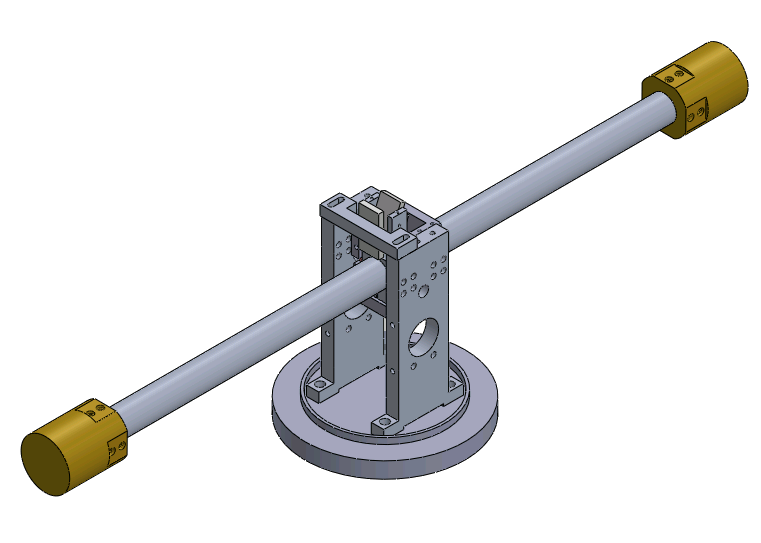
\includegraphics[width=0.75\textwidth]{BRSIso.png}
\caption[CAD rendering of the BRS]{CAD rendering of the BRS with the vacuum and optical readout systems omitted. The beam with its two brass end masses can be seen along with its attached mirrors and support structure. }
\end{center}
\end{figure} 
\begin{figure}
\begin{center} 
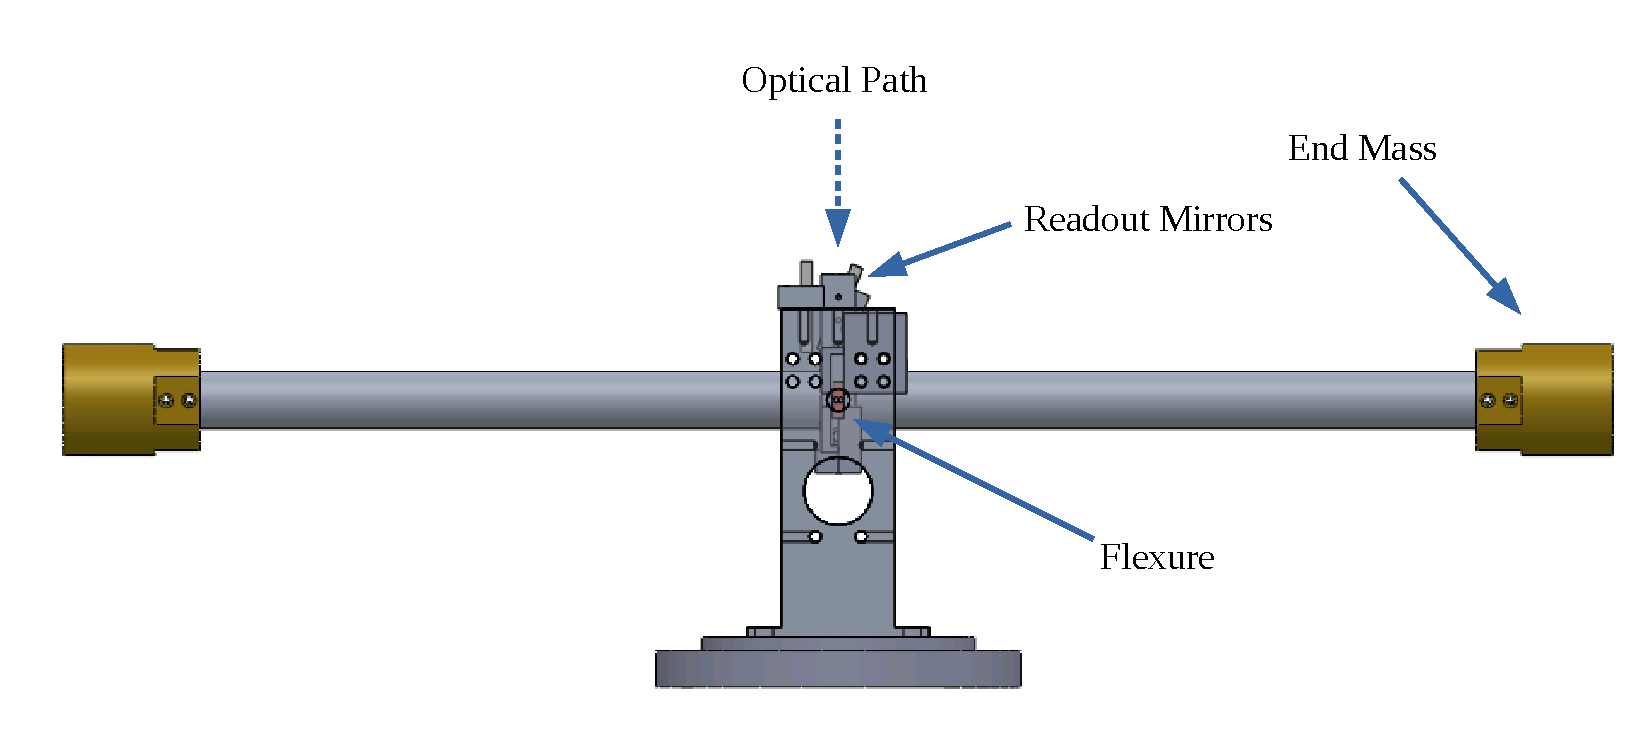
\includegraphics[width=0.95\textwidth]{BRSFrontLabeled.pdf}
\end{center}
\caption[Side view of a CAD rendering of the BRS]{Side view of a CAD rendering of the BRS. At center, one of the small copper-colored flexures can be seen. The other is mounted on the opposite side.}
\label{BRSImage}
\end{figure}


The balance is stiff in all degrees of freedom except rotation about the horizontal axis that intersects the two pivot-points. The BRS can be describes as a system consisting of two elementary subsystems: a rotational spring-mass system formed by the torsional stiffness of the flexures, and a simple gravitational pendulum due to the offset between the pivot point and the beam's center of mass. IT is then described by the following equation of motion: \cite{venk2014}

\begin{equation}
I \ddot{\theta}+ \gamma \dot{\theta}+\kappa (1+ \frac{i}{Q})(\theta-\theta_p)+M g \delta \theta +M \delta \ddot{x_p}=\tau_{ex} \label{eom}
\end{equation}

where $\theta$ and $\theta_p$ are, respectively, the angles of the beam and the platform with respect to gravitational vertical, $\tau_{ex}$ is the sum of all exterior torques, $I$ is the beam's moment of inertia, $Q$ is the intrinsic quality factor, $\gamma$ is the velocity damping factor, $\kappa$ is the spring constant of the flexures, $M$ is the mass of the balance, $g$ is the gravitational acceleration, $\delta$ is the vertical distance from the center of mass and the pivot point, and $x_p$ is the translation of the platform. Equation \ref{eom} can be rearranged to yield:

\begin{equation}
\tilde{\theta} = -\frac{\tilde{\tau}_{ex}+\omega^2 M \delta \tilde{x}_p+\kappa (1+i/Q) \tilde{\theta}_p}{I\omega^2-i \gamma \omega -i \kappa /Q-\kappa -Mg\delta}
\end{equation}

where $\omega$ is the angular frequency of motion and tildes denote spectral amplitudes. For the BRS, the measured quantity is not the angle of the beam but the difference in angle between the beam and the platform. Thus the angle recorded by the readout, $\theta_a$, follows:

\begin{align}
\tilde{\theta}_a &=\tilde{\theta}-\tilde{\theta}_p\\
&= -\frac{\tilde{\tau}_{ex}+\omega^2 M \delta \tilde{x}_p- (I\omega^2-i\gamma \omega -Mg\delta) \tilde{\theta}_p}{I\omega^2-i \gamma \omega -i \kappa /Q-\kappa -Mg\delta}
\end{align}
This equation can be broken into three distinct terms: the angular motion due to external torques, $\theta_\tau$, due to translational coupling, $\theta_x$, and due to rotation of the platform, $\theta_s$.
\begin{align}
&\tilde{\theta}_a =\tilde{\theta}_\tau+\tilde{\theta}_x+\tilde{\theta}_{s} \label{theta_A} \\ 
&\tilde{\theta}_\tau= -\frac{\tilde{\tau}_{ex}}{I}\frac{1}{\omega^2-i (\omega_0 \omega/q+\omega_0^2/Q)-(\omega_0^2+\omega_g^2)}\\
&\tilde{\theta}_x= -\tilde{x}_p\frac{M\delta}{I} \frac{\omega^2}{\omega^2-i (\omega_0 \omega/q+\omega_0^2/Q)-(\omega_0^2+\omega_g^2)}\\
&\tilde{\theta}_{s}= -\tilde{\theta}_p\frac{\omega^2-i\omega_0 \omega/q-\omega_g^2}{\omega^2-i (\omega_0 \omega/q+\omega_0^2/Q)-(\omega_0^2+\omega_g^2)}\label{theta_s}
\end{align}

Where $\omega_0=\sqrt{k/I}$ is the resonant frequency, $\omega_g=\sqrt{M g \delta/I}$, and $q$ is the quality factor due to velocity damping. These equations show that the beam has a resonance at $\omega=\sqrt{\omega_0^2+\omega_g^2}$ and $\tilde{\theta}_s$ has a minimum at $\omega=\omega_g$. 


\begin{figure}[!h]
\begin{center}
 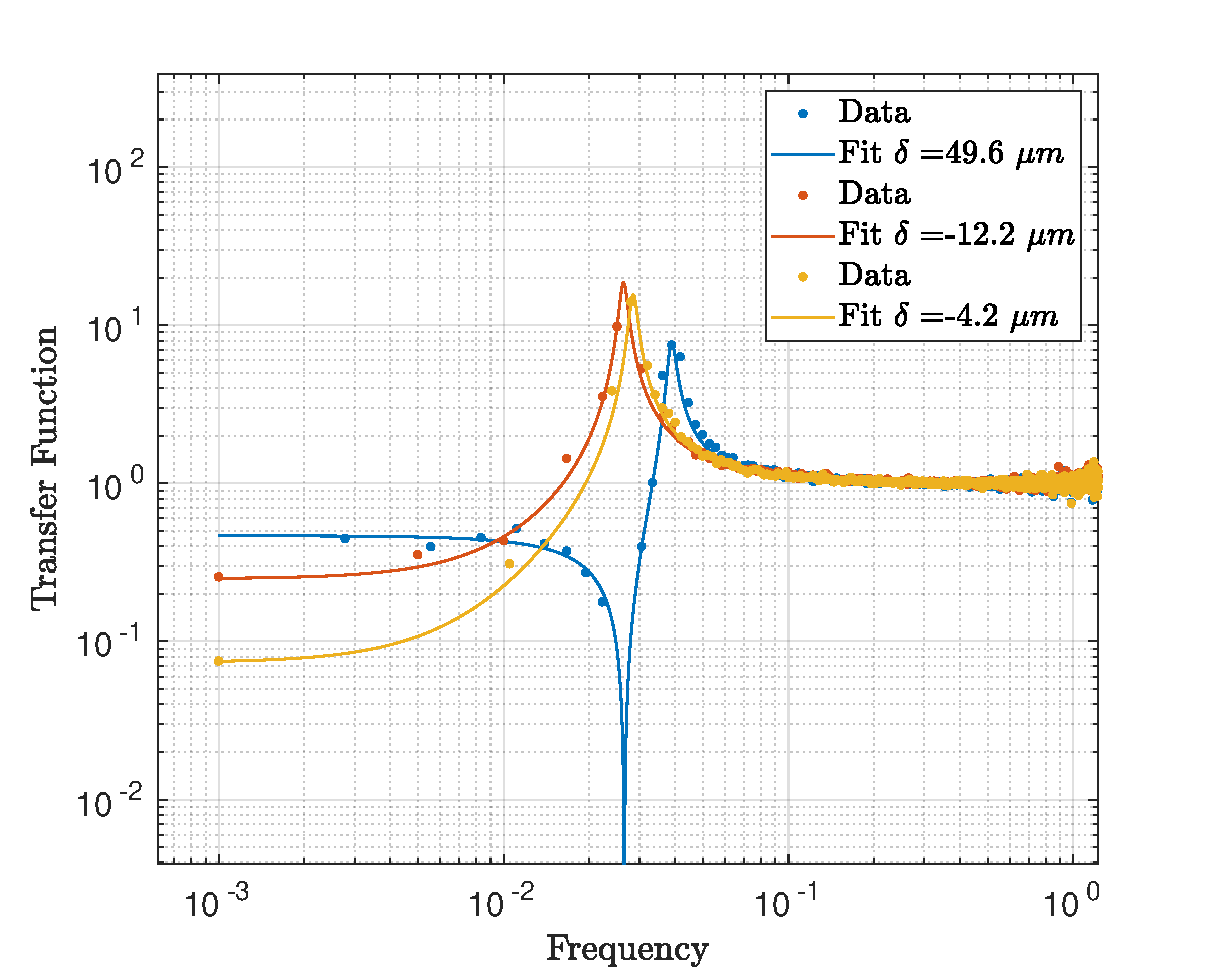
\includegraphics[width=0.85\textwidth]{cBRS_TransferFunction.pdf}
\caption[Transfer function from platform tilt to measured tilt for the cBRS]{Measurements of the transfer function from platform tilt to measured tilt for the compact-BRS, described in Chapter \ref{cBRS_chap}, along with fits to Equation \ref{theta_s}. After each measurement mass was added or removed from the top of the proof mass in order to shift the vertical position of its center of mass.}
\label{TransferFunction}
\end{center}
\end{figure}

To obtain high fidelity rotation sensing, the translational coupling must be negligible. To achieve this, the magnitude of $\delta$ must be minimized. This is achieved through the design of the beam's suspension which places the center of mass close to the pivot point. Fine adjustments are then made by adding mass to the beam above or below the pivot. These adjustments are guided by measurements of the $\tilde{\theta}_s$ transfer function, Equation \ref{theta_s}. Figure \ref{TransferFunction} shows this for the compact-BRS, described in Chapter \ref{cBRS_chap}. The amount of tuning that was achieved differed for each device deployed at the observatories due to scheduling constraints. The lowest translation coupling was achieved at the LHO End-Y BRS which had $\delta<0.5\ \mu$m yielding a translational coupling of $<10^{-6}$ rad/m.

\subsection{Flexures}\label{flex}

The flexures that suspend the proof mass are cut from $1/4''\times1/4''\times7/8''$ blocks of beryllium-copper by wire electrical-discharge machining to yield the shape shown in Figure \ref{flex}. Circular cuts were used to achieve a well-defined pivot point. The opening gaps on either side were restricted to act as mechanical stops for ease of handling and transportation.

Due to machining variation in the width of flexure, batches of flexures were assayed via a microscope to determine the width of each flexure and to identify flexures that were damaged during machining and transportation. Pairs of flexures with similar widths were installed together, one on each side of the beam. Each flexure has one half clamped to the support and the other attached to the beam, as shown in Figure \ref{BRSFrontD}. This provides a suspension which is stiff in all degrees of freedom except rotation about the axis intersecting the two pivot points. 

The stiffness of the flexure increases with thickness. The flexure width was minimized to decrease the resonant frequency of the beam balance. This was limited practically by the motion of the machining wire to yield flexures with widths of 10-15 $\mu$m. Although, flexures thinner than 10 $\mu$m could be achieved, the finished pieces contained irregular holes laterally through the flexure. These flexures would have lower breaking-strength and would degrade the performance if installed in a BRS. 

\begin{figure}[!h]
\begin{center}
 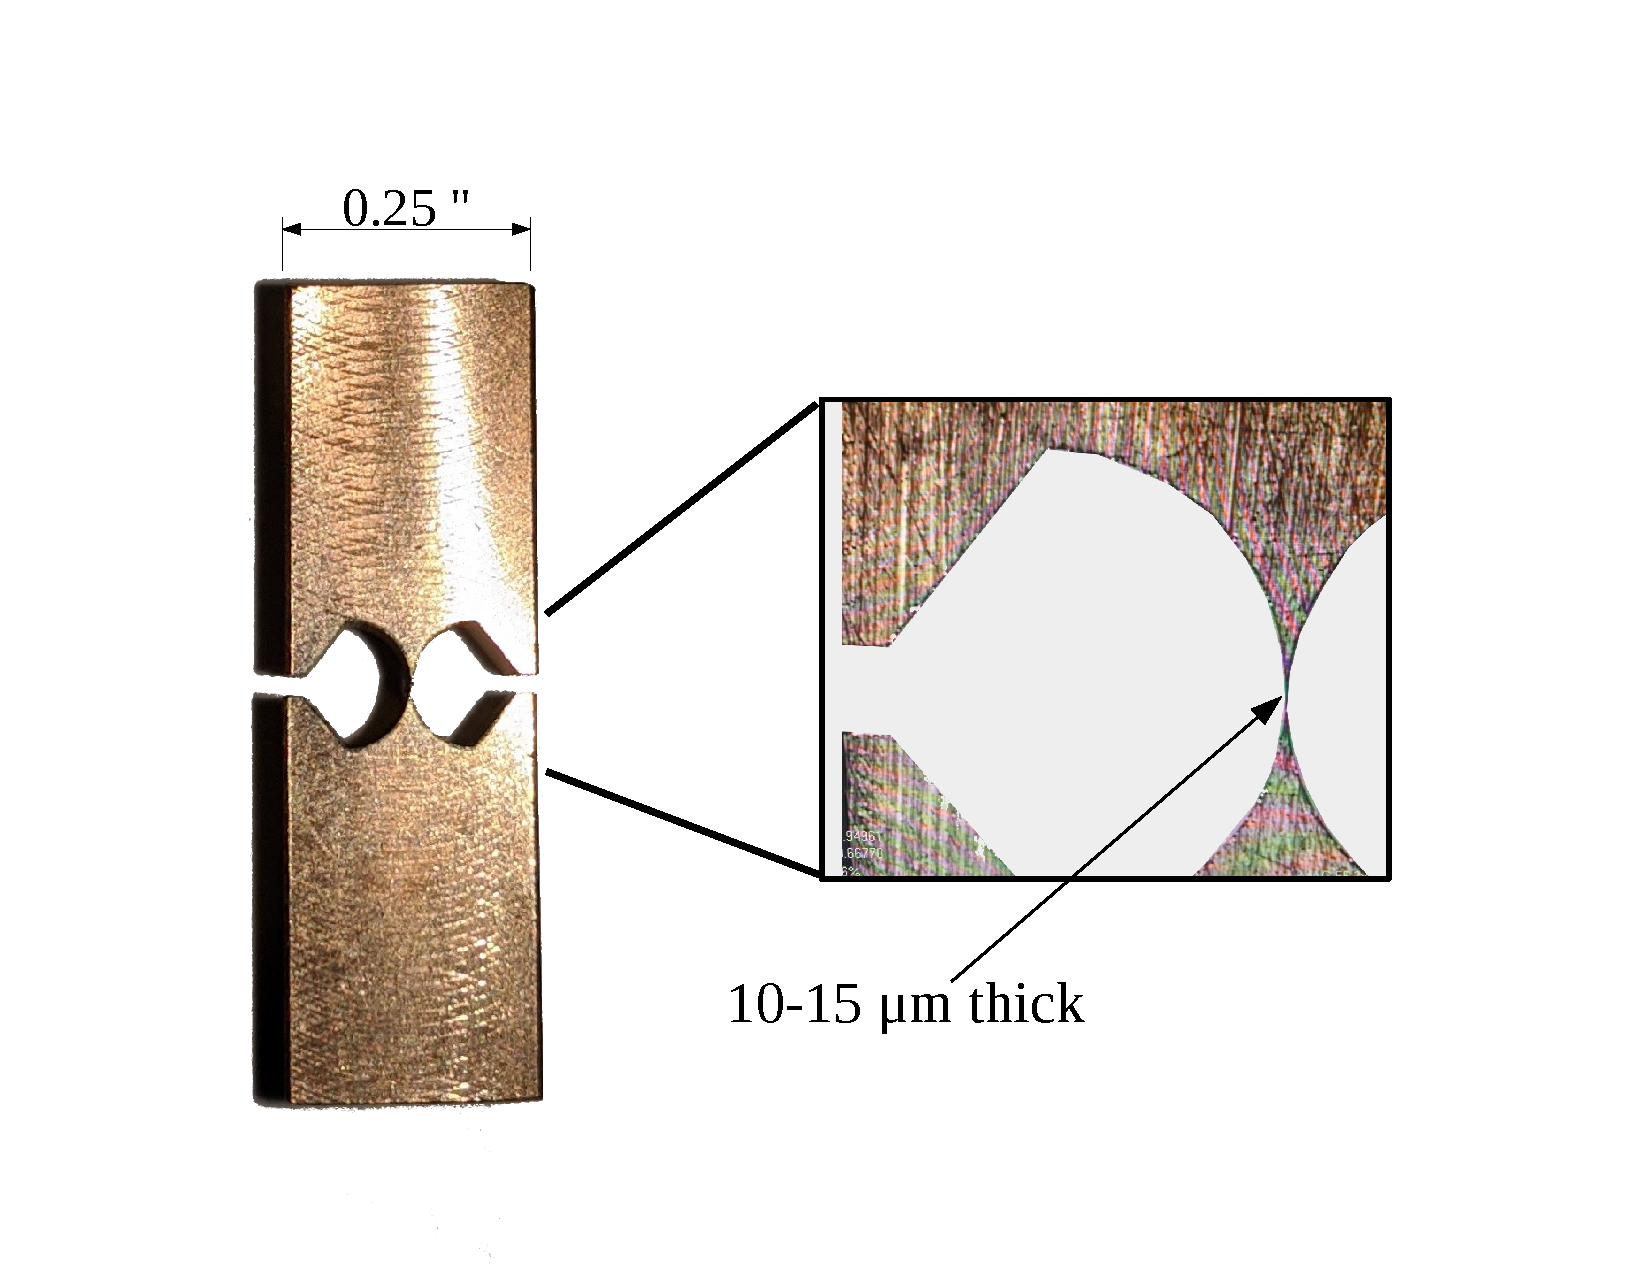
\includegraphics[width=0.75\textwidth]{Flexure.pdf}
\caption[Image of a BRS flexure]{Image of a flexure used to suspend the beam balance with detail showing microscope image of the flexure point.}
\label{flexure}
\end{center}
\end{figure}

\begin{figure}[!h]
\begin{center} 
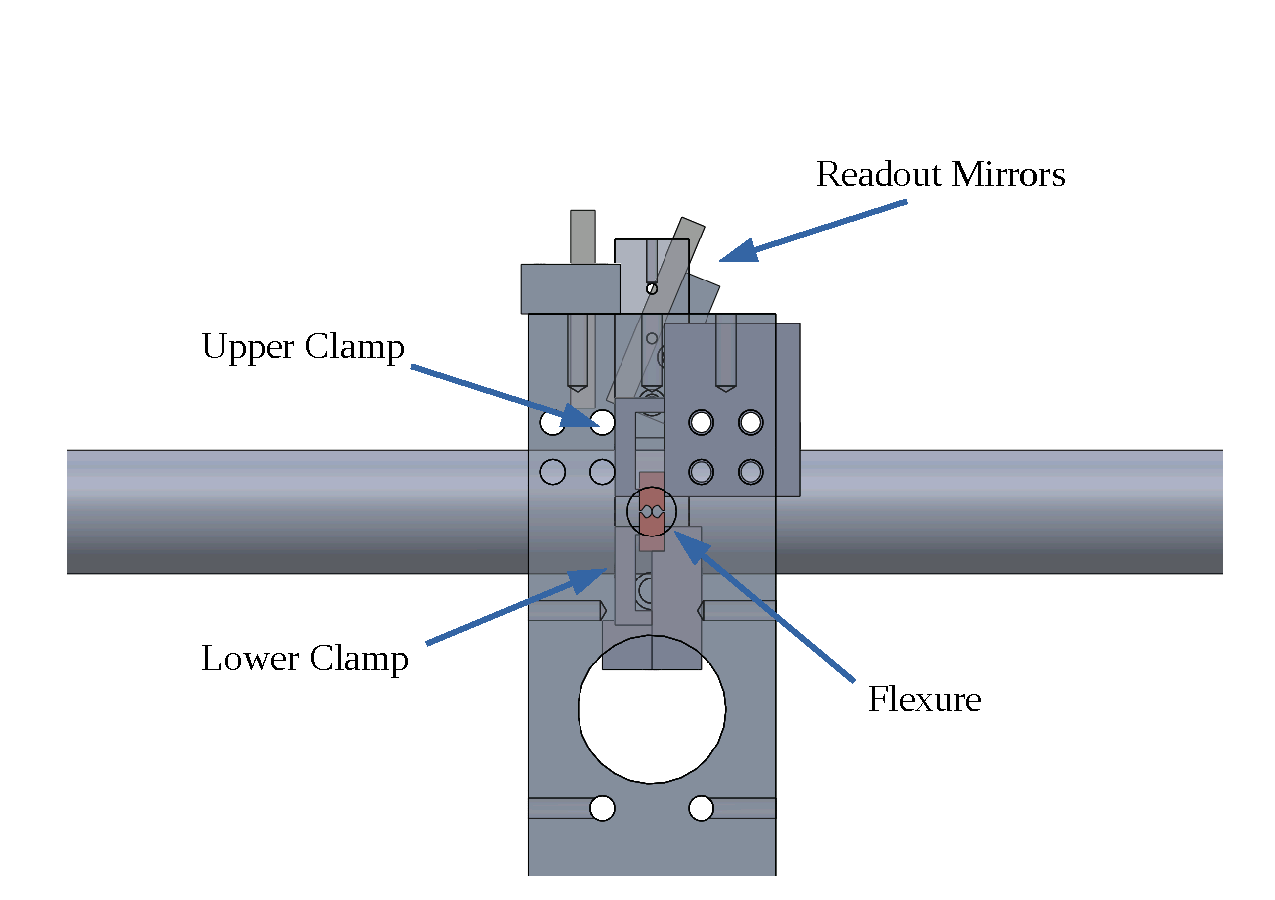
\includegraphics[width=\textwidth]{BRSFrontDetailLabeled.pdf}
\end{center}
\caption[Close up view of the center of the CAD rendering of the BRS]{Close-up view of the center of the CAD rendering of the BRS. One of the copper colored flexures can be seen at center along with its clamps. The two gray blocks at the top are mirrors for optical sensing, one fixed to the support the other attached to the beam.} \label{BRSFrontD}
\end{figure}

\subsection{Vacuum System}

To decrease the effects of air currents and gas damping, each BRS is placed into its own vacuum chamber that emulates the outline of the device, shown in Figure \ref{BRSPic}. This chamber is initially evacuated to $\sim \mu$Torr pressures using a roughing pump and turbomolecular pump. After which, the vacuum is maintained by a 10 l/s ion pump which further decreased the pressure to $\sim$0.1~$\mu$Torr.

\begin{figure}[!h]
\begin{center}
 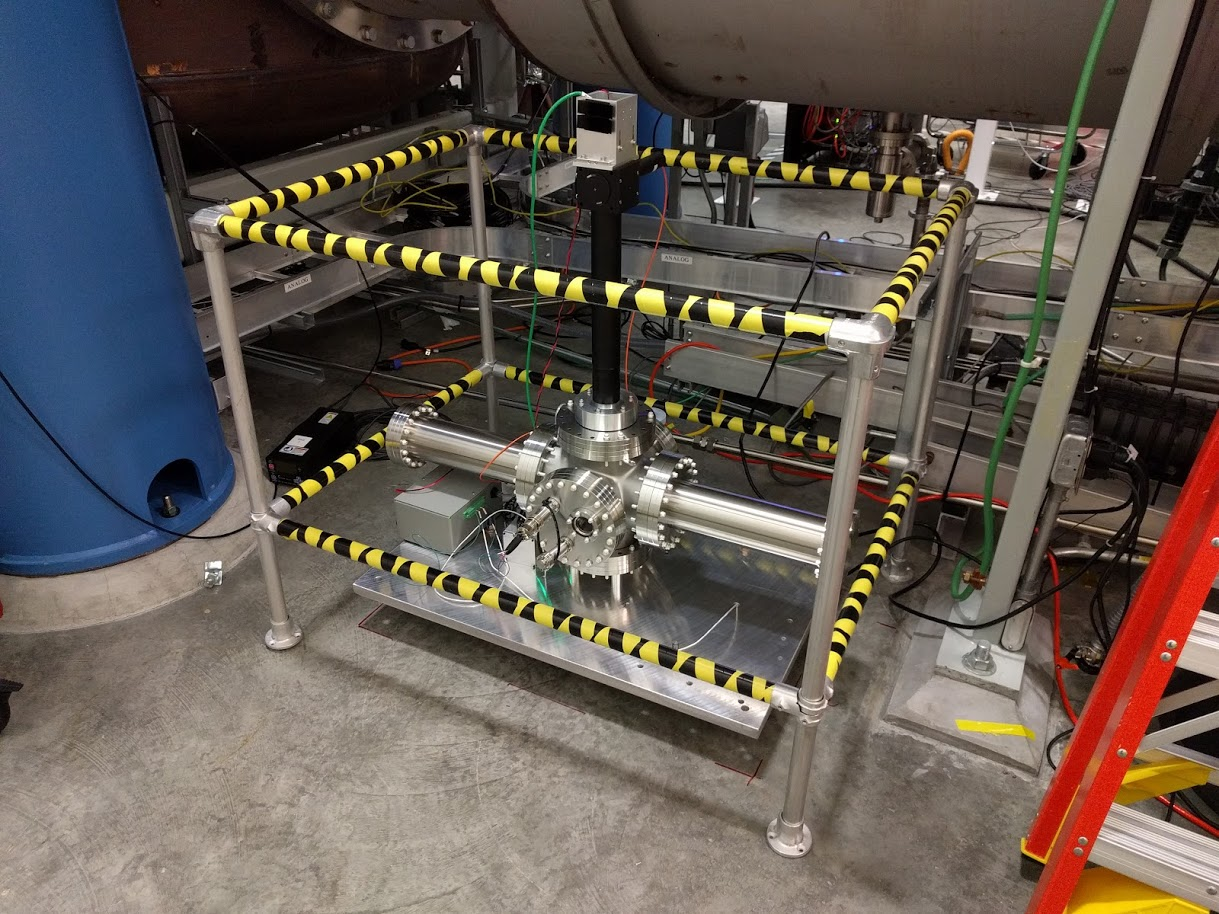
\includegraphics[width=\textwidth]{BRSPic.jpg}
\caption[Picture of an installed BRS]{Picture of the BRS installed at LIGO Livingston Observatory End-Y before the installation of the thermal insulation.}
\label{BRSPic}
\end{center}
\end{figure}

\subsection{Multi-Slit Autocollimator Readout}

The angular deflection is measured by a multi-slit autocollimator \cite{MSA} that can be viewed as an improved optical lever.

Optical levers are simple optical angular readouts that exploit the law of reflection to measure angular deflections of a mirror by observing the displacement of a reflected beam of light. The angle of the mirror is described as:
\begin{equation}
\theta_{s}=\frac{x_{\text{reflected}}}{2d}
\end{equation}
where $\theta_\text{mirror}$ is the angle of the mirror, $x_\text{reflected}$ is the displacement of the reflected beam, and $d$ is the distance between the optical system and the mirror. This allows one to increase the precious of the angular measurements arbitrarily by increasing $d$. However, with this comes the disadvantage that the effective gain of the sensor depends on $d$ which may not be well known and may vary in time.

An autocollimator \cite{MSA} adds a lens located one focal-length from both the light source and the detector. This effectively replaces the distance dependence with the focal length of the lens. Thus the system is sensitive only, to first order, to the angular motion of the mirror.

\begin{figure}%
\begin{center}
 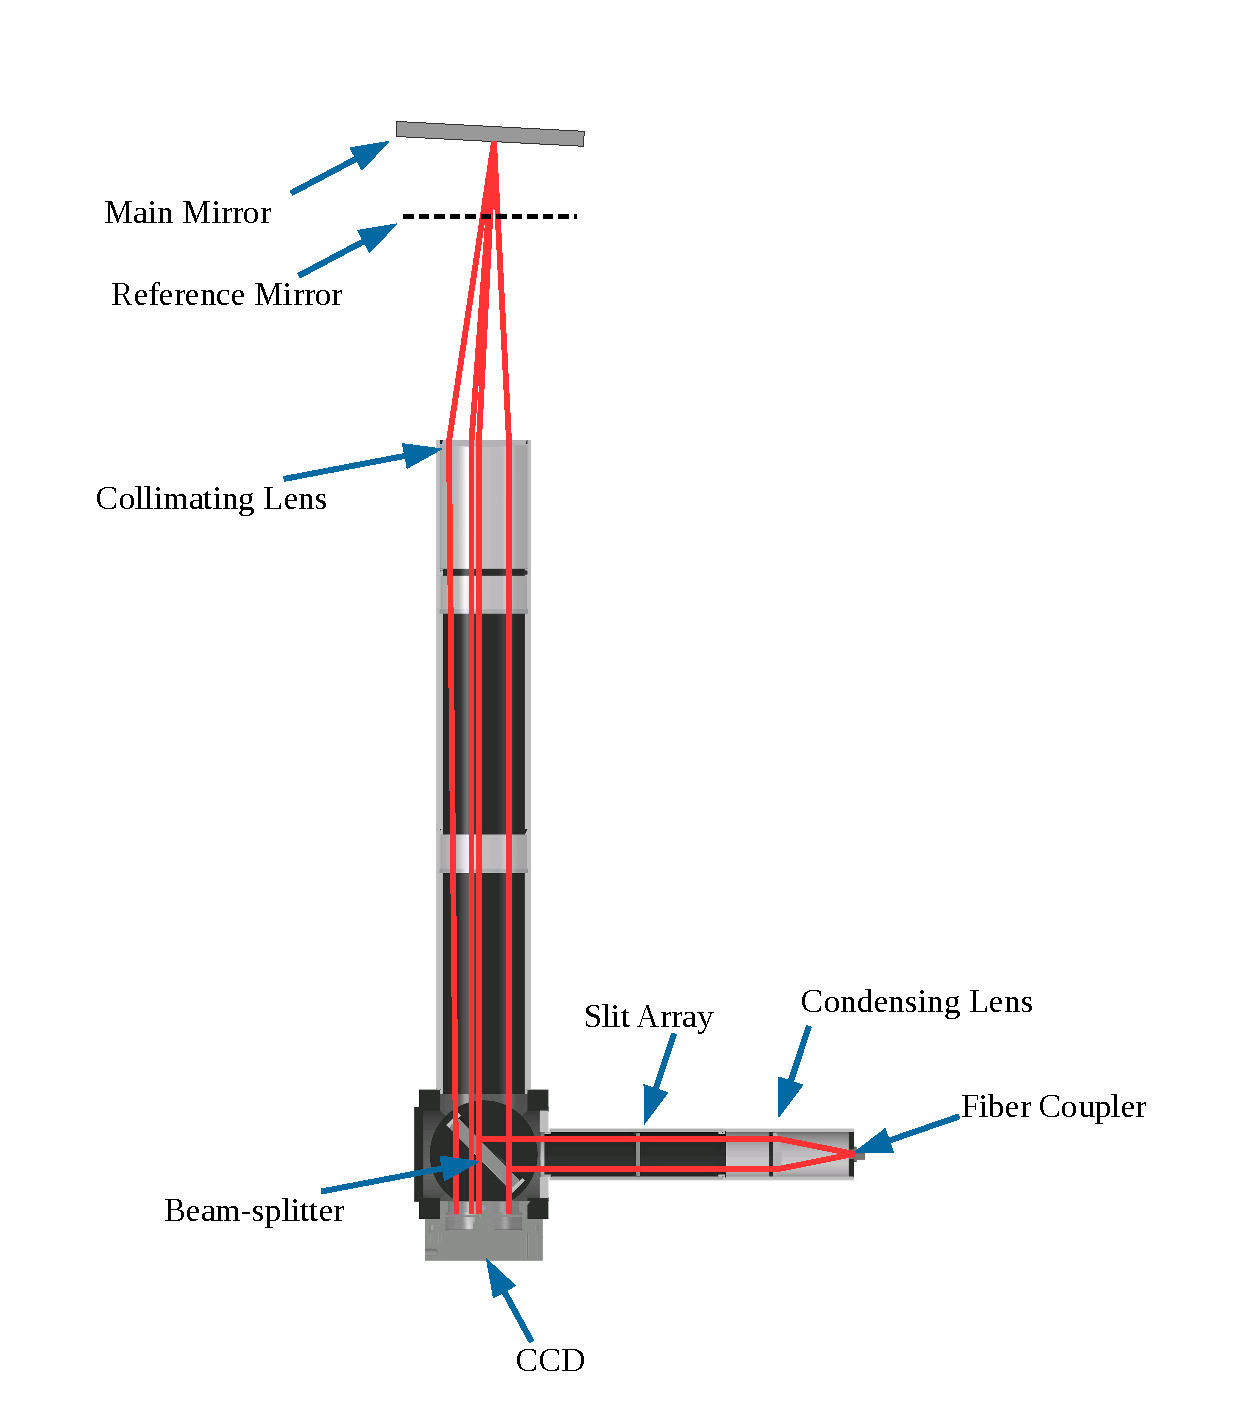
\includegraphics[width=\textwidth]{Autocollimator2.pdf}
\caption[Schematic of a multi-slit autocollimator]{Schematic of a multi-slit autocollimator used as the angular readout of the BRSs. The light enters through the fiber coupler, is collimated by the condensing lens, and images the slit array. This image is then partially reflected by the beam-splitter, focused onto the main mirror by the collimating lens, and returns through the collimating lens to be imaged on the CCD. A second pattern is made by the partial reflection off the reference mirror and is also imaged on the CCD.}
\label{ACFig}
\end{center}
\end{figure}

To improve this system further, a partially-reflective mirror can be placed in between the autocollimator and the main mirror to act as a reference. This allows for the subtraction of any perceived motion that is not due to motion of the main mirror. The angular readout is then described by:
\begin{equation}
\theta_{s}=\frac{x_{\text{main}}-x_{\text{reference}}}{2f}
\label{ACEq}
\end{equation}

where $f$ is the focal length of the lens and $x_\text{reference}$ is the location of the beam-spot from the reference mirror.

\begin{center}
\begin{tabular}{| c | c |}
\hline
Parameter & Value\\
\hline \hline
CCD & Balser Racer raL4096-24 gm\\
Pixel Number & 4096\\
Pixel Size & 7 $\mu$m $\times$ 7 $\mu$m\\
Pixel Depth & 12 bits\\
Light Source & Fiber coupled LED\\
Wavelength & 455 nm\\
Condensing lens focus & 50 mm\\
Collimating lens focus & 500 mm\\
Number of slits & 38\\
Slit size & $\sim$0.127 mm\\
\hline
\end{tabular}
\label{ACTable}
\end{center}

High angular sensitivity was achieved by employing a multi-slit autocollimator \cite{MSA}, shown in Figure \ref{ACFig}. This consists of an autocollimator with the light source replaced by a illuminated photomask of a number of thin slits. The pattern is then reflected off a set of reference and main mirrors and imaged by a line CCD camera. These images are then analyzed to measure the distance between them to yield a measurement of angle. For the BRSs, this image analysis is achieved using bespoke software.\cite{BRSReadout}


\begin{figure}[!h]
\begin{center}
 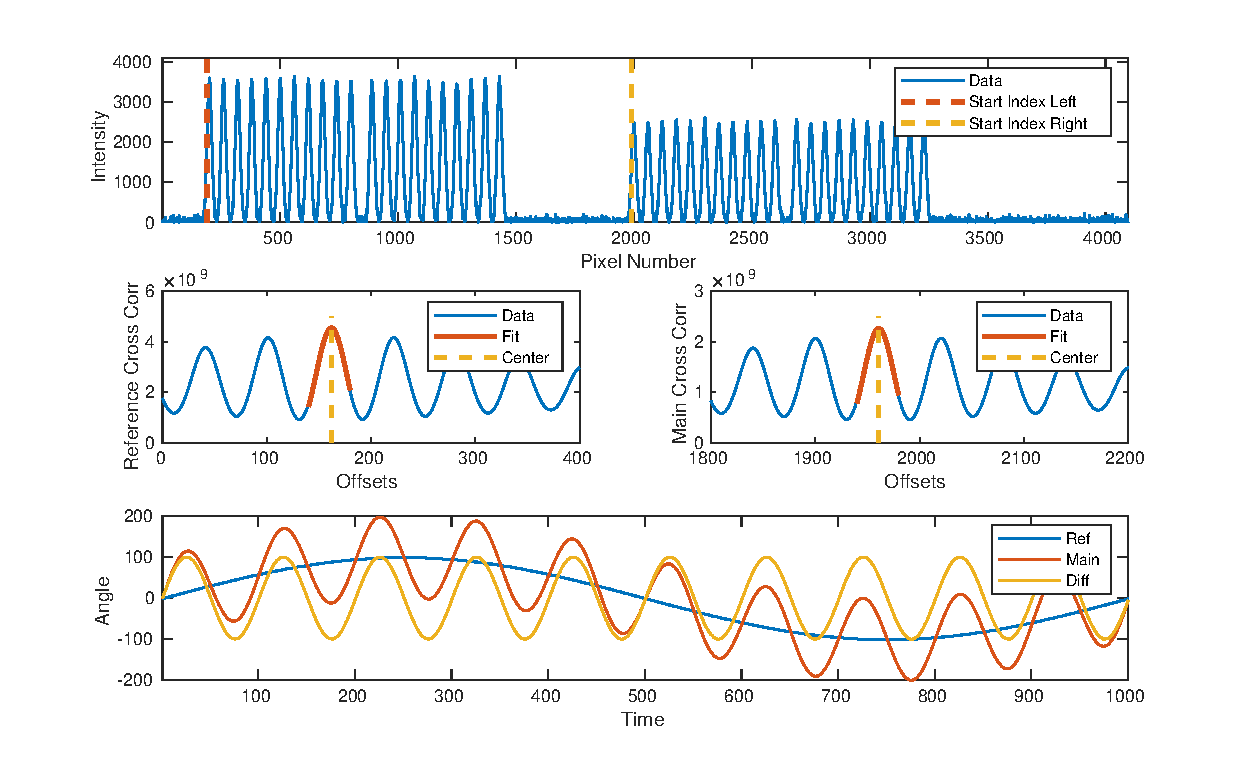
\includegraphics[width=\textwidth]{BRS_ImgAnalysis.pdf}
\caption[Simulation of the BRS image analysis algorithm]{Simulation of the BRS image-analysis algorithm. The top pane shows a simulated frame of the fringes as seen by the CCD, the middle panes show the cross-correlation and fit from the two patterns, and the bottom shows the output of the algorithm for each pattern and the difference of the two. For this simulation the main pattern was modulated at both 1 mHz and 10 mHz while the reference was at 1 mHz.}
\label{ImgAnalysis}
\end{center}
\end{figure}

To extract the distance between the patterns, the image goes through a series of steps to convert from a vector of pixel intensities to a single angular output. When the software begins, the first frame is saved. All future frames are split into two, with one part representing the reference mirror and the other the main mirror. A cross-correlation is then taken between each part and its matching section of the first frame. This gives a curve with a maximum located at the pixel number corresponding to the separation between the pattern in the current frame and the first frame, which can be seen in Figure \ref{ImgAnalysis}. The points of this curve nearest to the maximum are then fit to a Gaussian which gives the location of the peak with sub-pixel resolution. This is done for each pattern separately after which the difference between the reference pattern location and the main pattern location is taken. The difference is then proportional to the change in angle between reference mirror and main mirror following Equation \ref{ACEq}.

Compared to previous image analysis algorithms \cite{MSA}, this algorithm is computationally efficient while also being less susceptible to variations in the pattern image due to dust particulate, incorrect focusing, or beam clipping. A sensitivity of $\sim$0.3 nrad$/\sqrt{\text{Hz}}$ at 0.1 Hz was achieved with this autocollimator design and image analysis algorithm.

\subsection{Controls}

\quad As the BRSs are installed in active lab spaces, anthropogenic activity and environmental disturbances apply torques to the beam-balance through mechanical and gravitational coupling. These torques can then cause the motion at the resonant frequency to rise to undesirable amplitudes. As the beam motion increases so does the noise and the effects of non-linearities of the readout. In addition, some disturbances can cause the amplitude to exceed the dynamic range of the autocollimator readout system.

The alleviate this issue, we installed capacitor plates underneath each end of the beam-balance to act as actuators. Neglecting edge effects, the force between the two parallel capacitor plates is: 
\begin{equation}
F=\frac{\epsilon A V^2}{2d^2} \label{cap}
\end{equation}
where $\epsilon$ is the permittivity of the volume between the plates, $A$ is the area of the plate, $V$ is the voltage applied to the plates, and $d$ is the distance between the plates. The plates under the beam are connected to a digital-to-analog converter while the beam is electrically grounded so that a controlled actuation torque can be applied to the beam. 

The feedback signal sent to the capacitors was the angular velocity of the beam, band-passed between 2 mHz and 20 mHz to include only motion at frequencies near the resonance. The feedback is applied with low gain to only increase the loss of the system as compared to strong feedback where all of the motion is absorbed into the controls. This arrangement is implemented with two gain levels, a ``low amplitude'' level, which is always on and yields a $Q$ of 10-15, and a ``high amplitude'' level, which is triggered if the amplitude rises above a threshold that is set based on the properties of the given device and gives a $Q$ of 5-10.

\subsection{Noise Performance}\label{BRSNoise}

In addition to the 0.3 nrad/$\sqrt{\text{Hz}}$ frequency-independent noise of the autocollimator readout, the BRSs have a collection of mechanical noise sources, especially temperature variations and thermal motion of the flexures.

Although the exact physical mechanism is unknown, it has been observed that variations in the exterior temperature cause shifts in the instrument's equilibrium position. Furthermore, temperature gradients across the instrument emanating from unbalanced heat sources and air currents have been seen to cause time-varying noise. To alleviate this issue, the instrument's vacuum chamber and optics are wrapped in multiple alternating layers of packing foam and aluminum foil. The entire apparatus is placed inside a large double walled insulation box to further decrease any temperature variation. These improvements decrease these effects yet temperature noise is believed to limit the performance below 20 mHz.

\begin{figure}
\begin{center}
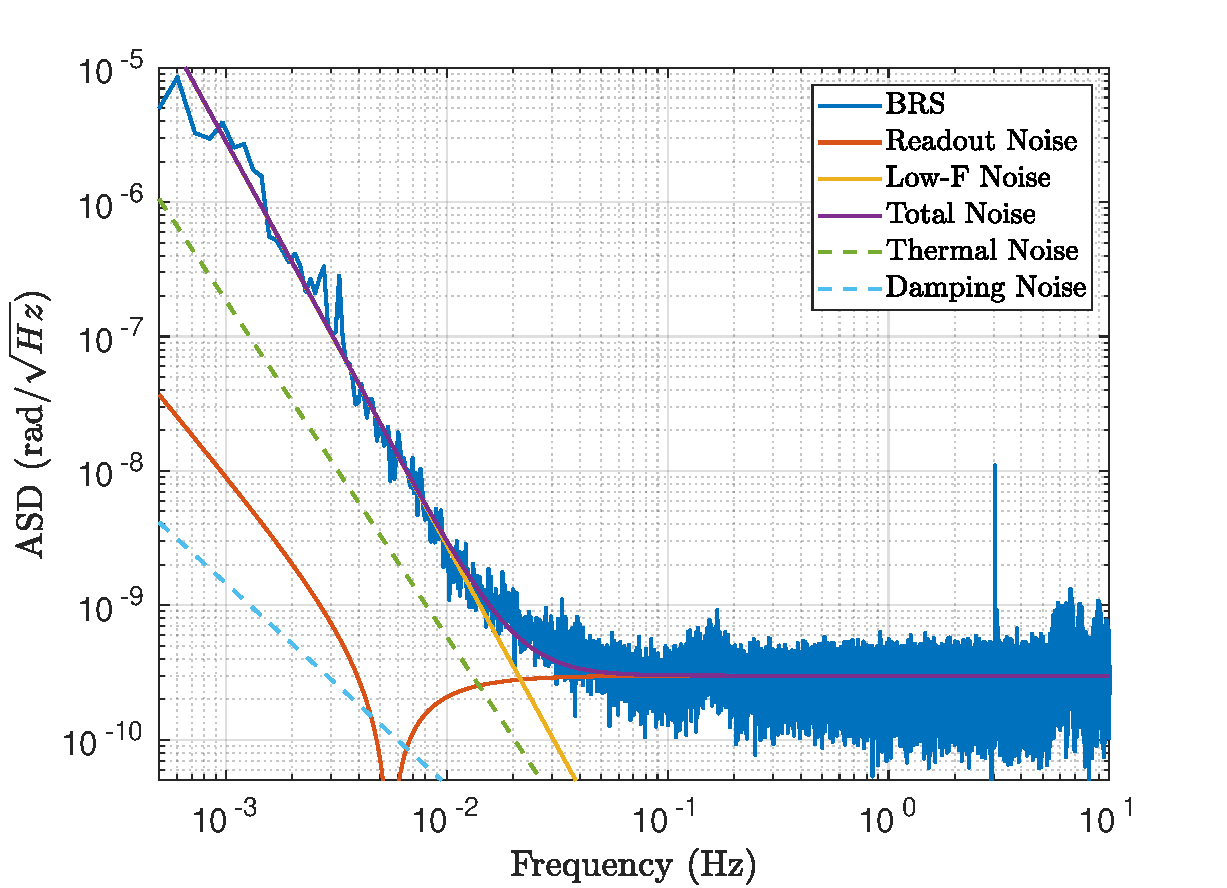
\includegraphics[width=0.85\textwidth]{BRSNoiseModel.pdf}
\caption[Noise budge for the Beam Rotation Sensors]{Noise budget for the Beam Rotation Sensors where the blue curve shows the performance at a quiet time, in red is a model of the readout noise, yellow shows an estimate of the low-frequency noise, purple shows the sum of these, and cyan and green show upper limits of the thermal and damping noise. The low-f noise is thought to be due to residual temperature variations.}
\label{noise}
\end{center}
\end{figure}

More fundamental is the noise due to thermal excitations of the flexure. At non-zero temperature, a portion of the thermal energy of the flexures excites mechanical motion. This causes a fundamental stochastic noise floor that follows \cite{thermal}:

\begin{equation}
\tilde\theta_T(\omega)=\sqrt{\frac{4 k_B T \omega_0^2}{I \omega Q\big((\omega^2-\omega_0^2)^2+\omega_0^4/Q^2\big)}}
\end{equation}

To limit the influence on the performance of the device, the resonant frequency of the spring-mass system is pushed to the lowest feasible frequency. This is the fundamental noise of the instrument, independent of readout and environmental effects.

 One further noise source comes from voltage noise on the capacitive actuators. The force follows Equation \ref{cap}. Assuming a voltage noise on the capacitors of 0.1 V/$\sqrt{\text{Hz}}$, larger than expected with the installed electronics, the corresponding torque noise is $4.3 \times 10^{-13}$ N/$\sqrt{\text{Hz}}$. This then leads to an angle noise that is $\sim$100 times below the measured noise.

 The noise budget for the LHO End-X BRS is shown in Figure \ref{noise}. It shows that the device is readout dominated above $\sim$20 mHz and below is dominated by unknown noise thought to be sourced by temperature variations. The peaks at 150 mHz, 3 Hz, and 6 Hz arise from the rotational microseism, torsion mode of the beam-balance, and motion due to nearby instrumentation, respectively.

\section{Results}\label{results}
\subsection{Hanford Installation} \label{BRS_Hanford}

\begin{figure}[!h]
\begin{center}
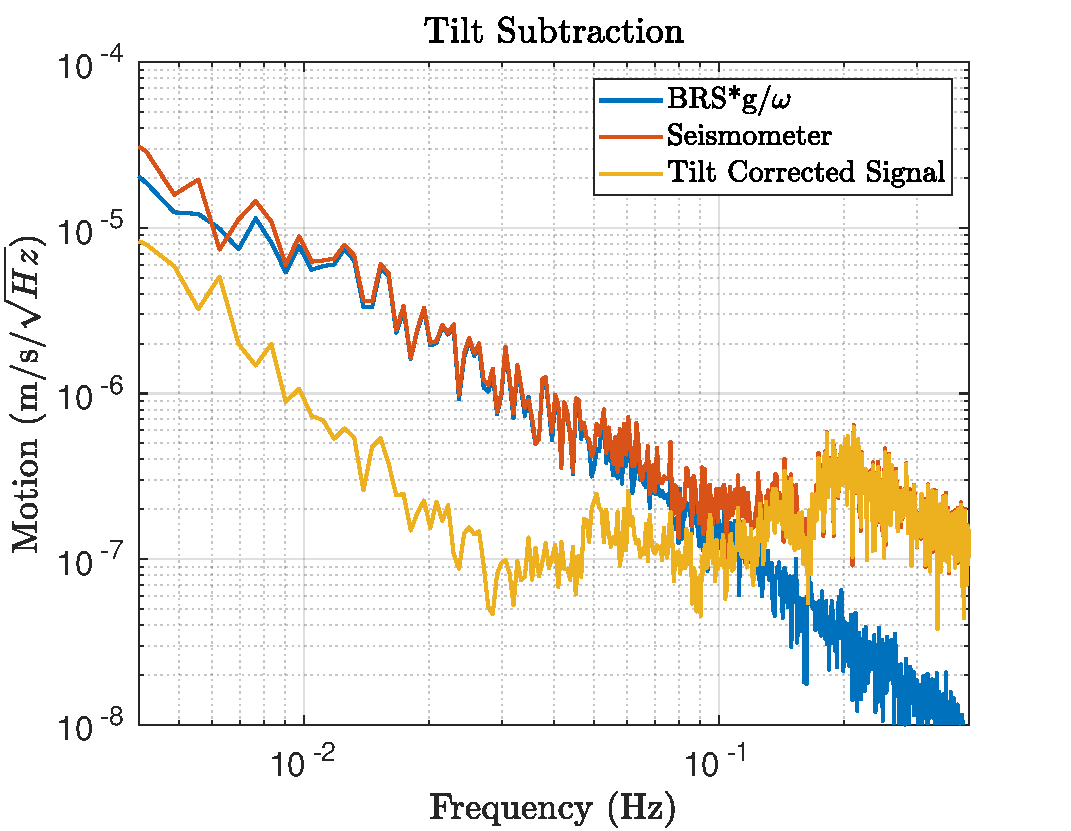
\includegraphics[width=0.85\textwidth]{TiltCorrSpec.pdf}
\caption[Representative amplitude spectral density showing the tilt subtraction during windy conditions]{Representative amplitude spectral density showing the tilt subtraction during $\sim$11 m/s winds achieved at End-X of LHO where blue is the BRS signal multiplied by $g/\omega$, read is the raw seismometer signal, and yellow is the tilt corrected signal. Similar perform has been achieved by all of the deployed BRSs.}
\label{sub}
\end{center}
\end{figure}

\quad A BRS was installed at each of the end stations of the LIGO Hanford Observatory (LHO) between the first (O1) and second (O2) observing runs. Each device was used to correct the translation along the respective arm of the interferometer.\footnote{Motion orthogonal to the interferometer arms couples only indirectly through pathways such as defects of the test masses and mechanical cross couplings. Thus this coupling is significantly suppressed compared to motion along the arms.} Although one would expect that the corner station seismometers would also need to be corrected, a location was found within the corner station building which exhibited low tilt.\footnote{This location had low tilt because of it's distance from the walls of the building.} As such no BRS was necessary to achieve low tilt contamination.


The tilt subtraction performance achieved with these devices can be seen in Figure \ref{sub} where it is evident that the system achieves tilt subtraction from around 6 mHz to 50 mHz. Above 50 mHz the seismometer signal is dominated by the oceanic microseism and the tilt contribution is negligible. Below 6 mHz, the BRS signal becomes overwhelmed by instrumental noise. This performance can also be seen in Figure \ref{subTime} which shows a example time series of the tilt subtraction where suppression of a handful of transients, likely due to wind gusts, can be seen.

\begin{figure}[!h]
\begin{center}
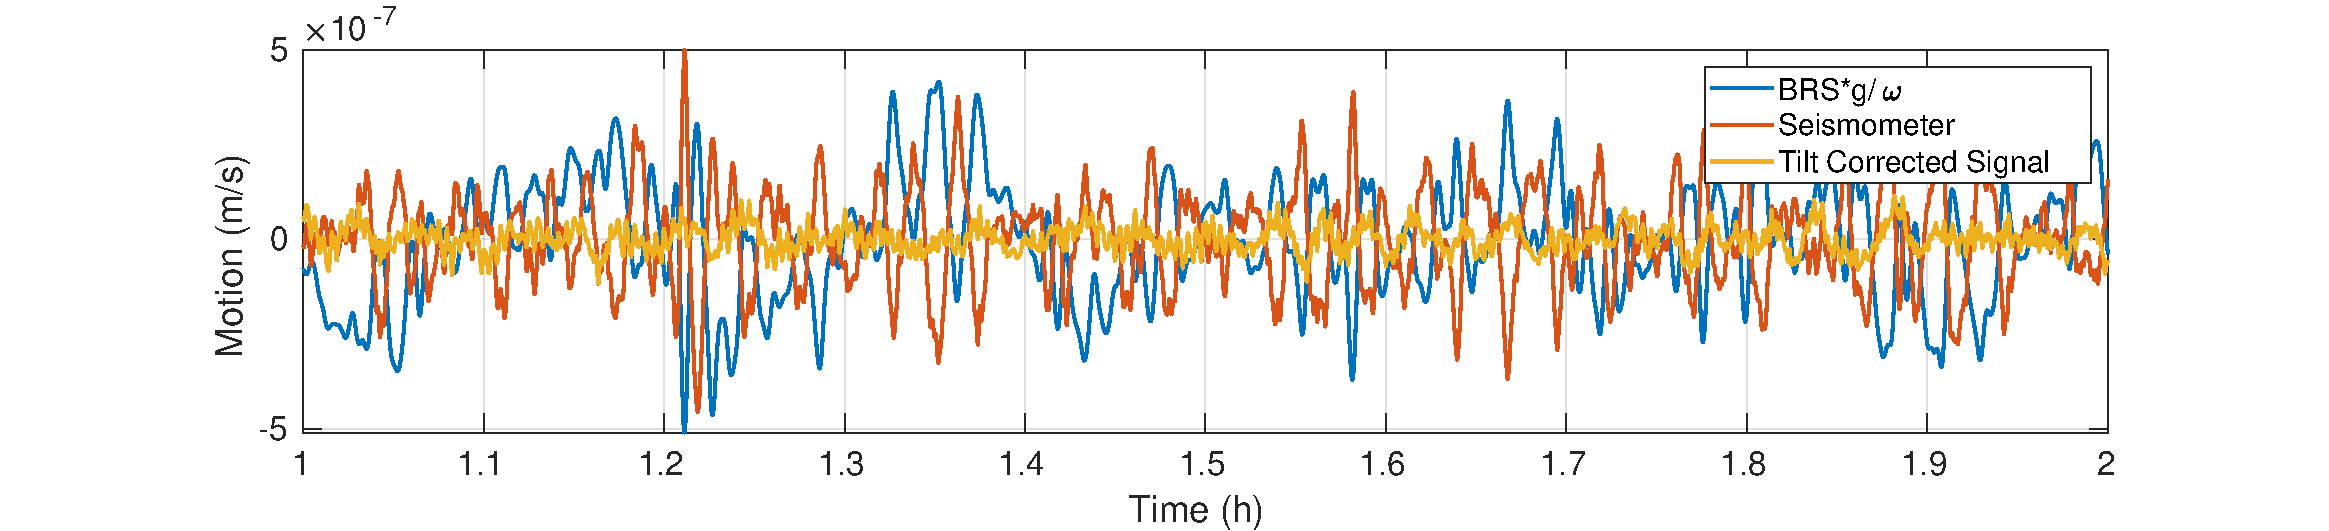
\includegraphics[width=\textwidth]{TiltCorrTime.pdf}
\caption[Time series showing tilt subtraction ]{Time series showing the tilt subtraction at End-X of LHO where blue is the BRS signal multiplied by $g/\omega$, read is the raw seismometer signal, and yellow is the tilt corrected signal. All channels are band-passed from 10-100 mHz. As can be seen, the tilt subtraction removes a collection of transients, likely due to the gusts of wind.}
\label{subTime}
\end{center}
\end{figure}

This tilt-subtracted channel, rather than the raw seismometer, was then used as the ground signal for the isolation system's sensor correction, described in Section \ref{SensCor}. The primary effect on the interferometer of using this channel is a decrease in the differential motion between pairs of platforms which form the arms of the interfrometer. Figure \ref{armMotion} shows that the differential motion was decreased by a factor of $\sim$3-4 between 20-100 mHz. This increases the ability to lock the interferometer by decreasing the demand on the downstream control systems.

\begin{figure}[!h]
\begin{center}
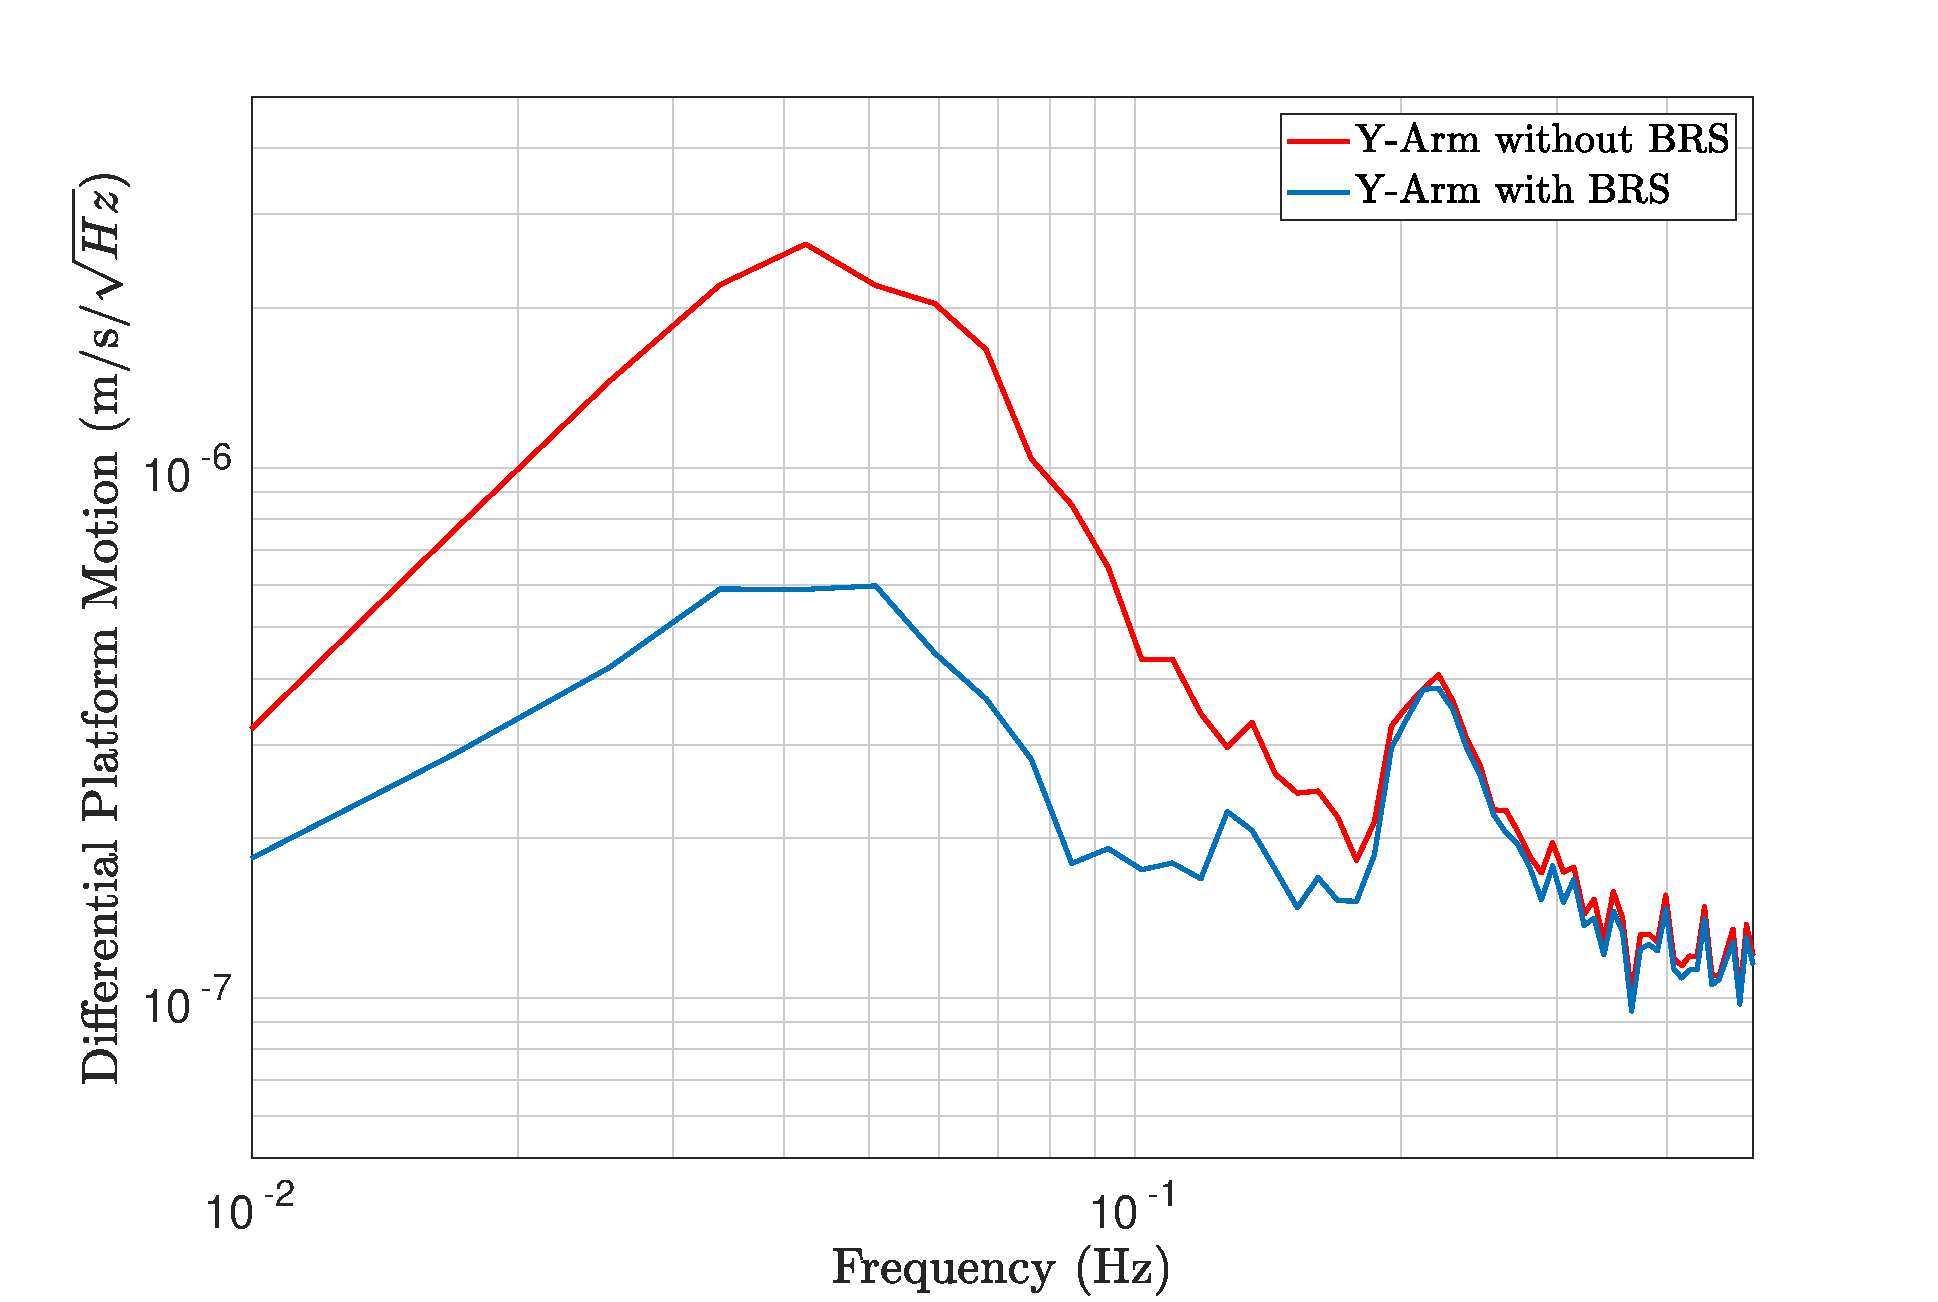
\includegraphics[width=0.85\textwidth]{BRSArmMotion.pdf}
\caption[Differential platform motion ]{Differential platform motion as measure by the capacitive position sensors (CPS) for the Y-Arm of LHO with and without the BRSs installed. Below $\sim$30 mHz, the CPS reading is driven to zero by the control system.}
\label{armMotion}
\end{center}
\end{figure}

\subsection{Livingston Installation}

\quad After the success of the Hanford BRS installation, four devices were installed at the LIGO Livingston Observatory (LLO) between the second and third (O3) observing runs. Due to differences in the size and shape of the corner station building at LLO, a low tilt location was not found. Therefore BRSs were installed near the input test masses along with one at each end station. Each device corrected the seismometer readings along the corresponding interferometer arm. 

All four devices achieved comparable tilt-subtraction as the Hanford installation and were implemented in a similar fashion. 

\subsection{Ground Tilt Model}


As mentioned in Section \ref{tiltCon}, the primary driver of ground tilts at the observatories is wind acting on the building's walls which deforms the concrete floor in a non-trivial manner. Thus modeling the ground tilt spectrum for a given wind speed from first principals is intractable. However, with the collection of observations made by the BRSs installed at the sites, an empirical model can be readily constructed.

To achieve this, hour long spectra of the BRS output at the End-X of LHO during O3a were sorted into a collection of bins depending on the average wind speed measured during that hour. Each bin was then averaged to yield a representative spectrum for each wind speed. This was then fit to an empirically determined model, Equation \ref{TiltModelEq}, containing two terms: the first constituting the broad behavior of the spectrum and a second which enhances the high frequency motion at high wind speeds. The parameters of this were then fit vs wind speed to yield a tilt spectrum vs wind speed model. 

\begin{figure}[!h]
\begin{center}
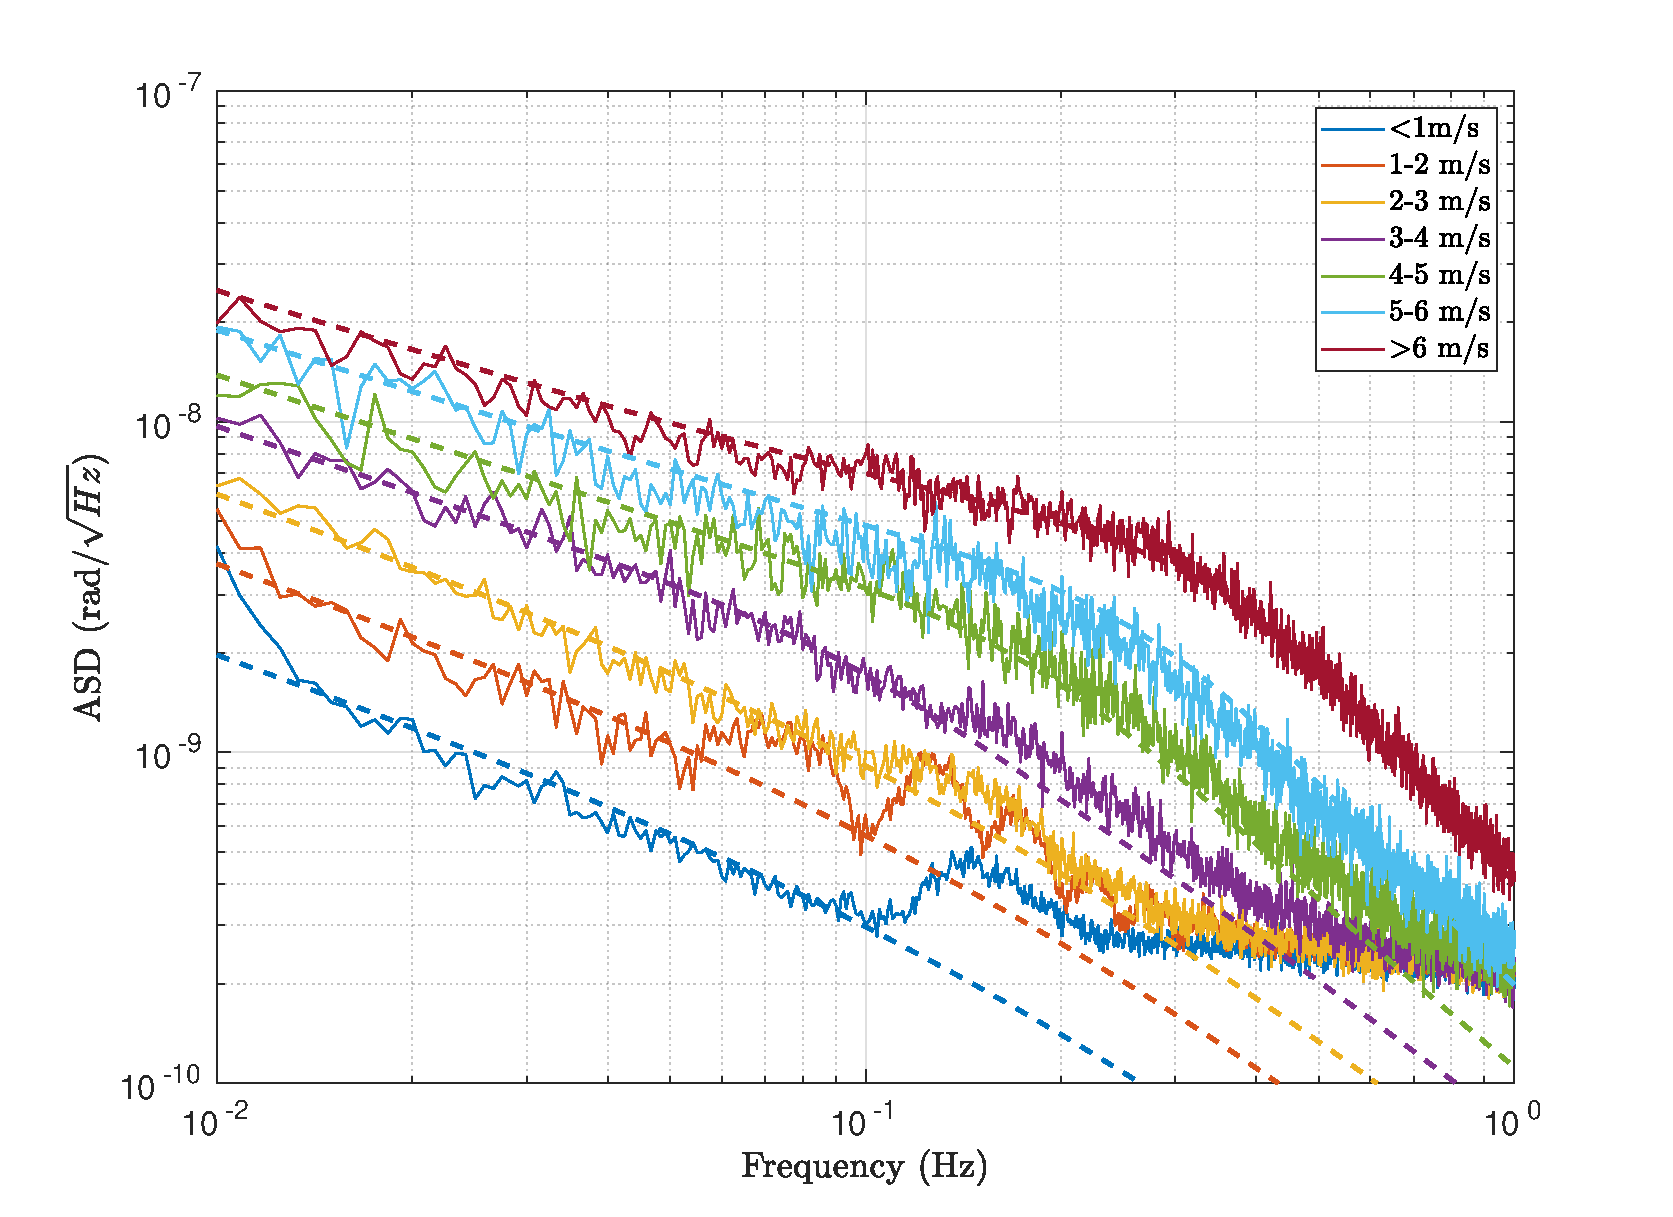
\includegraphics[width=\textwidth]{TiltModel.pdf}
\caption[Observed and modeled tilt vs wind speed]{Observed and modeled tilt vs wind speed for LHO End-X. The solid lines are the measured ground tilt while the dashed are the model. At low wind speeds, the BRS noise and the microseism become dominate at high frequencies.}
\label{tiltModel}
\end{center}
\end{figure}

\begin{align}
\tilde{\theta}&=\frac{x_1}{(f/1\text{ Hz})^{2/3}(1+f/f_1)} +\frac{x_2}{1+(f/f_2)^3}\label{TiltModelEq}\\
\nonumber \\ 
f_1&=0.2\ \text{Hz}\nonumber \\
f_2&=(0.1\ (s/\text{1 m/s}) -0.25)\ \text{Hz}\ \text{if }s>2.5\text{ m/s}\text{ else }f_2=0\nonumber \\
x_1&=(1.4\times10^{-11}\ (s/\text{1 m/s})^2+5.7\times10^{-11}\ (s/\text{1 m/s})+6.4\times10^{-11})\ \text{rad}/\sqrt{\text{Hz}}\nonumber \\
x_2&=(1.8\times10^{-10}\ (s/\text{1 m/s})^2-7.6\times10^{-10}\ (s/\text{1 m/s})+1.2\times10^{-9})\ \text{rad}/\sqrt{\text{Hz}}\nonumber
\end{align}

Here $s$ is the wind speed, $f$ is the frequency, and $\tilde{\theta}$ is the tilt spectral density. Comparison of this model to data is shown in Figure \ref{tiltModel} which shows good agreement at most wind speeds. Below 1 m/s, the tilt due to the microseismic motion and the sensor noise become dominate above 100 mHz. Between 1-2 m/s, the data was corrupted by local anthropologic activity above $\sim$50 mHz. This model can be utilized to calculate the theoretical performance of the seismic isolation, as is done in Section \ref{IsoScheme}.

\subsection{Duty Cycle Improvements}

The figure of merit which most readily displays the improvements in duty cycle due to inclusion of the BRSs is the empirical probability of the interferometer being locked at a given wind speed over the three observing runs. This is shown in Figures \ref{LHO_events} and \ref{LLO_events} for LHO and LLO, respectively. It should be noted that BRSs were implemented at Hanford for both O2 and O3a while Livingston was only for O3a.

\begin{figure}[!h]
\begin{center}
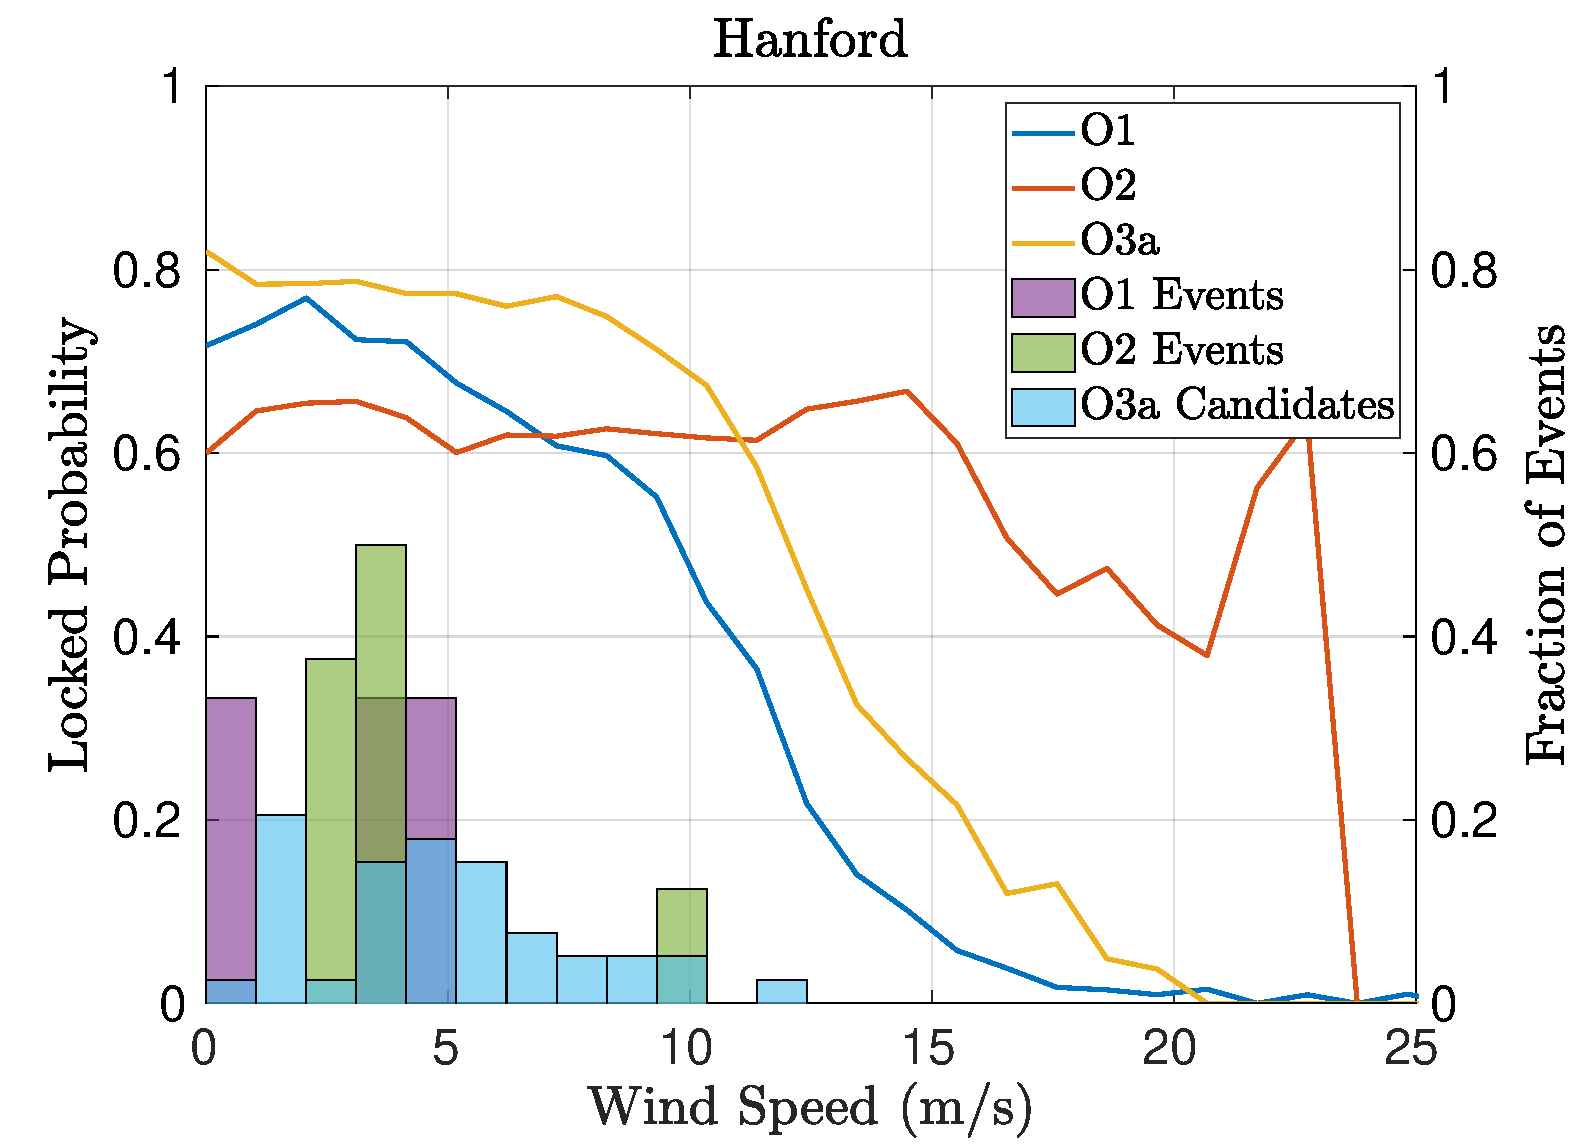
\includegraphics[width=\textwidth]{LHO_WindVsLockEvents.pdf}
\caption[Duty cycle improvements for the LIGO Hanford Observatory]{Duty cycle improvements for the LIGO Hanford Observatory along with distribution of observed events vs. wind speed. }
\label{LHO_events}
\end{center}
\end{figure}

For Hanford, the benefit of the tilt subtraction scheme can clearly be seen between O1 and O2 curves. During O1 the locked probability fell monotonically with wind speed, while for O2 the probability stayed relatively constant up to 15 m/s above which it fell steadily. For O3a, Hanford saw a clear decrease in performance at high wind speeds yet still out performed the O1 scheme. This loss of performance is likely due to the Y-arm beam being displaced away from the center of the test masses to avoid point absorbers on the Input-Y test mass.This is known to increase coupling between the angular motion of the test mass and the length measured by the interferometer. This then increases the drive needed to keep the interferometer locked and thus increases the susceptibility of the system to increased seismic motion. 

If one allows for a fudge factor to be applied to the O2 duty cycle in order to match the low wind speed performance of O1 and O3a, then this duty cycle equates to an observing time increase of 13.1 days per year between O1 and O2 and a decrease of 2.9 days/year between O2 and O3a.

Also shown in Figure \ref{LHO_events} is the fraction of the GW events or candidates detected during O1, O2, and O3a at a given wind speed. This shows that a collection of GW events have been observed whose detection probability is directly increased due to the increase duty cycle at higher wind speeds. Namely, GW170104 was measured at $\sim$11 m/s which had an increase in duty cycle of $\sim$20 \% between O1 and O2. Additionally, a number of O3a candidates have been detected above $\sim$5 m/s at which the probability of being locked is increased by $\sim$20 \%.

\begin{figure}[!h]
\begin{center}
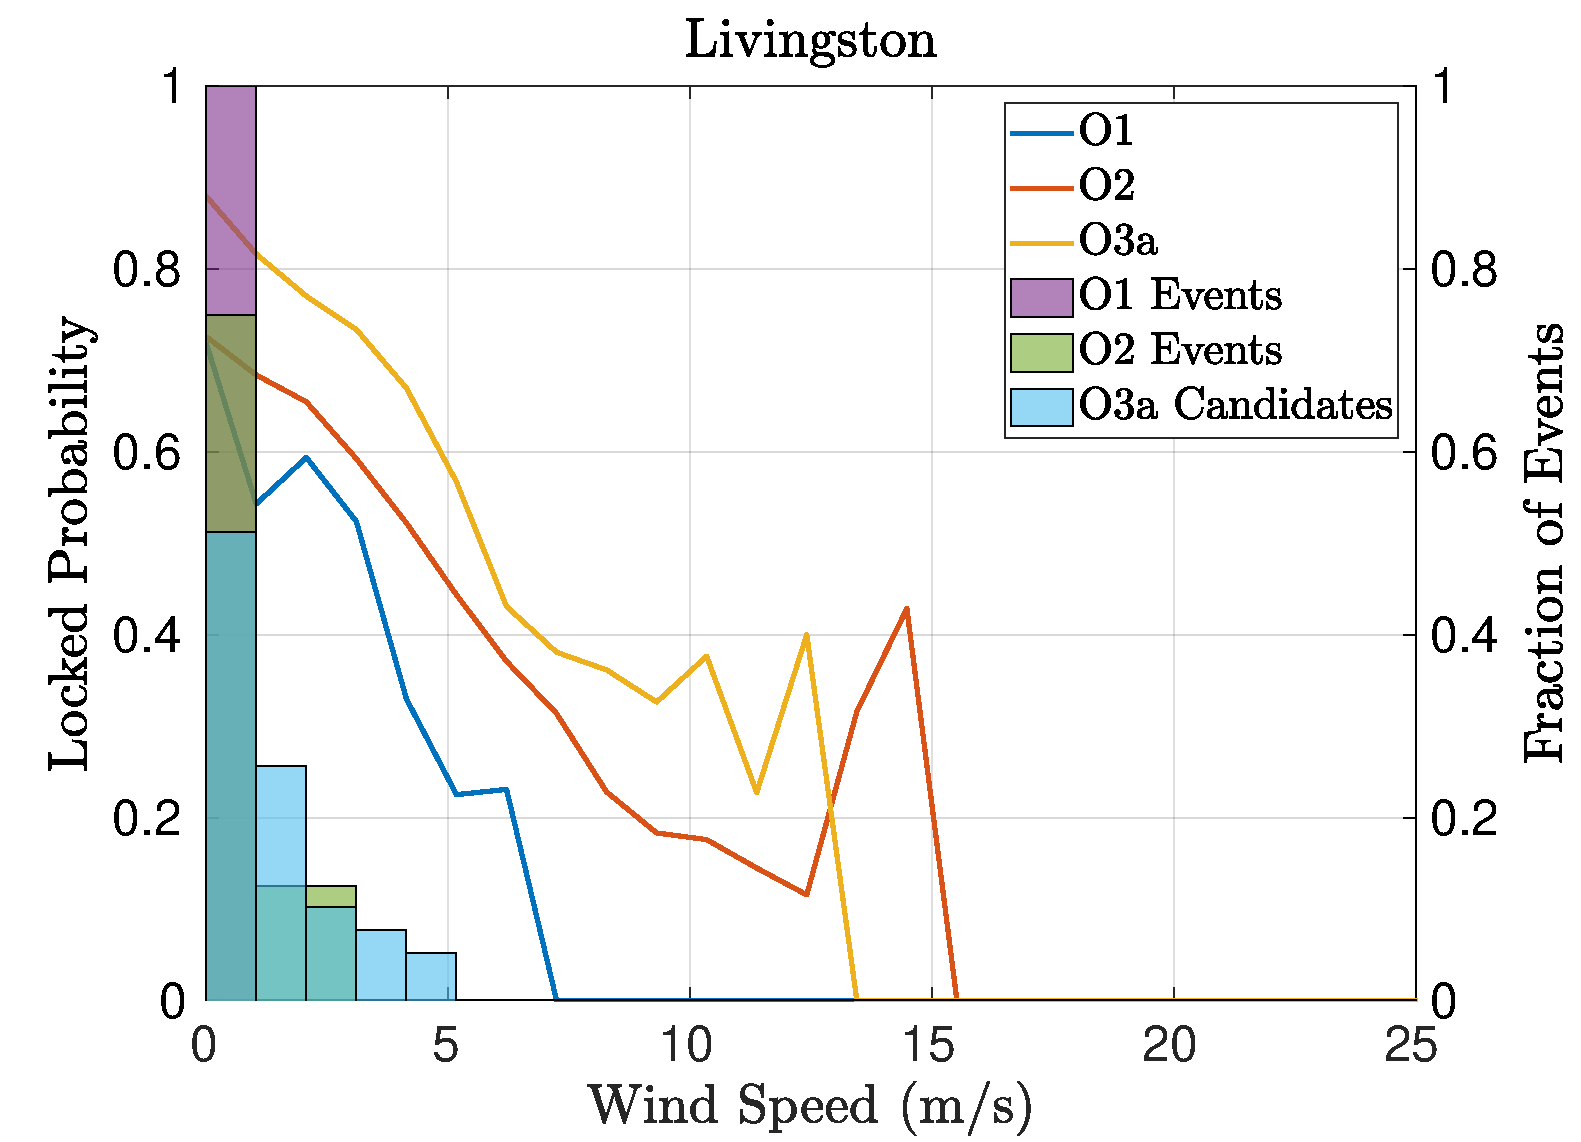
\includegraphics[width=\textwidth]{LLO_WindVsLockEvents.pdf}
\caption[Duty cycle improvements for the LIGO Livingston Observatory]{Duty cycle improvements for the LIGO Livingston Observatory along with distribution of observed events vs. wind speed.}
\label{LLO_events}
\end{center}
\end{figure}

At Livingston, the improvements at increased wind speeds is less dramatic as can be seen in Figure \ref{LLO_events}. Although between O1 and O2 tilt subtraction was not implemented, a increase in duty cycle was achieved by implementing a single seismometer for sensor correction on all of the corner station platforms. This decreased the differential mode motion at higher wind speeds and thus made the interferometer lock more robust. An additional increase in performance can be seen between O2 and O3a due to the deployment of tilt subtraction. However, the probability of being locked still dropped monotonically with wind speed, similar to the O1 performance of Hanford.

Despite this, there is a collection of O3a candidates detected between 3-6 m/s which are more probable with the increased robustness against wind speed. Additionally, this performance equates to an observing time increase of 13.9 days per year between O1 and O2 and 6.9 days/year between O2 and O3a.

An additional metric that quantifies the improved robustness of the interferometer is the expectation value of wind speed during gravitational wave events which is shown in Figure \ref{WindExp}. In the limit that the detection likelihood is independent of wind speed, one would expect that the expectation value of the wind speed during events would match that of the entire run. As can be seen in Figure \ref{WindExp}, with the installation of the BRSs each site approaches this limit. 

\begin{figure}[!h]
\begin{center}
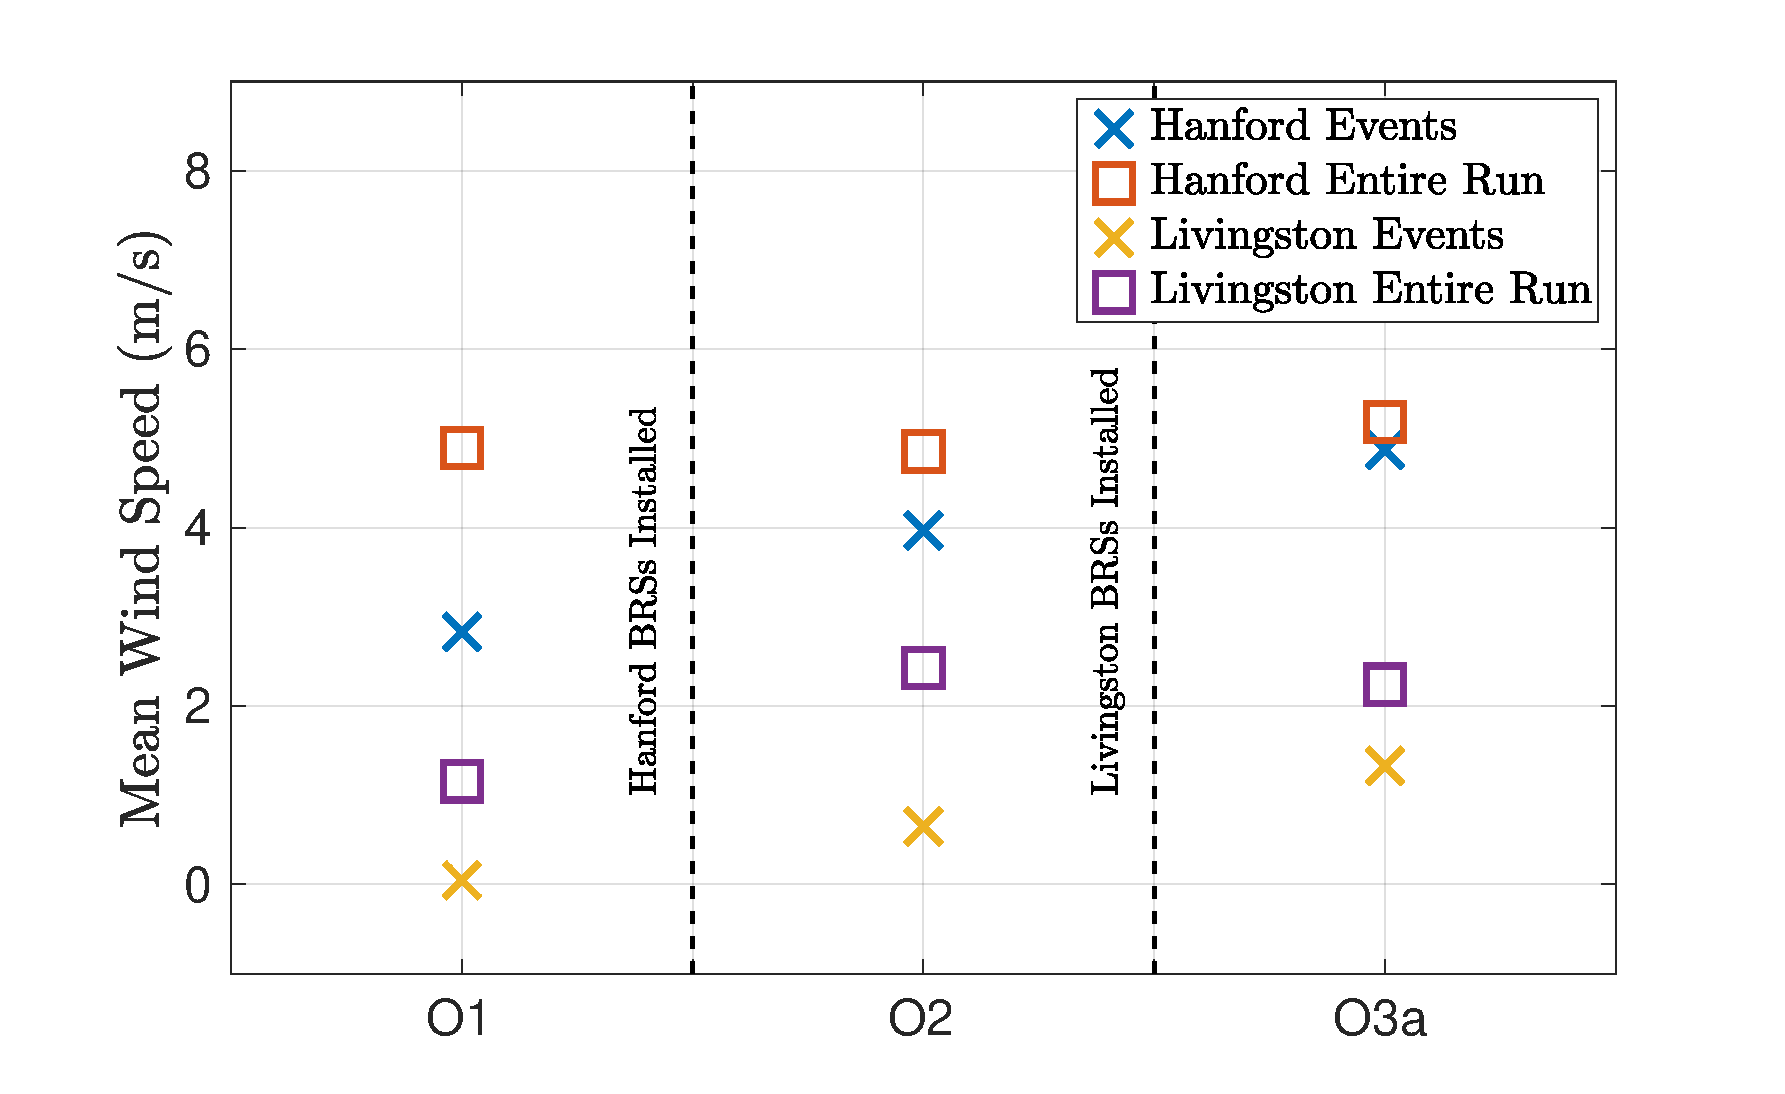
\includegraphics[width=\textwidth]{WindExpect.pdf}
\caption[Expectation value of wind speed during GW events]{Expectation value of wind speed during gravitational wave events and for the entire observing runs.}
\label{WindExp}
\end{center}
\end{figure}


\chapter{30-cm Scale On-Board Rotation Sensors}\label{cBRS_chap}
\section{Angular Controls}\label{ASC}
\begin{figure}[!h]
\begin{center}
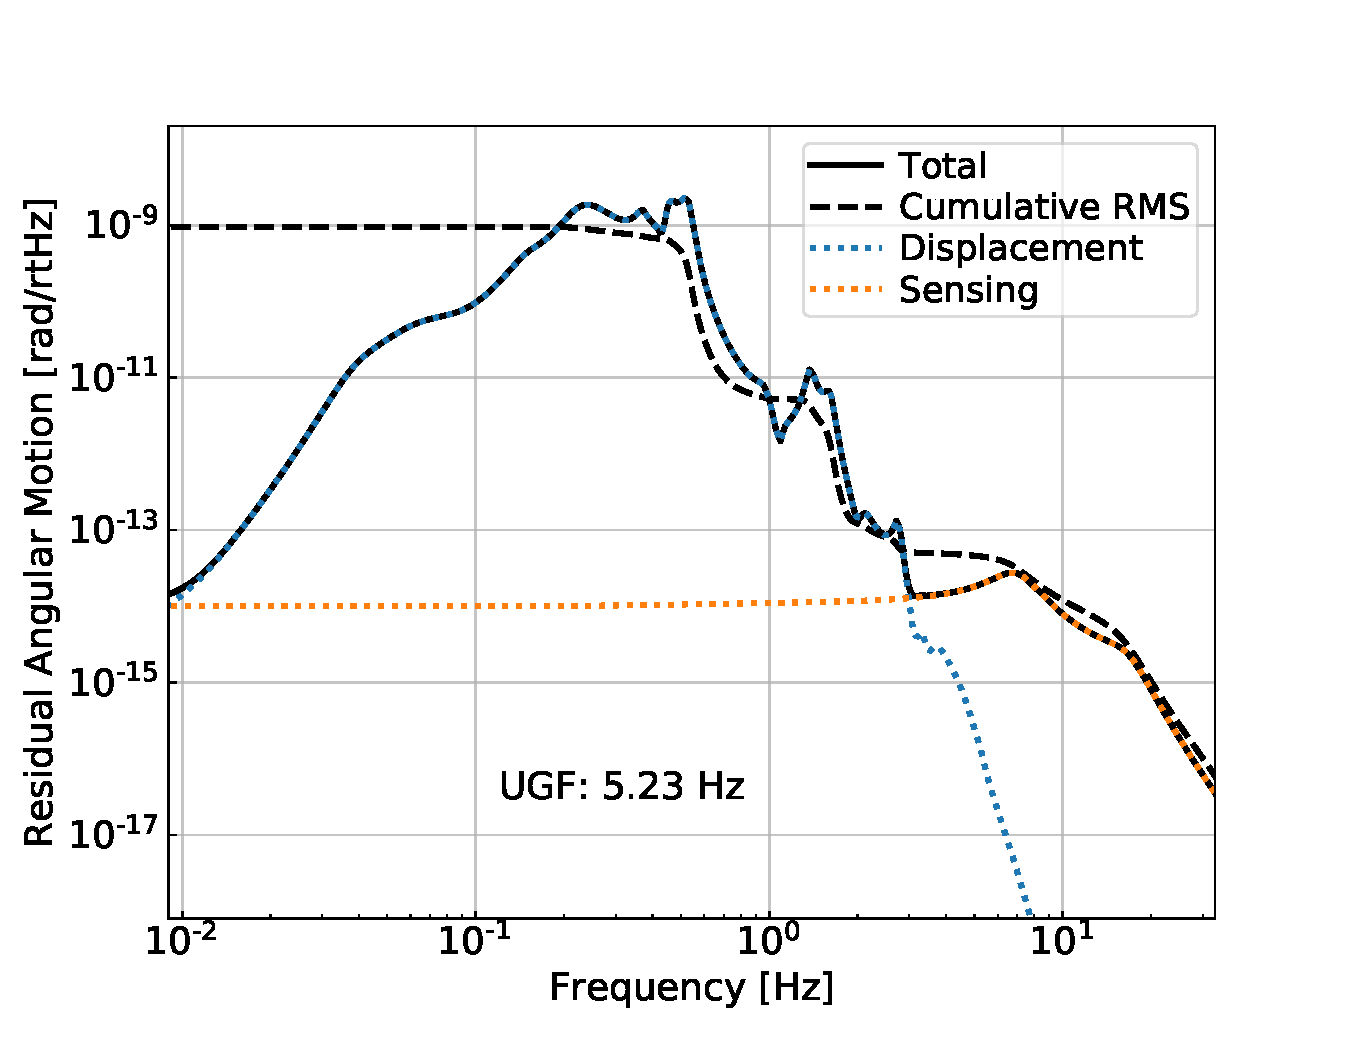
\includegraphics[width=\textwidth]{cBRS_ASC_Without.pdf}
\caption[Model of the performance of the current angular sensing and control system]{A model of the performance of the current angular sensing and control system. This model optimizes the unity gain frequency of the ASC loop to maximize performance above $\sim$10 Hz while maintaining the low frequency rms at 1 nrad/$\sqrt{\text{Hz}}$.}
\label{ascWithout}
\end{center}
\end{figure}
To operate the LIGO interferometers in their optimal configuration, the relative angular motion of the test masses must be under 1 nrad rms \cite{ASC}. Although the seismic isolation system significantly attenuates the input motion to the optics, additional controls are needed to meet this requirement. The angular sensing and control system (ASC) consists of a number of optical sensors which are fed back to actuators on the quadruple pendulum. 

With the current seismic isolation system, at $\sim$0.2 Hz the rotational performance is limited by the sensor noise in the seismometer pair which forms the isolation platform's angular sensors \cite{windproofing}. This then increases the residual translational motion due to tilt contamination, described in Section \ref{tiltCon}. To eliminate this residual, high-gain feedback loops are required on the downstream ASC system, which themselves are limited by their respective sensor noise above $\sim$3 Hz. This left over noise then leaks into the gravitational wave band between 10 - 55 Hz due to the inability to sharply roll off the sensor noise without interfering with the control at lower frequencies. A model of the current ASC system is shown in Figure 3.1.

\begin{figure}[!h]
\begin{center}
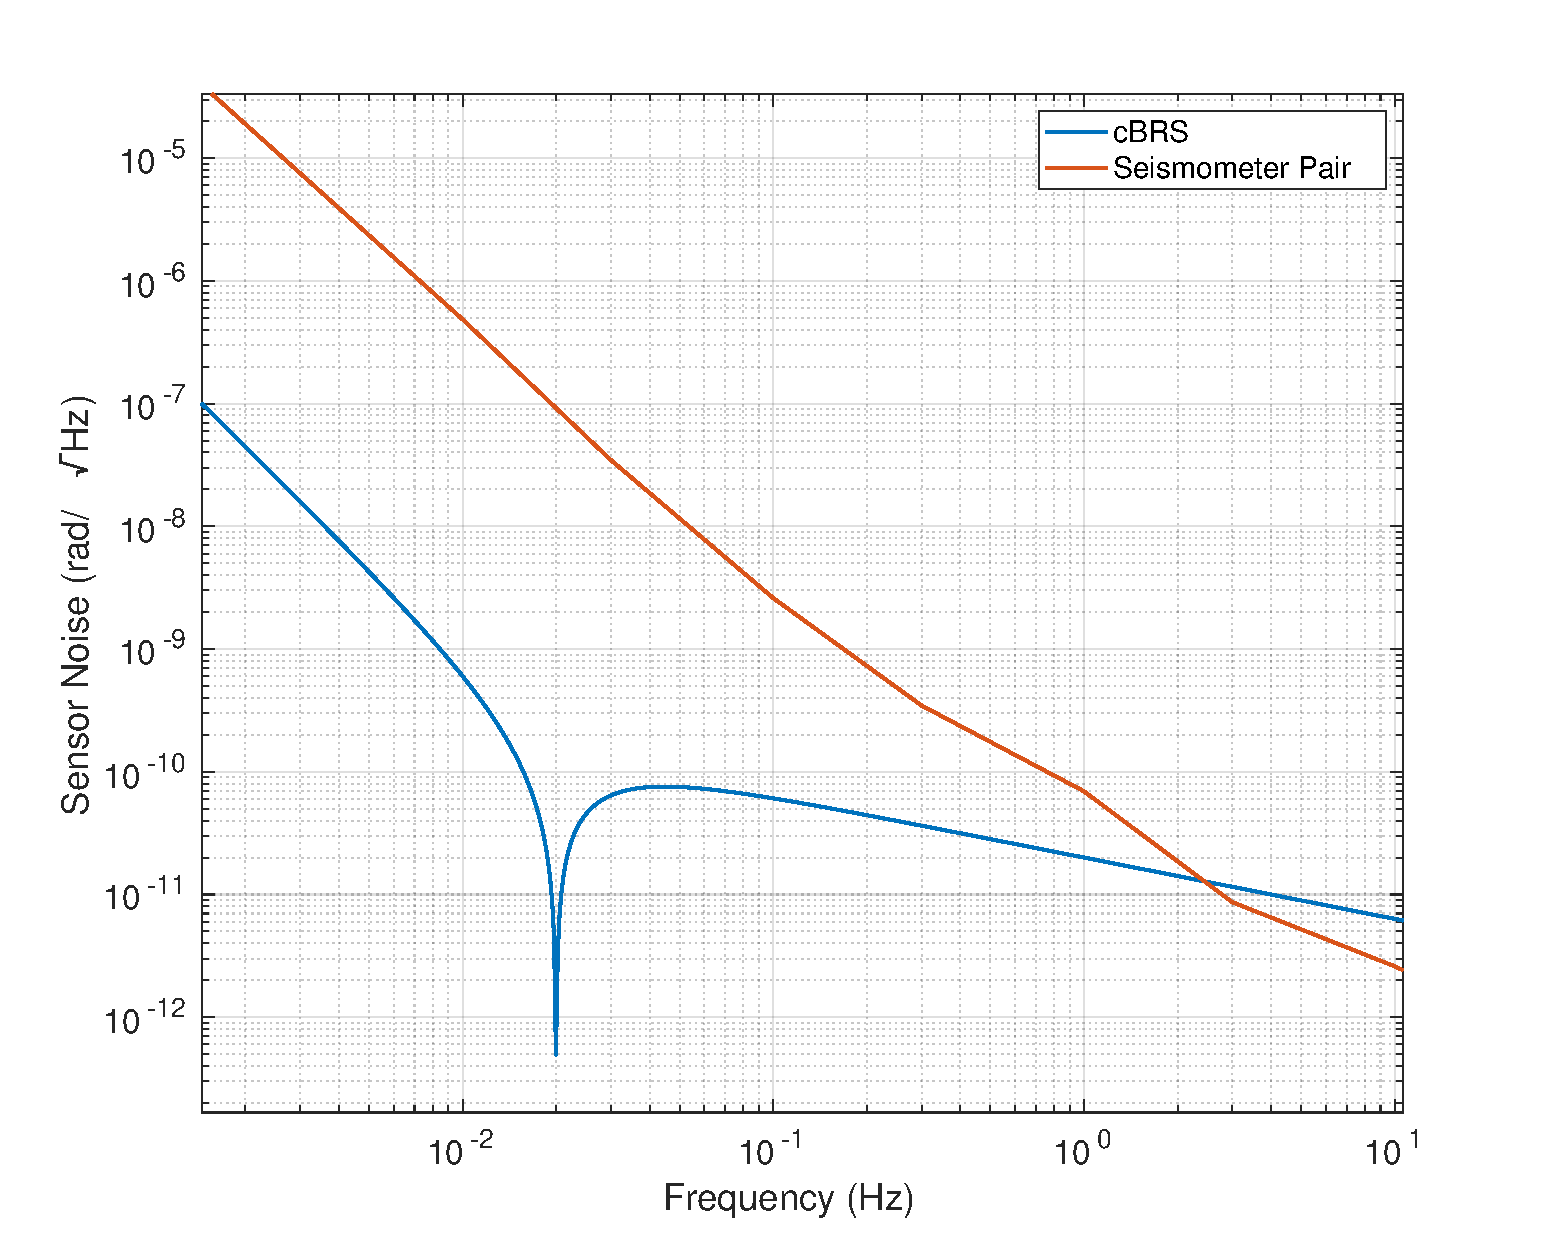
\includegraphics[width=0.85\textwidth]{sensorNoise.pdf}
\caption[Theoretical noise curves for the cBRS and seismometer pair]{Theoretical noise curves for the cBRS, blue, and seismometer pair located 1-m apart.}
\label{sensNoise}
\end{center}
\end{figure}


The compact Beam Rotation Sensor (cBRS), described in the following, was designed to be an alternative angular sensor for the seismic isolation system with $\sim$100-1000 times lower noise than the current sensors. Design sensitivity of the cBRS and the current seismometer pair are shown in Figure \ref{sensNoise}. With this decreased noise, the seismic isolation control loops can be tuned to significantly increase the performance of both the translational isolation, through decreased tilt contamination described in Section \ref{tiltCon}, and, directly, the rotational isolation. Details of this follow in Section \ref{IsoScheme}. This decreased residual rotation would then allow the angular control loops to be retuned, specifically decreasing the unity gain frequency (UGF), to decrease the sensor noise leakage in the gravitational wave band.

Additional benefits are also expected to accompany the improved seismic isolation. This include decreased effects of scattered light and increased robustness against environmental effects. Beforehand modeling these effects are intractable but will be studied in detail for future installations.


\section{Compact Beam Rotation Sensor} \label{cBRSSec}
\subsection{Mechanical System}

Similar to the BRS described in Chapter \ref{BRS_chap}, the compact Beam Rotation Sensor (cBRS), shown in Figure \ref{cBRS1}-\ref{cBRS2}, consists of a 30-cm long cross hung from 10-15 $\mu$m thick beryllium-copper flexures and has an identical operating principle as the BRS. Above the resonant frequency the beam acts as an inertial reference whose angle is measured with respect to the support. Thus Equations \ref{theta_A}-\ref{theta_s} govern its mechanics. The cross shape of the balance decreases the sensitivity of the device to gradients in the local gravitational field while allowing for increased moment of inertia compared to a similarly sized beam. 

This design yields a resonant frequency of $\sim$20 mHz which limits the use of such a device with high fidelity to frequencies about and above this. This removes the possibility of using such a device for ground tilt subtraction since the relevant ground tilts happen below 40 mHz. 

\begin{figure}[!h]
\begin{center}
\includegraphics[width=0.75\textwidth]{cBRSIso.png}
\end{center}
\caption[CAD rendering of the cBRS]{CAD rendering of the compact BRS (cBRS) showing the cross with its copper end masses which is hung from the flexures from the surrounding support structure. Additionally, the translation stages which hold the fiber interferometer readouts can be seen on either end of the support below the two horizontal end masses.}
\label{cBRS1}
\end{figure}


\begin{figure}[!h]
\begin{center}
 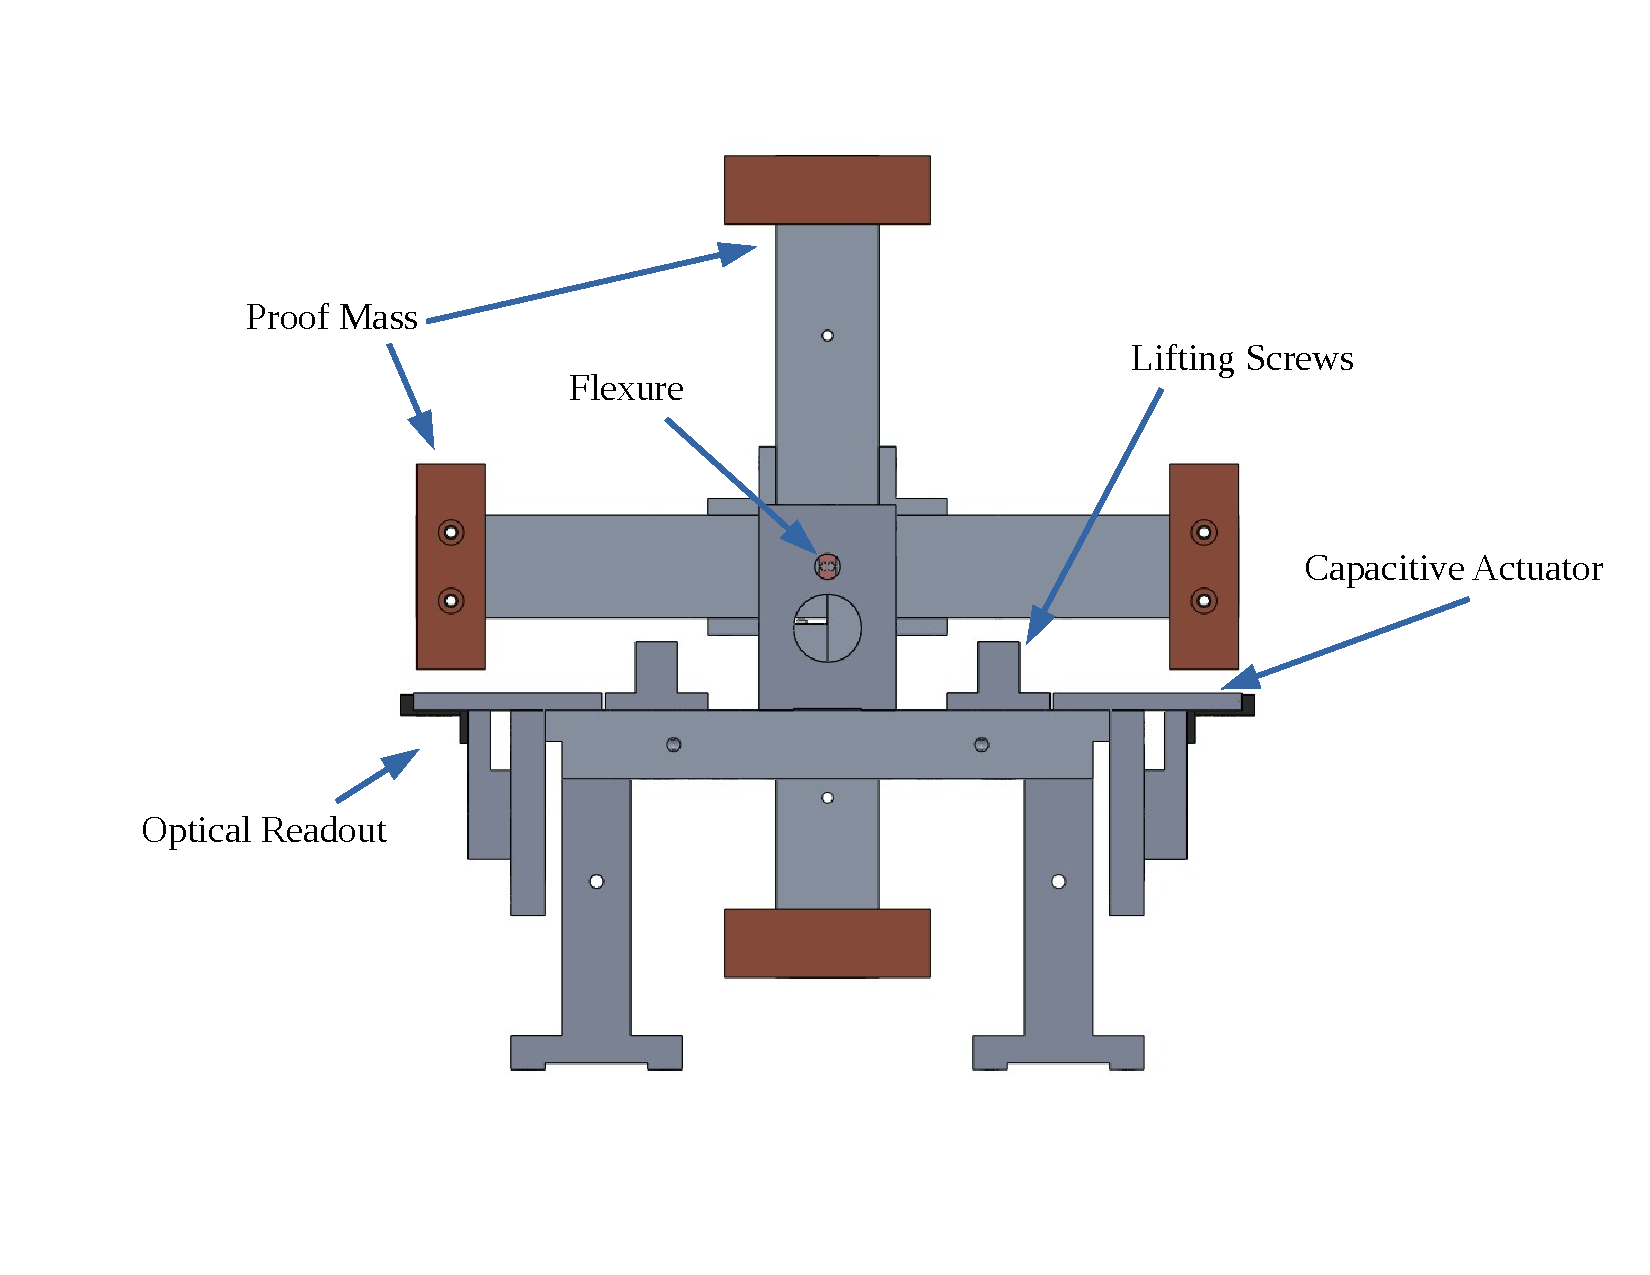
\includegraphics[width=\textwidth]{cBRSFrontLabeled.pdf}
 
\caption[Side view of the CAD rendering of the cBRS]{CAD rendering of the compact BRS (cBRS) showing the cross with its copper end masses which is hung from the flexures from the surrounding support structure. Additionally, the translation stages which hold the fiber interferometer readouts can be seen on either end of the support below the two horizontal end masses.}
\label{cBRS2}
\end{center}
\end{figure}

\subsection{Kinematic Mount}

To allow for ease of installation, the proof mass is suspended via a kinematic mount, shown in Figure \ref{kmount}. The mount consists of three titanium spheres which are attached to the proof mass's horizontal beam and three pairs of titanium cylinders attached to a seat. This seat is then suspended by flexures, described in Section \ref{flex}. The spheres and cylinders are epoxied in place to form an equilateral triangle.

This design allows for the delicate procedure of clamping the flexures to be done with only the seat. After which the proof mass is lowered on to the seat where the matching sets of spheres and cylinders repeatably constrains its position relative to the flexures.

\begin{figure}[!h]
\begin{center}
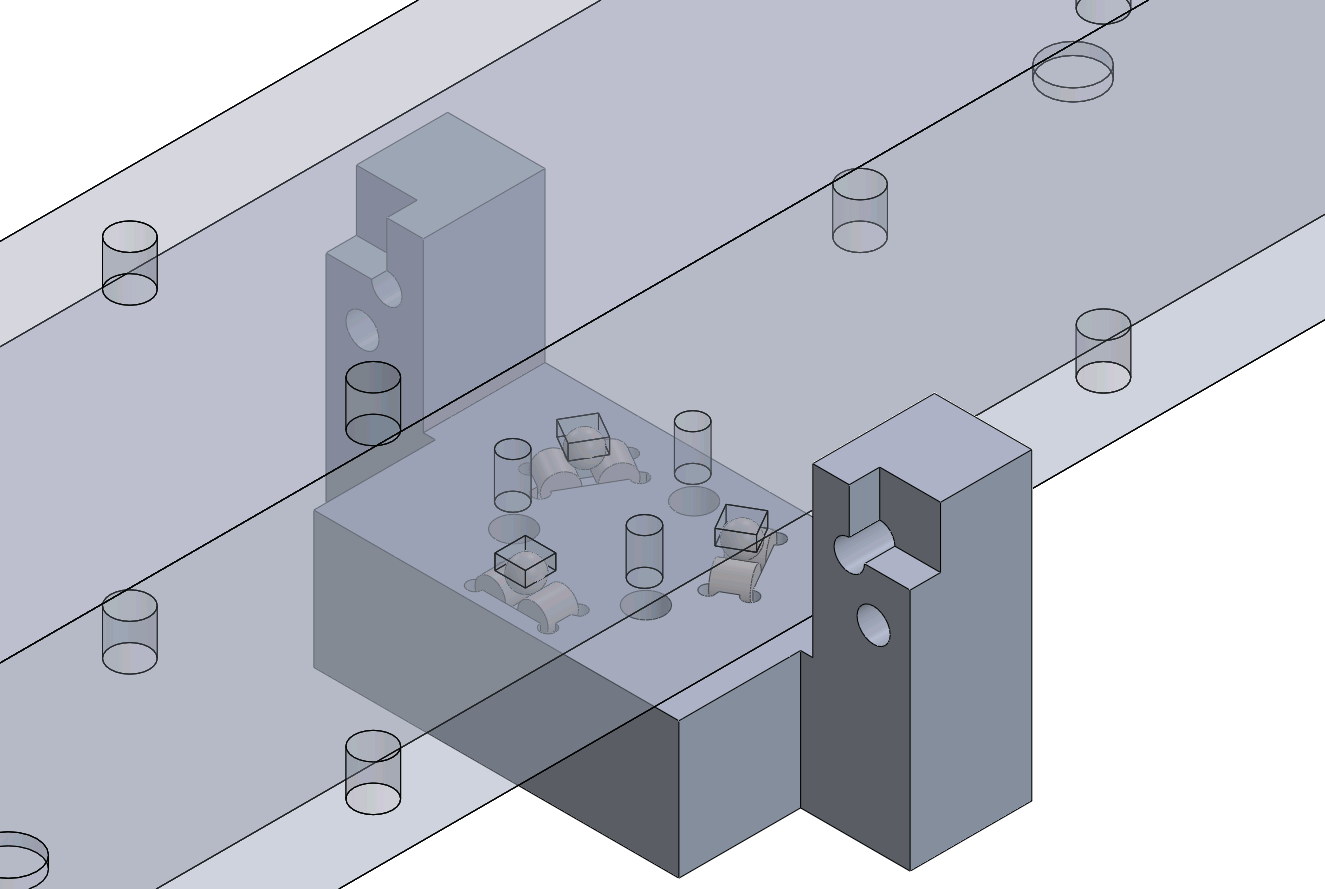
\includegraphics[width=0.75\textwidth]{cBRSKMount.png}
\end{center}
\caption[CAD rendering of the cBRS kinematic mount]{CAD rendering of the compact BRS (cBRS) showing the cross with its copper end masses which is hung from the flexures from the surrounding support structure. Additionally, the translation stages which hold the fiber interferometer readouts can be seen on either end of the support below the two horizontal end masses.}\label{kmount}
\end{figure}

\subsection{Interferometric Readout}
In order to maintain the small size of the entire device and to decrease readout noise, an interferometric readout was developed that consists of a Fabry-Perot cavity formed by a beamsplitter-coated optical-fiber and a full-reflecting mirror placed on the bottom of the balance's end masses, shown in Figure \ref{cBRSOpt}. The reflectance of this cavity is then monitored by employing a circulator to seperate the incoming and outgoing rays. The readout optics are schematically shown in Figure \ref{cBRSOptLay}. As the cavity length changes the reflectence undergoes an interference pattern described by:

\begin{align}
R=\frac{F \sin^2(2\pi n x/\lambda)}{1+F \sin^2(2\pi n x/\lambda)}
\end{align}

where $R$ is the reflectance, $F$ is the finesse, $x$ is the length of the cavity, $n$ is the index of refraction of the cavity, and $\lambda$ is the wavelength.

\begin{figure}[!h]
\begin{center}
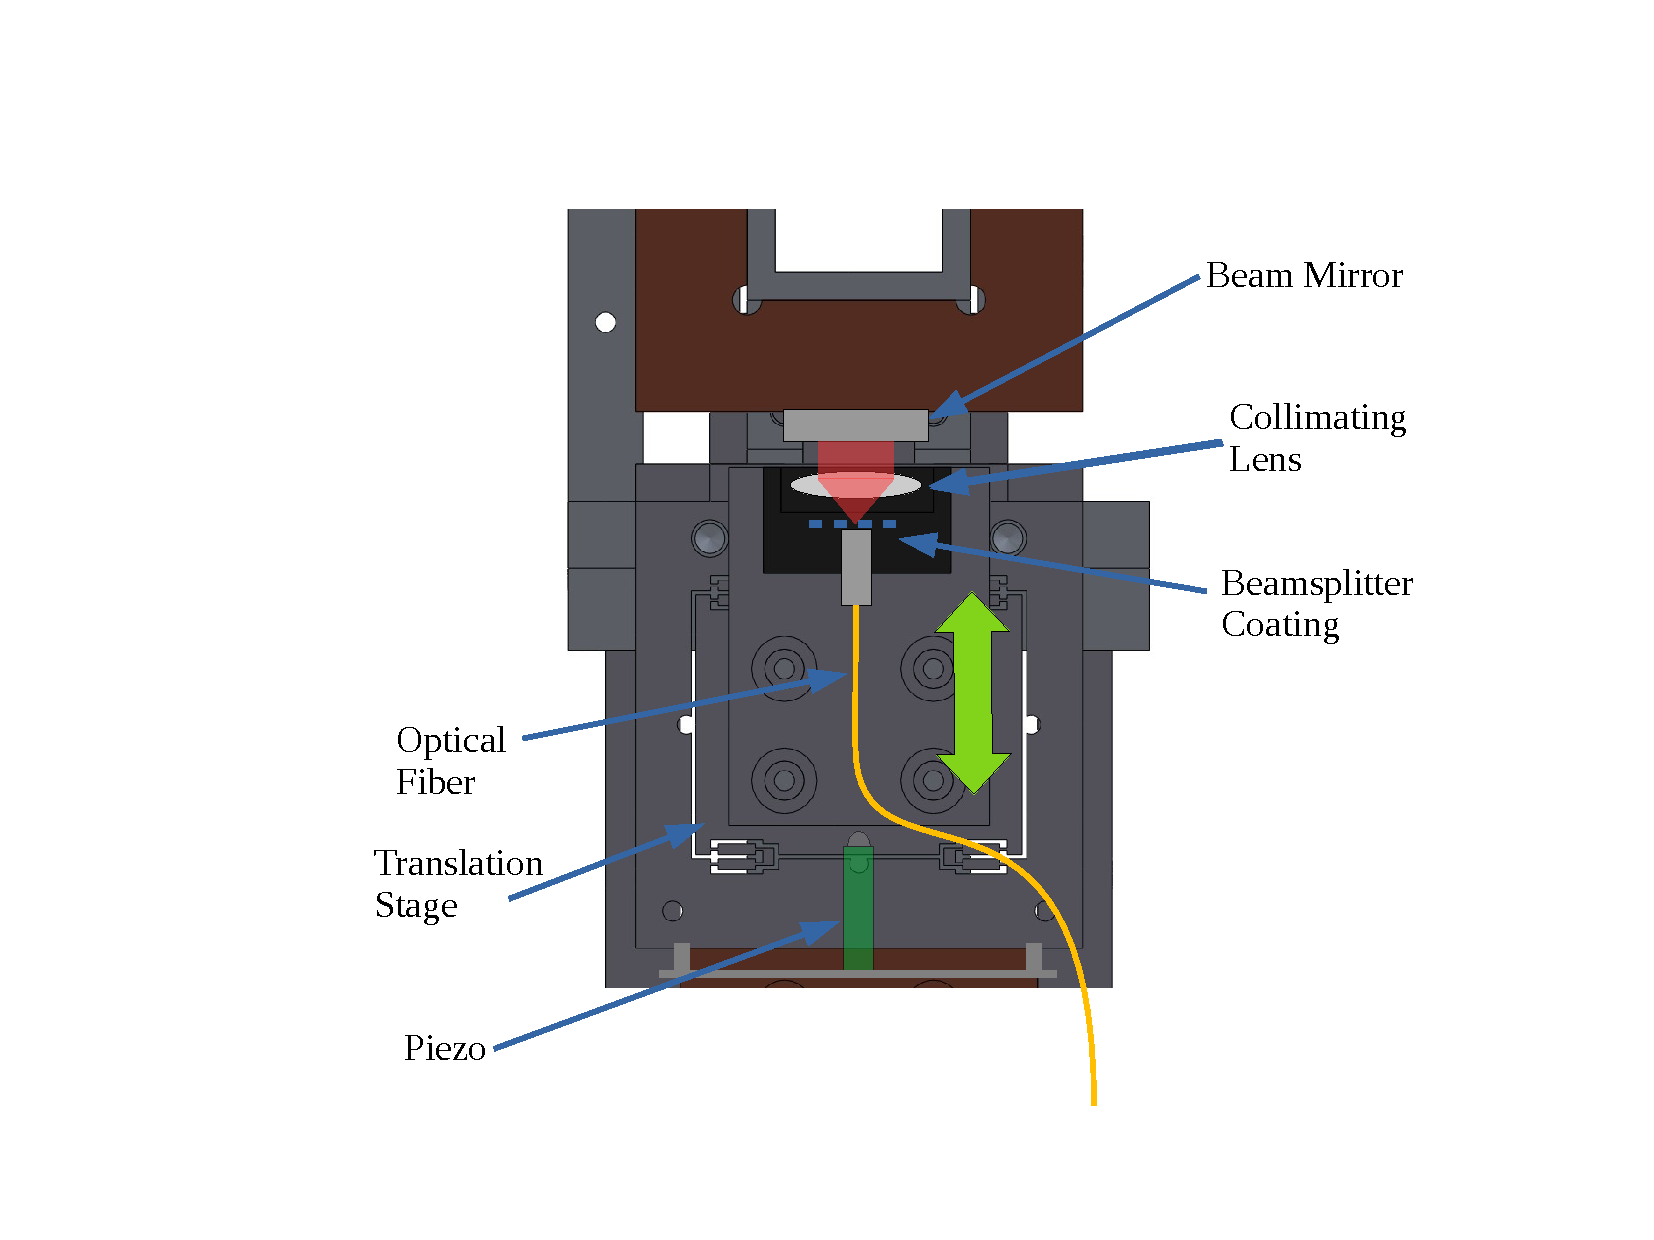
\includegraphics[width=\textwidth]{cBRSOptics.pdf}
\end{center}
\caption[Diagram of the cBRS fiber interferometer read-head]{Diagram of the cBRS fiber interferometer read-head.}
\label{cBRSOpt}
\end{figure}

\begin{figure}[!h]
\begin{center}
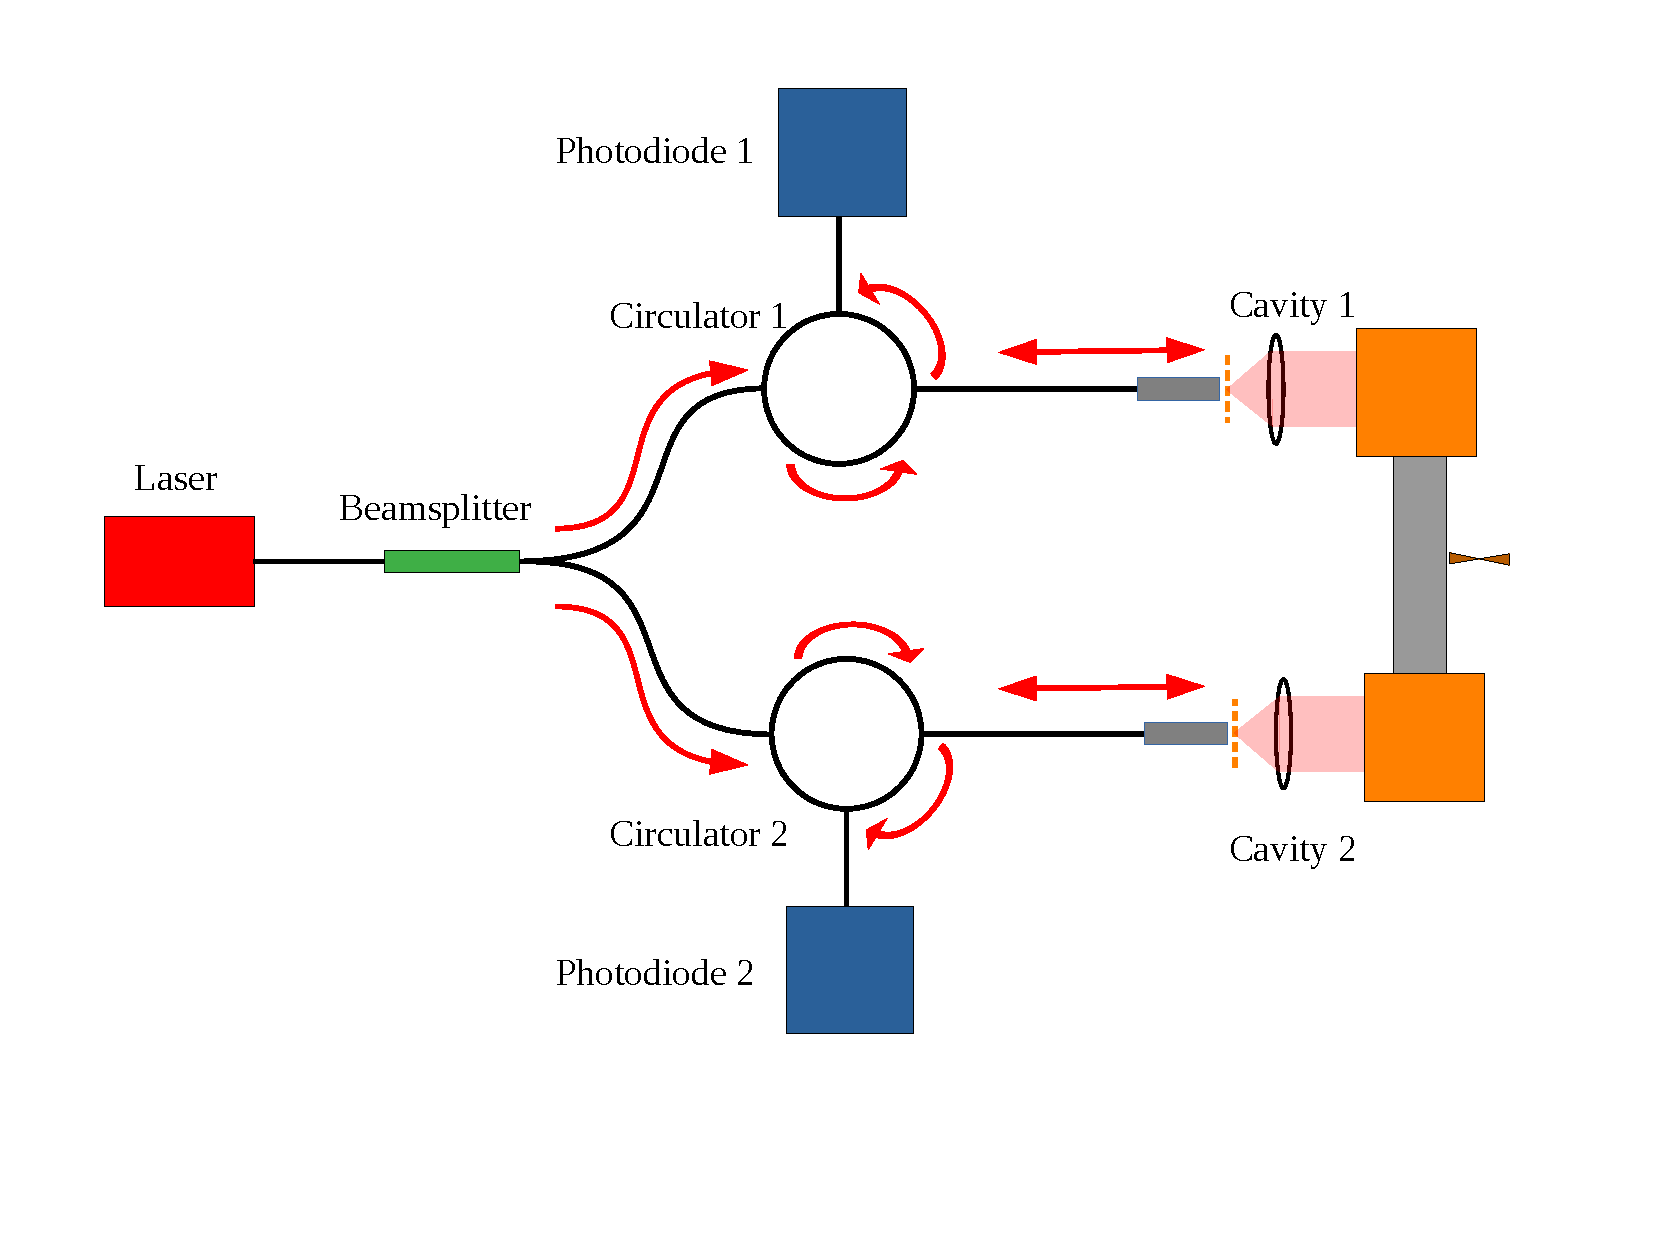
\includegraphics[width=\textwidth]{cBRS_OpticalLayout.pdf}
\end{center}
\caption[Layout of the cBRS readout optics]{Layout of the cBRS readout optics.}
\label{cBRSOptLay}
\end{figure}

To linearize this readout, the optical fiber tip and collimating lens are placed on a translation stage that is driven by a piezo stack. The intensity of the reflected light is then fed back to the piezos using a PID loop to hold the cavity length fixed. This allows the system to be seperated into two linear readouts, the interferometer output for small ranges above the UGF of the loop and the control loop output for large motions below the UGF. The output of the device is then the sum of these two channels.


Although in theory the angle of the beam can be measured with a single interferometer, two readouts are deployed, one at the end of each arm, in order to allow for suppression of common mode noise. The signal seen in each readout is described by:

\begin{align}
\theta_1&=\theta_s+x_1/L+x_1 \delta_\lambda/\lambda^2+n_c+n_1 \label{th1} \\
\theta_2&=-\theta_s+x_2/L+x_2 \delta_\lambda/\lambda^2 + n_c+n_2 \label{th2}
\end{align}

Where $\theta_{1,2}$ are the angle equivalent signal seen in readout 1 and 2, $\theta_{s}$ is the sensed angle, $x_{1,2}$ are the length of the respective cavities, $L$ is the arm length of the beam, $\delta_\lambda$ is the change in wavelength of the laser, $\lambda$ is the wavelength of the laser, $n_c$ is the sum of all unmodeled common noises, and $n_{1,2}$ are the unmodeled noises that appear in one readout and not the other.

\begin{center}
\begin{tabular}{| c | c |}
\hline
Parameter & Value\\
\hline \hline
Laser & QPhotonics QDFBLD-1300-10\\
Wavelength & 1310 nm\\
Fiber beamsplitter & Thorlabs TWQ1300HA\\
Circulator & Thorlabs CIR1310-APC\\
Fiber-tip beamsplitter & Thorlabs SMF28ER 50/50 FC/PC\\
Collimating focus & 2.75 mm\\
Photodiode & Thorlabs PDA10CS InGaAs\\
Piezo & Tokin AE0505D16F\\
Piezo Max Range & 17.4 $\mu$m at 150 V\\
Piezo Driver & PDu150 150 V\\
\hline
\end{tabular}
\label{cBRSTable}
\end{center}

As the angle of the beam appears with opposite phase in the two readout, the difference between the two, Equation \ref{diffEq}, contains the angle while suppressing common noise. Most notable of these common noise sources is frequency noise of the laser. This couples to the angle only through the mismatch in the average cavity lengths which are matched to within 1 mm. On the other hand, the sum of the two channels, Equation \ref{sumEq}, contains no contribution from the angle but is instead comprised of only noise sources and thus allows for an in-situ estimate of the sum of noises.


\begin{align}
\Delta \theta&=2\theta_s+ (x_1-x_2)\delta_\lambda/\lambda^2+n_1-n_2 \label{diffEq} \\
\Sigma \theta&=(x_1+x_2)/L+ (x_1+x_2)\delta_\lambda/\lambda^2+2n_c+n_1+n_2 \label{sumEq}
\end{align}

\subsection{Calibration}

The two readouts are calibrated independently to take into account differing piezo calibration and amplifier gains. The calibration is done by driving the piezo linearly through its entire range while the beam is locked. During this drive the interference pattern wraps through multiple fringes as the cavity length is decreased. The minima of these fringes is known to be separated by $\lambda/2$ which allows for the calibration from the voltage across the piezo to displacement. The region around the 50\% reflectance point, which is the operating point of the interferometer, is then fit to a linear function of displacement to yield a calibration from reflectance to displacement.  

\begin{figure}[!h]
\begin{center}
 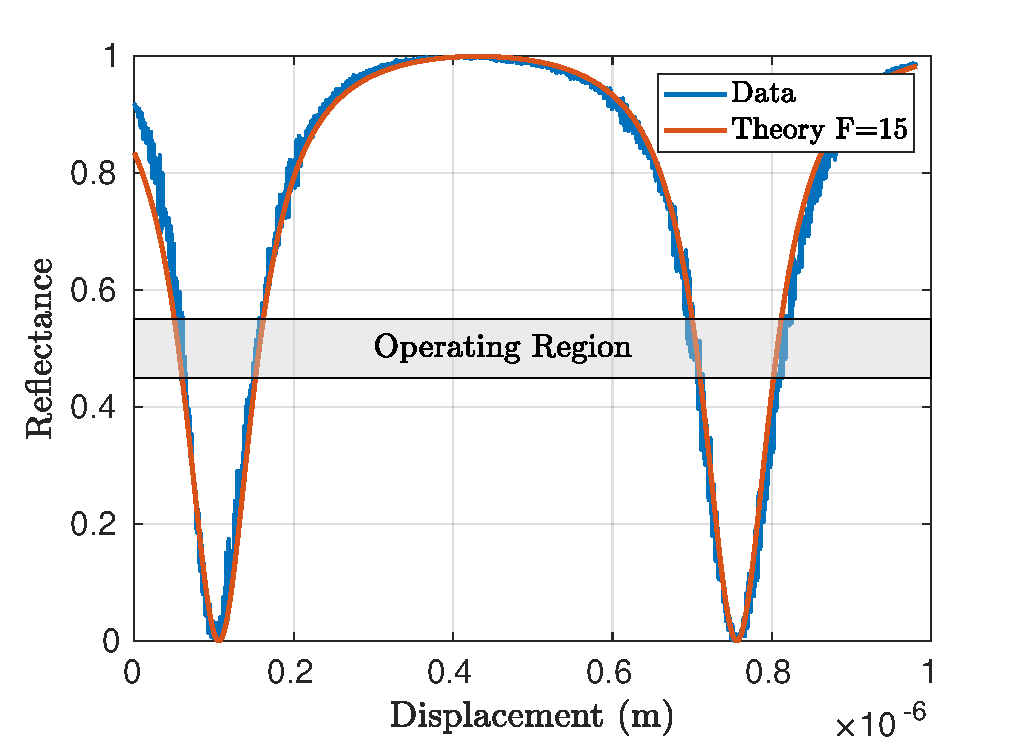
\includegraphics[width=0.75\textwidth]{cBRS_Fringes.pdf}
\caption[Interference pattern of a cBRS fiber interferometer vs cavity length]{Interference pattern of a cBRS fiber interferometer vs cavity length. The gray region is where the device is operated in normal conditions. Within this region the reflectance is approximately linear verse displacement.}
\label{cBRS_fringes}
\end{center}
\end{figure}

This calibration scheme requires independent determination of the wavelength of the laser which is specified by the manufacturer to be 1310 nm$\pm$ 0.01 nm. Additionally, this assumes that the pattern seen at the photodiode is the interference due to the Fabry-Perot cavity formed by the beam splitter coating and the mirror on the beam. This was verified by comparing the refelctance measurements to the theory as can be seen in Figure \ref{cBRS_fringes}.

%\begin{center}
%\begin{tabular}{| c | c |}
%\hline
%Piezo 1 Calibration & 0.672 $\mu$m/V\\
%\hline
%Interferometer 1 Calibration & 23.6 nm/V\\
%\hline
%Piezo 2 Calibration & 0.739 $\mu$m/V\\
%\hline
%Interferometer 2 Calibration& 20.7 nm/V\\
%\hline
%\end{tabular}
%\label{calTable}
%\end{center}

\subsection{Mass Adjustment}

\begin{figure}[!h]
\begin{center}
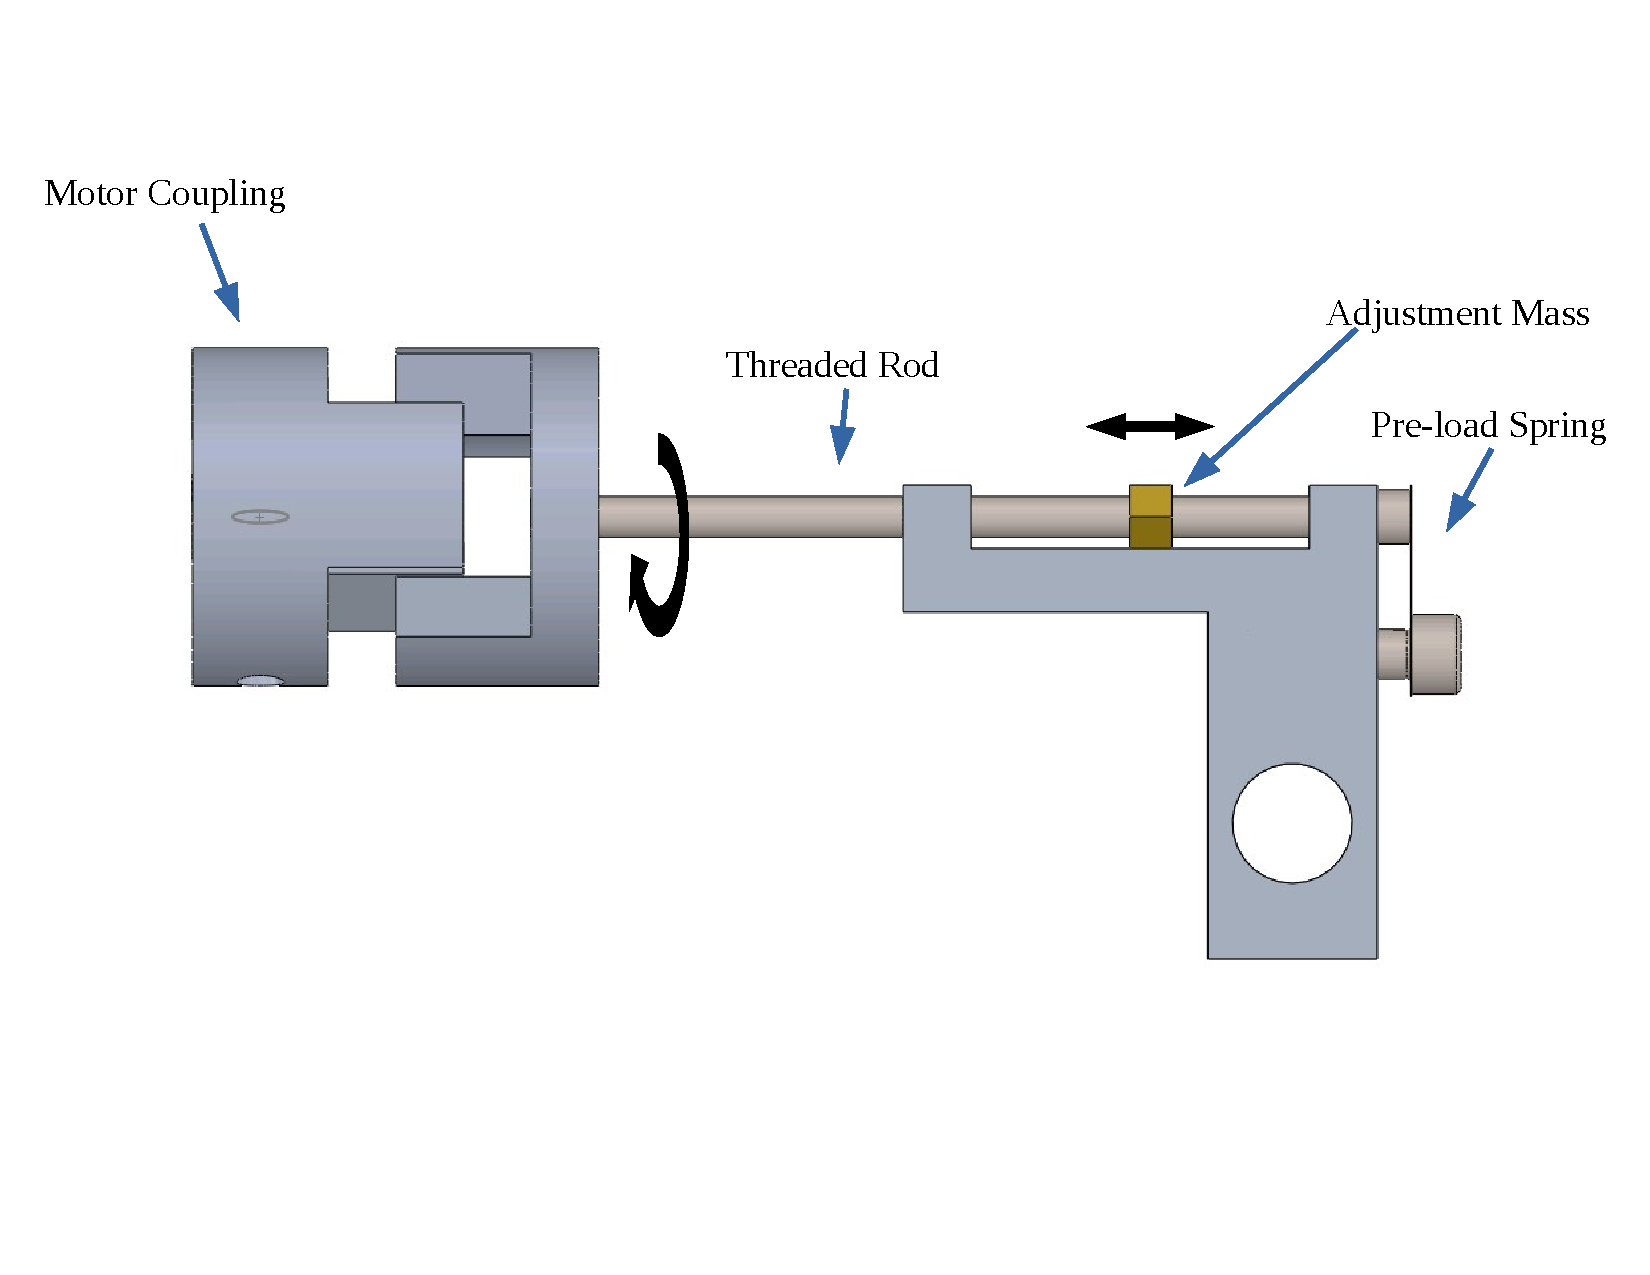
\includegraphics[width=0.85\textwidth]{cBRSMassAdjusterLabeled.pdf}
\end{center}
\caption[CAD rendering of the cBRS mass adjuster]{CAD rendering of the cBRS mass adjuster}\label{massAdjust}
\end{figure}


Through a variety of mechanisms, both the BRSs and the cBRS can undergo long term drifts of the equilibrium position that can drive the beam-balance past the dynamic range of the readout. To counteract this, a mass on the balance can be moved or added to shift the center of mass as follows:
\begin{align}
\Delta \theta=\frac{g}{\kappa} m r
\end{align}
where $\Delta \theta$ is the change in equilibrium angle, $g$ is the gravitational acceleration, $\kappa$ is the spring constant of the flexure, $m$ is the mass added, and $r$ is the distance from the mass and the pivot point.

While for the BRS the horizontal center of mass (COM) was designed to be tuned by hand, for the cBRS to operate within the LIGO vacuum chambers this must be done remotely and in an automated fashion. To achieve this a mass adjuster shown in Figure \ref{massAdjust} consisting of a small brass mass on a fine pitched screw is attached to the beam-balance. This allows the shifting of the mass with the rotation of the screw. 

\begin{figure}[!h]
\begin{center}
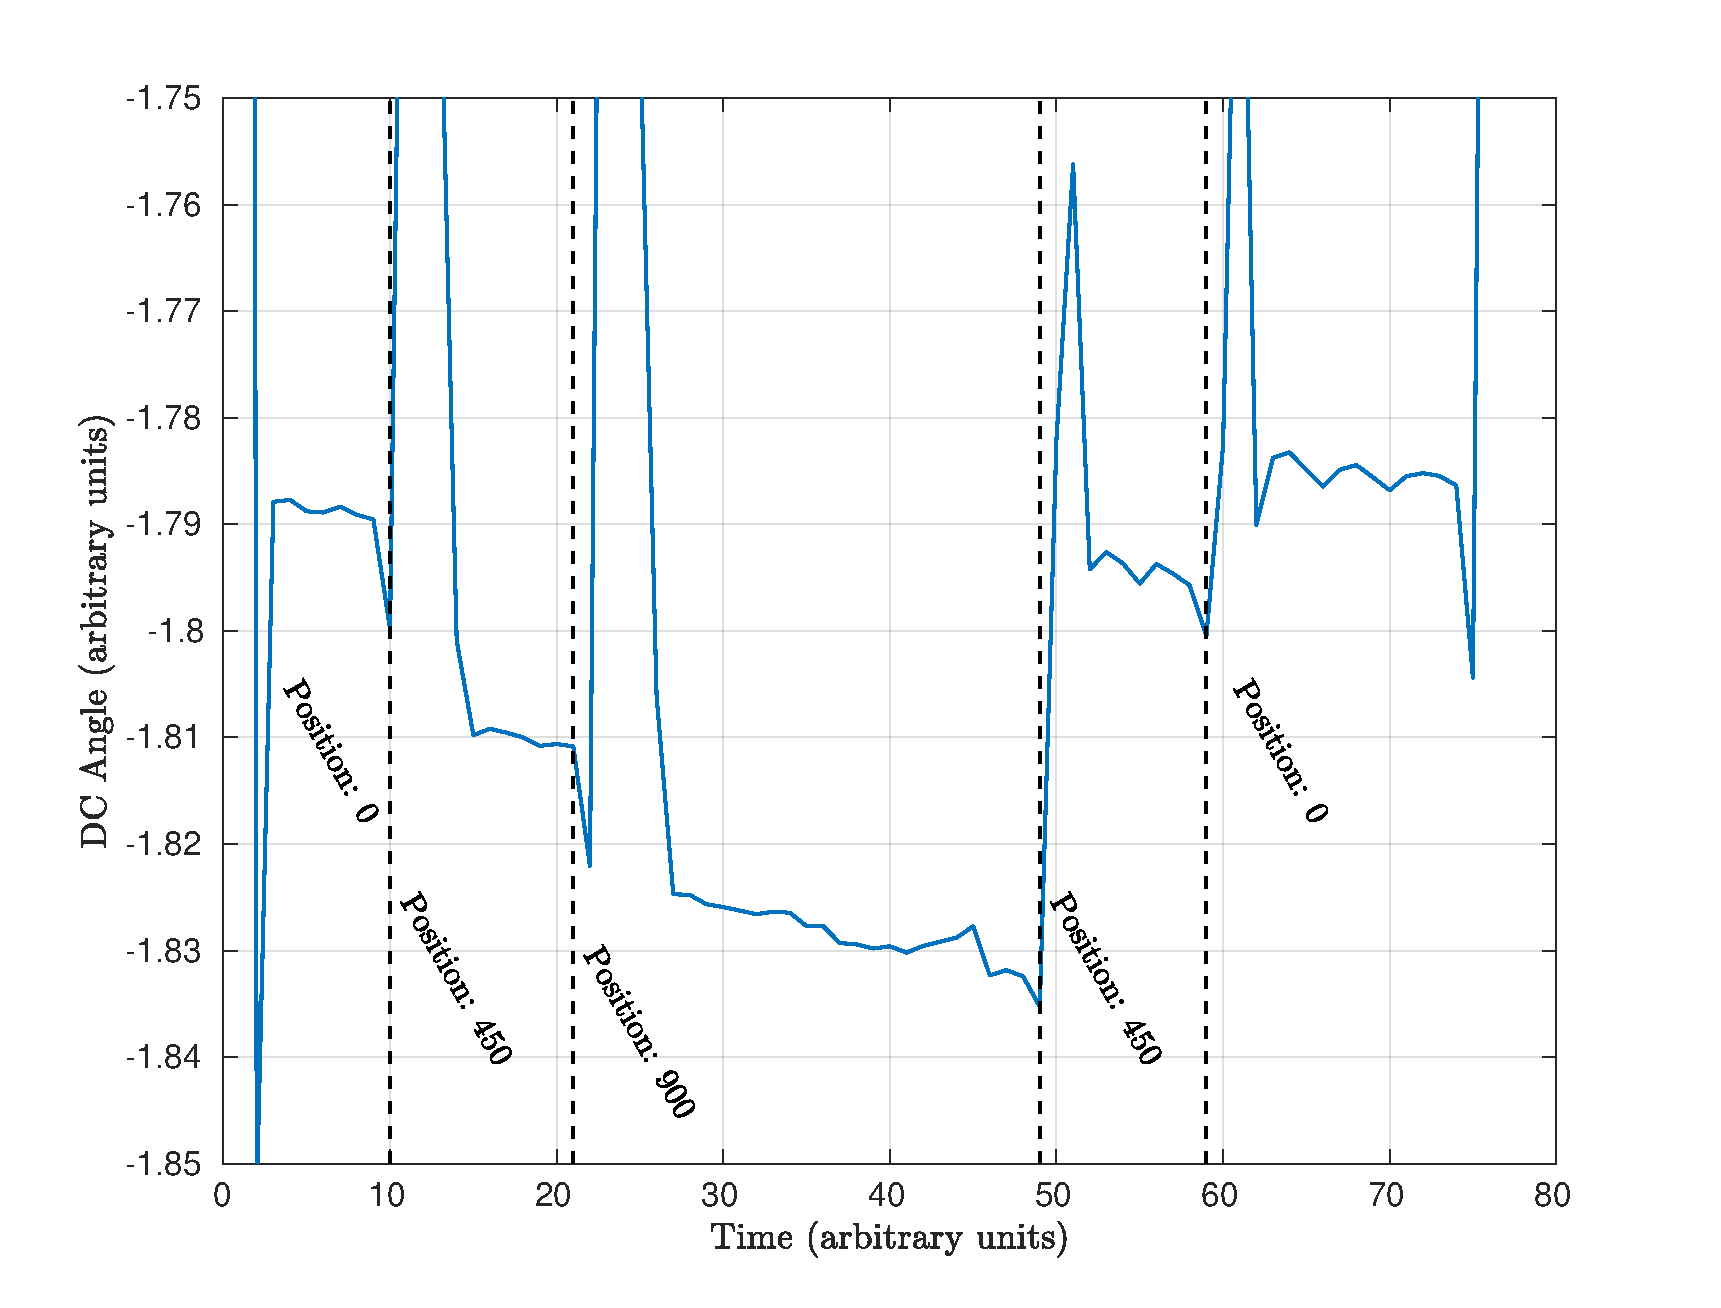
\includegraphics[width=\textwidth]{cBRS_massAdjust.pdf}
\end{center}
\caption[Demonstration of the effect of actuating the remote mass adjuster]{Demonstration of the effect of actuating the remote mass adjuster. The DC angle was measured by taking the mean of period long chunks of shadow sensor data while the mass adjuster was shifted to a collection of positions.}\label{massAdjustPlot}
\end{figure}


In order to avoid mechanically shorting the beam balance with wires, the motor which turns this screw is held on an independent support. The couplers between the motor and the screw are intentially oversized to allow for decoupling via back rotations. A small shim of beryllium copper is held tightly against the opposite end of the screw to provide spring loading which hold the screws center of mass in place but allow for rotation.

To test whether this design was capable of moving enough mass accurately, a temporary uncalibrated shadow sensor was set up to measure the motion of the cBRS. The actuation of the mass adjuster can be seen in Figure \ref{massAdjustPlot} which shows the average of period long cuts of the cBRS's resonant motion. In this prototype there is clear hysteresis due to nonuniform friction along the length of the adjuster. However, this was found to not affect the ability to center the cBRS. 

\subsection{Controls}

Similar to the BRS, the cBRS can be rung up do to environmental transients which can cause resonant motion in excess of the readout's dynamic range. To decrease these amplitudes, two capacitive actuators are placed under the end masses of the beam. These are actuated with low gain with the angular-readout band-passed around the resonant frequency. This allow for low Q motion during high amplitudes and high Q during low amplitudes.

\subsection{Noise Performance}

\begin{figure}[!h]
\begin{center}
 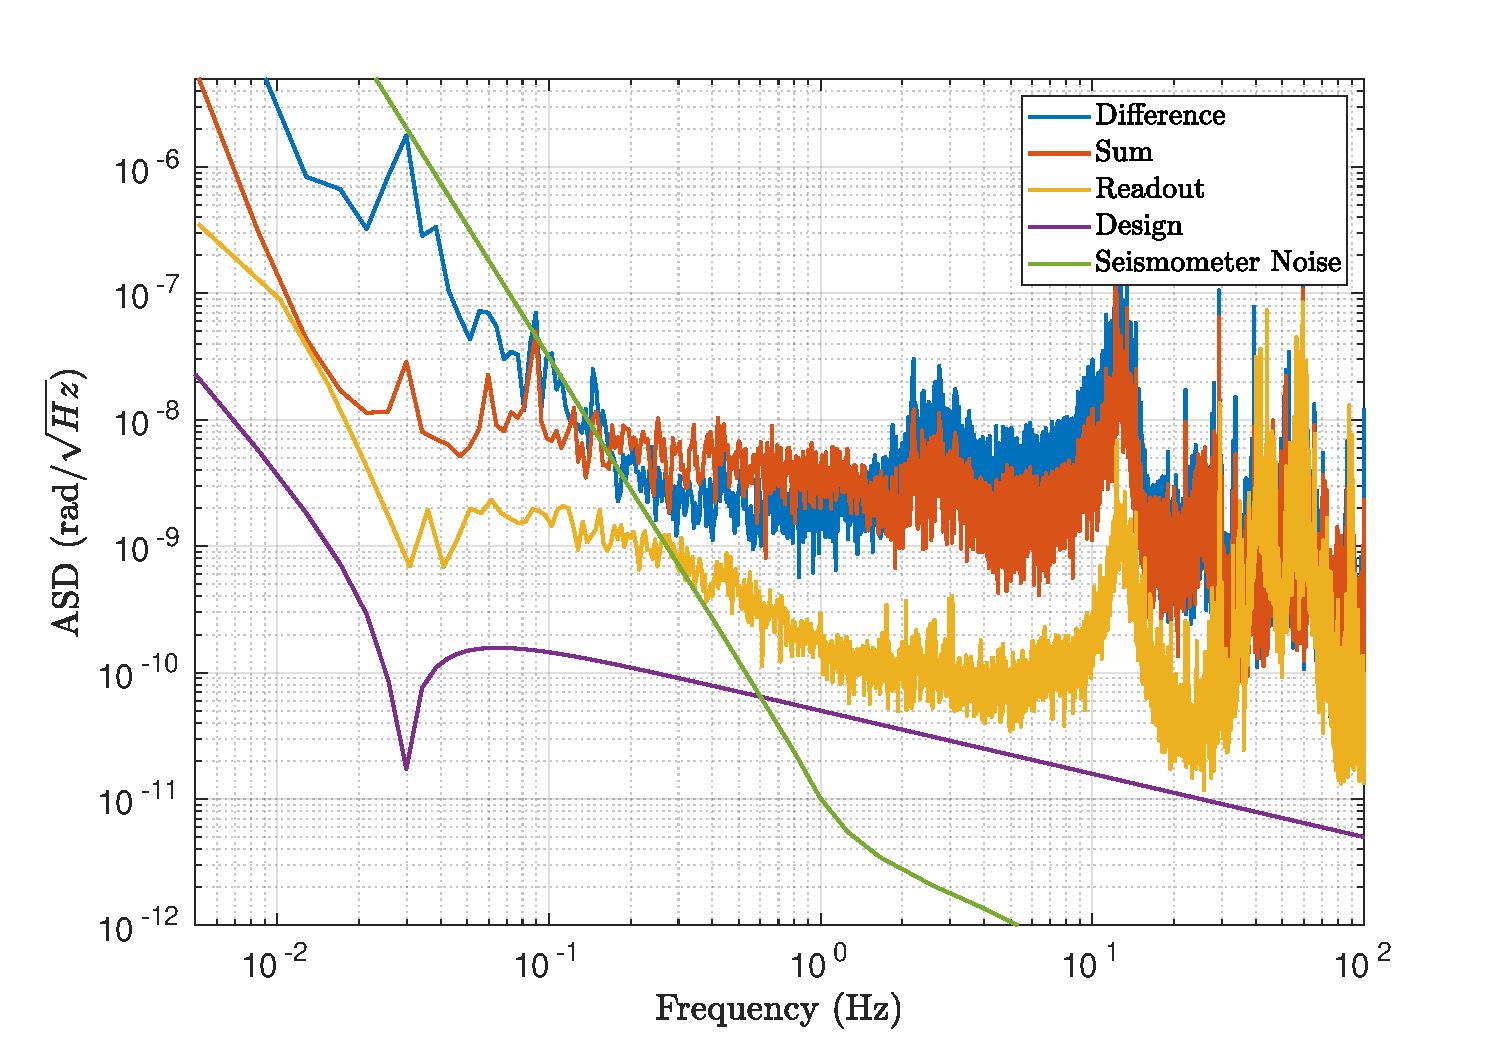
\includegraphics[width=\textwidth]{cBRS_Noise.pdf}
\caption[Prototype cBRS noise performance]{Prototype cBRS noise performance showing the sum and difference of the two readouts. Additionally shown is the readout noise measured while the beam balance was mechanically locked, the design sensitivity, and the sensitivity of the current Stage 2 rotational sensors.}
\label{cBRS_noise}
\end{center}
\end{figure}

The noise performance of the current cBRS prototype, shown in Figure \ref{cBRS_noise} is not as well modeled as the BRS, Section \ref{BRSNoise}, and does not meet the design sensitivity of the instrument. The design sensitivity is determined by extrapolating the high frequency readout noise of 50 prad/$\sqrt{f}$ down to low frequency and inverting the response described by Equation \ref{theta_s}.


\section{Projected Improvements}
\subsection{Isolation Scheme} \label{IsoScheme}

As described in Section \ref{seisIso}, each stage and degree of freedom of the seismic isolation system utilizes a blend of multiple sensors as its feedback signal. These consist of two types of sensors: position sensors which sense differential motion between two stages and inertial sensors which sense the motion relative to an inertial frame. To assess the performance improvements that could be achieved with the addition of a cBRS into the system, a simple two stage, two degree of freedom model was constructed. 

\begin{figure}[!h]
\begin{center}
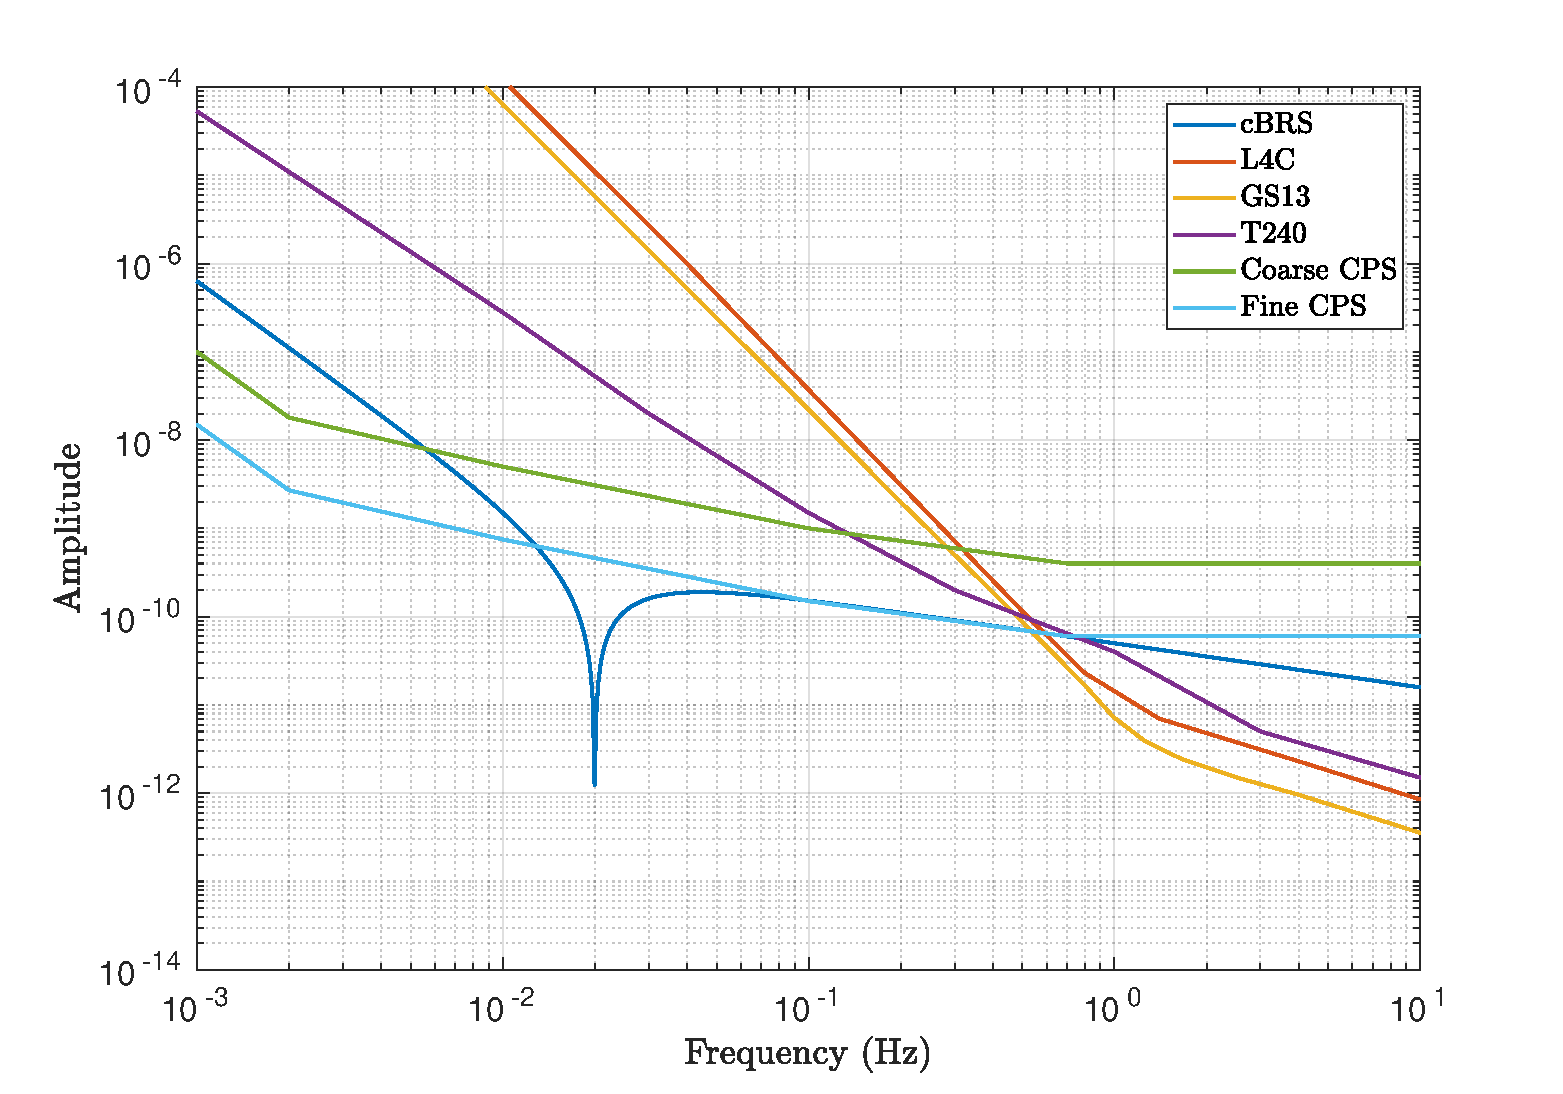
\includegraphics[width=\textwidth]{cBRS_Model_Noise.pdf}
\caption[Noise models for the cBRS, a collection of seismometers, and two types of CPS]{Noise models for the cBRS, a collection of seismometers: L4C, GS13, T240, and two types of CPS: Fine, used between Stage 1 and Stage 2, and course, used between Stage 0 and Stage 1. Each sensors is in its native units, seismometers and CPS in meters and cBRS in radian. Note that a pair of translational sensors located 1~m apart has roughly the same noise levels in both units.}
\label{sensNoise}
\end{center}
\end{figure}

This model assumes both infinite control authority and no dynamics of the isolation platforms. Additionally, purely theoretical models are used for the input motion and the sensor noises. Although a model which accounts for all six degrees of freedom is required to accurately predict the isolation performance, this simplified model is instructive for comparisons of the performance with and without the cBRS. Similar models \cite{windproofing} have been found to match measurements to within a factor of $\sim$2-3.

Throughout this model second-order binomial filters are used as the blend filters. In addition, for each stage the inertial sensor noise is taken to be the minimum of the collection of inertial sensors. Realistically these sensors also require precise blending but the details of this blending is negligible below $\sim$0.5 Hz. Figure \ref{sensNoise} shows the noise curves for each sensor used in this model.


\subsubsection{Stage 2 Rotational}


In order to achieve the lowest suspension point motion, we choose to model a cBRS on the second stage of the isolation. Logistically, this is also the location which currently has enough space to install a device. Due to the rising low frequency noise in the cBRS, tuning where to place the blend frequency becomes a balance of increasing motion at low frequencies and decreasing motion at high and visa versa. The blend frequency was chosen to give a low frequency RMS motion of $\sim$10 nrad$/\sqrt{\text{Hz}}$ which matches the performance without the cBRS, see Figure~\ref{cBRSCompR}. This criteria called for a blend frequency of 12 mHz. The residual tilt for Stage 2 can be approximated by:

\begin{equation}
\theta_2(f)\approx \tilde{F}_{LP2}\ \big(\theta_1(f)+\tilde{n}_\text{CPS-F}(f)\big)+\tilde{F}_{HP2}\ \text{min}\big[\tilde{n}_\text{cBRS}(f),\ \tilde{n}_\text{GS13}(f)\big]
\end{equation}

where $\theta_1$ is the tilt of Stage 1, $\tilde{F}_{LP2}$ and $\tilde{F}_{HP2}$ are respectively the Stage 2 rotational low and high-pass blend filters, $\tilde{n}_\text{CPS-F}$, $\tilde{n}_\text{cBRS}$, and $\tilde{n}_\text{GS13}$ are the rotational sensor noise for the Fine CPS, cBRS, and GS13, respectively. The performance with this loop can be seen in Figure \ref{cBRS2R}. Above $\sim$500 mHz, the performance is dominated by the GS13 noise and from 80 mHz to 500 mHz it is dominated by cBRS noise. Below 80 mHz, the position sensor contributions become dominate which makes the Stage 2 motion almost equivalent to the Stage 1 motion. The only deviation from Stage 1 motion is near the blend frequency, 12 mHz, where gain peaking added a factor of~$\sim$~3. 

\begin{figure}[!h]
\begin{center}
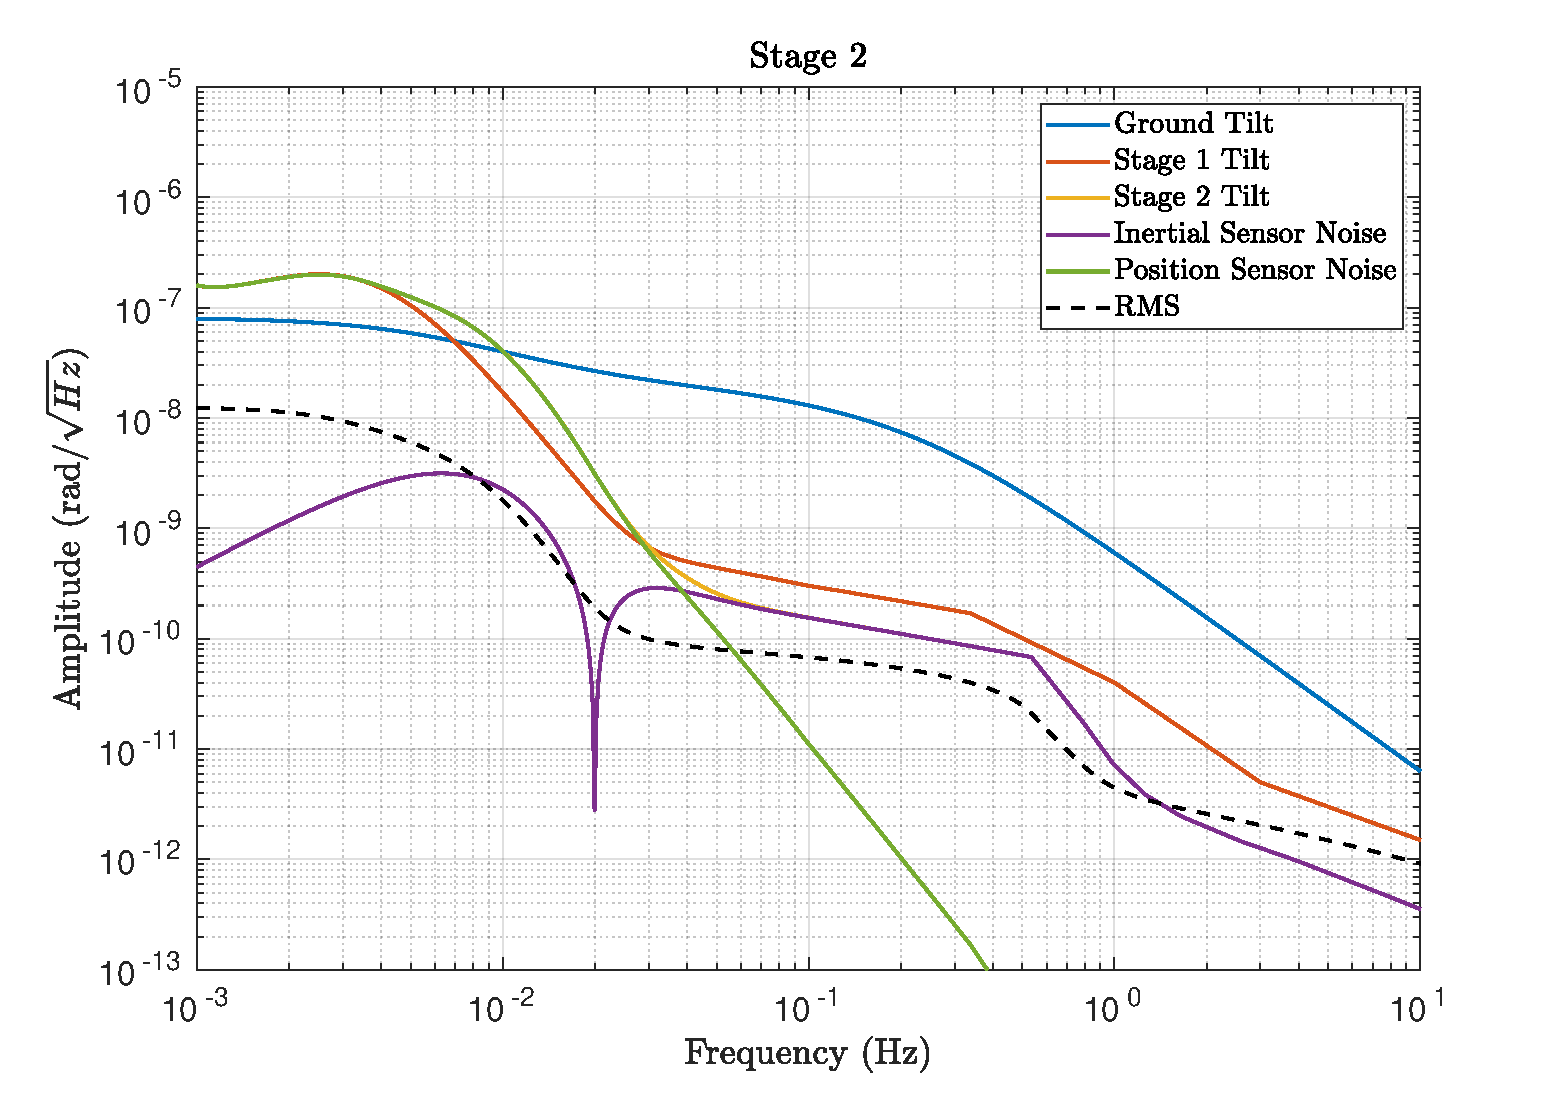
\includegraphics[width=\textwidth]{cBRS_Model_ST2RX.pdf}
\caption[Projected rotational performance of Stage 2 of the ISI]{Projected rotational performance of Stage 2 of the ISI along with the contributions from the inertial and position sensor. Also shown is the input ground tilt model which represents the observed tilt during windy times and the rotational performance of the Stage 1.}
\label{cBRS2R}
\end{center}
\end{figure}

\subsubsection{Stage 1 Rotational}

With Stage 2 inertially isolated in the rotation degree of freedom above $\sim$80 mHz, Stage 1 can achieve superior performance if its control is a combination of the position sensor between the Stage 1 and Stage 2, fine CPS, at high frequencies, and the position sensor between Stage 1 and Stage 0, course CPS, as low. This is effectively using the Stage 2 platform as an inertial proof mass with the fine CPS as a readout. The past scheme was to use a seismometer pair as an inertial rotation sensor for high frequencies and the course CPS at low. Applying the same criteria as Stage 2 of requiring low frequency RMS motion of $\sim$10 nrad$/\sqrt{\text{Hz}}$ yields a blend frequency of 3 mHz around which the motion is amplified by a factor of~$\sim$~3 because of gain peaking. 

\begin{figure}[!h]
\begin{center}
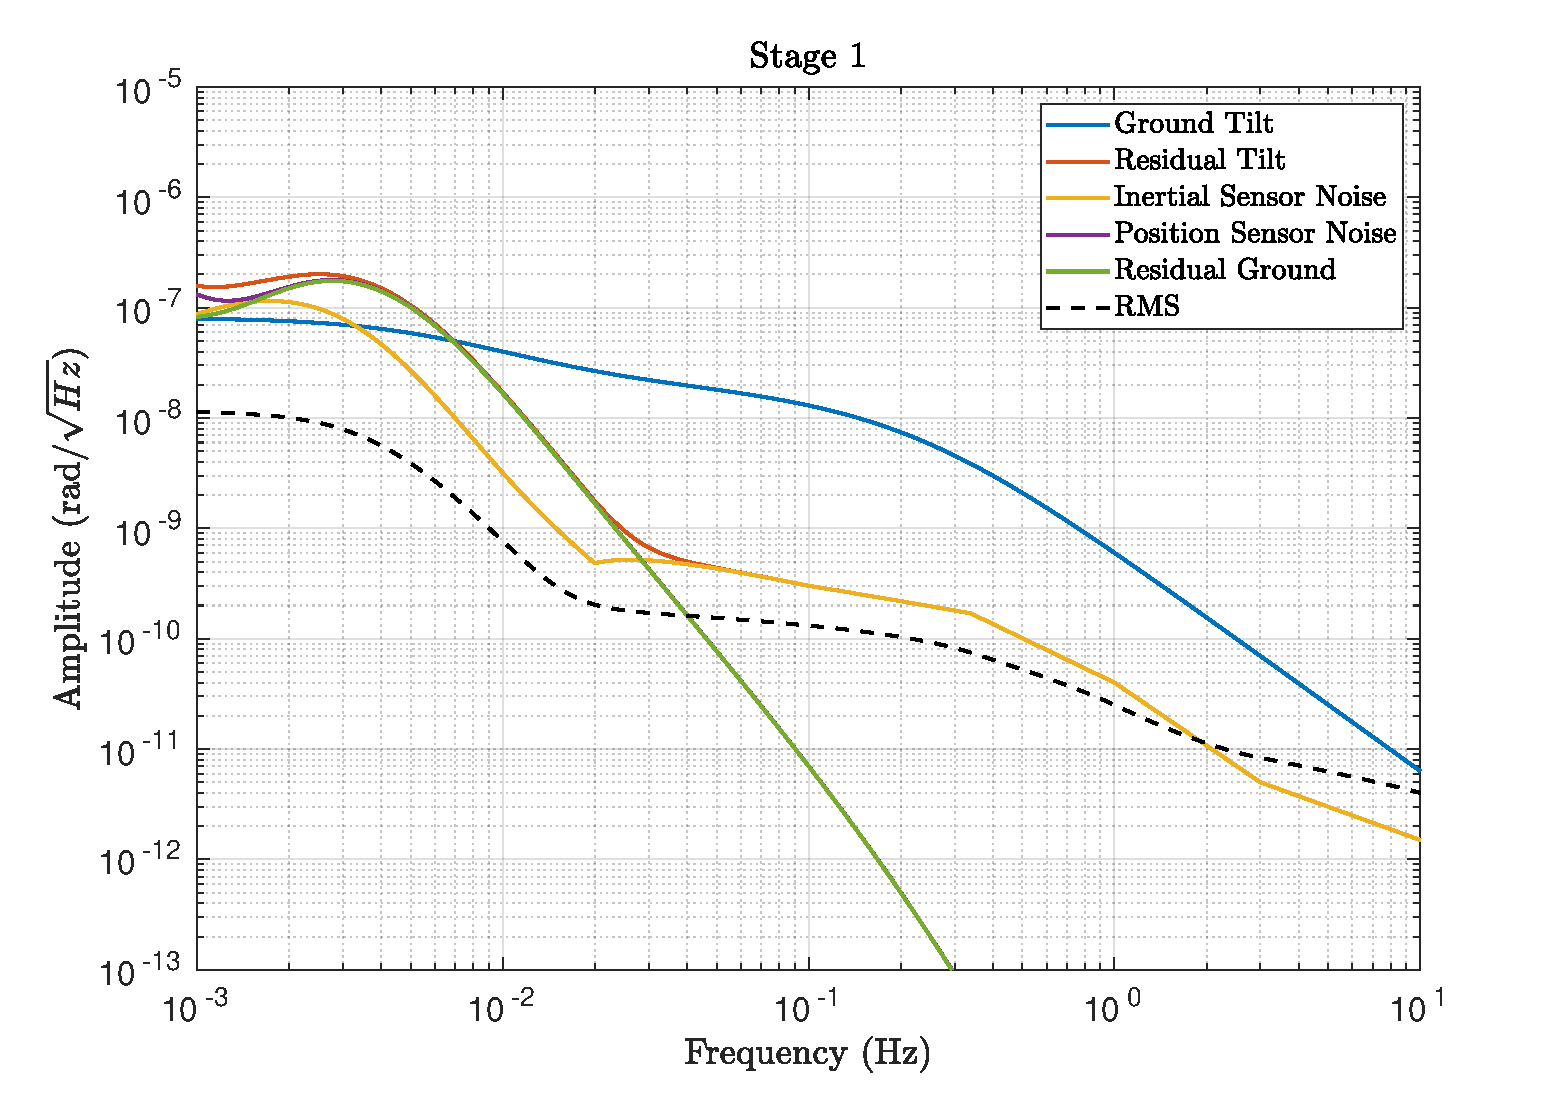
\includegraphics[width=\textwidth]{cBRS_Model_ST1RX.pdf}
\caption[Projected rotational performance of Stage 1 of the ISI]{Projected rotational performance of Stage 1 of the ISI with, yellow, and without, red, the cBRS. Also shown is the input ground tilt model, blue, which represents the observed tilt during windy times.}
\label{cBRS1R}
\end{center}
\end{figure}

The residual tilt for Stage 1 can be approximated by:

\begin{equation}
\theta_1(f)\approx \tilde{F}_{LP1}\ \big(\theta_g(f)+\tilde{n}_\text{CPS-C}(f)\big)+\tilde{F}_{HP1}\ \text{min}\big[(\tilde{n}_\text{cBRS}(f)+\tilde{n}_\text{CPS-F}(f)),\ \tilde{n}_\text{T240}(f)\big]
\end{equation}

where $\theta_g$ is the ground tilt, $\tilde{F}_{LP1}$ and $\tilde{F}_{HP1}$ are respectively the Stage 1 rotational low and high-pass blend filters, $\tilde{n}_\text{CPS-C}$, $\tilde{n}_\text{CPS-F}$, $\tilde{n}_\text{cBRS}$, and $\tilde{n}_\text{T240}$ are the rotational sensor noise for the Course CPS, Fine CPS, cBRS, and T240, respectively.

The performance of this design can be seen in Figure~\ref{cBRS1R} Below 1 mHz, it is expected the platform motion follows the ground. However, this is omitted as both the ground rotation and sensor noise are not well constrained at low frequency. Above $\sim$30 mHz, the residual is dominated by the combination of the sensor noises from the fine CPS, from 30 mHz to 350 mHz, and the T240 pair, above 350 mHz.

A subtly that arises from using both the fine and course CPS as the control for Stage 1 is that if the Stage 2 blend frequency is placed below the Stage 1 frequency then in between these two frequencies both stages are using the fine CPS as their control. Since the fine CPS measures the motion between the two stages, this effectively makes both stages uncontrolled as they are not referenced to any independent frame. In our model this is avoided by placing the Stage 1 blend frequency a decade lower than the Stage 2 blend.

\subsubsection{Stage 1 Translational}

Once the rotational degrees of freedom are controlled, the translational loops can begin to be tuned. The primary dependence of the traslational performance on the rotational performance comes from tilt contamination of seismometers, described in Section \ref{tiltCon}. As with the rotational control loop design, the choice of blend frequency is a trade off between increasing low frequency motion and decreasing high. We choose to require low frequency RMS performance of $<$ 100 nm/s$/\sqrt{\text{Hz}}$. This requirement is approximately the performance of the current seismic isolation system. A blend frequency of 15 mHz was found to exceed this requirement. The residual motion for Stage 1 can be approximated by:

\begin{equation}
x_1(f)\approx F_{LP1}\ \big(x_g(f)+n_\text{CPS-C}(f)\big)+F_{HP1}\ \big( g/\omega^2\ \theta_1(f) +n_\text{T240}(f) \big)
\end{equation}

where $x_g$ is the ground motion, $F_{LP1}$ and $F_{HP1}$ are respectively the Stage 1 translational low and high-pass blend filters, and $n_\text{CPS-C}$ and $n_\text{T240}$ are the translational sensor noise for the Course CPS and T240, respectively.

The performance of the Stage 1 translational isolation with this choice can be seen in Figure \ref{cBRS1X}. Above 500 mHz, the performance is limited by the T240 noise. Between 25-500 mHz, residual ground motion dominates and between 1-25 mHz residual tilt coupled through tilt contamination of the seismometers is the primary contribution. 

\begin{figure}[!h]
\begin{center}
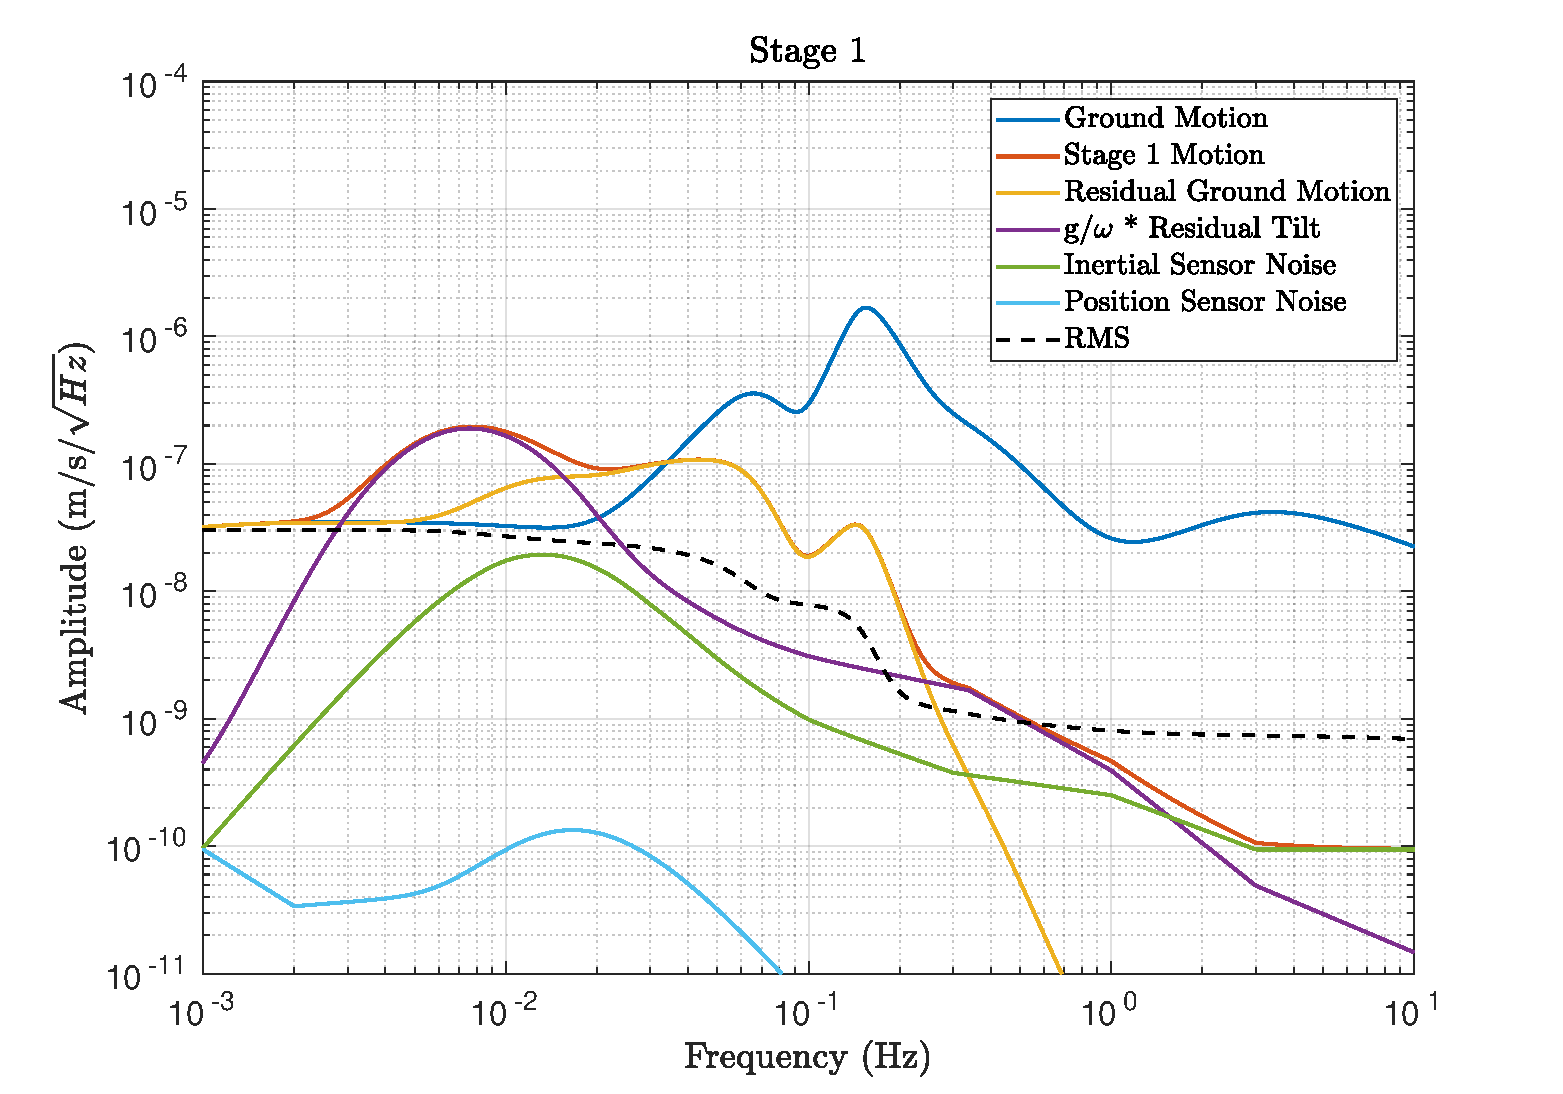
\includegraphics[width=\textwidth]{cBRS_Model_ST1X.pdf}
\caption[Projected translational performance of Stage 1 of the ISI]{Projected translational performance of Stage 1 of the ISI with, yellow, and without, red, the cBRS. Also shown is the input ground motion model, blue, which represents the observed tilt during windy times. The control loops here can be tuned to decrease motion at $\sim$100 mHz, the microseism frequencies, by increasing motion at $\sim$10 mHz and vice versa.}
\label{cBRS1X}
\end{center}
\end{figure}

\subsubsection{Stage 2 Translational}

\begin{figure}[!h]
\begin{center}
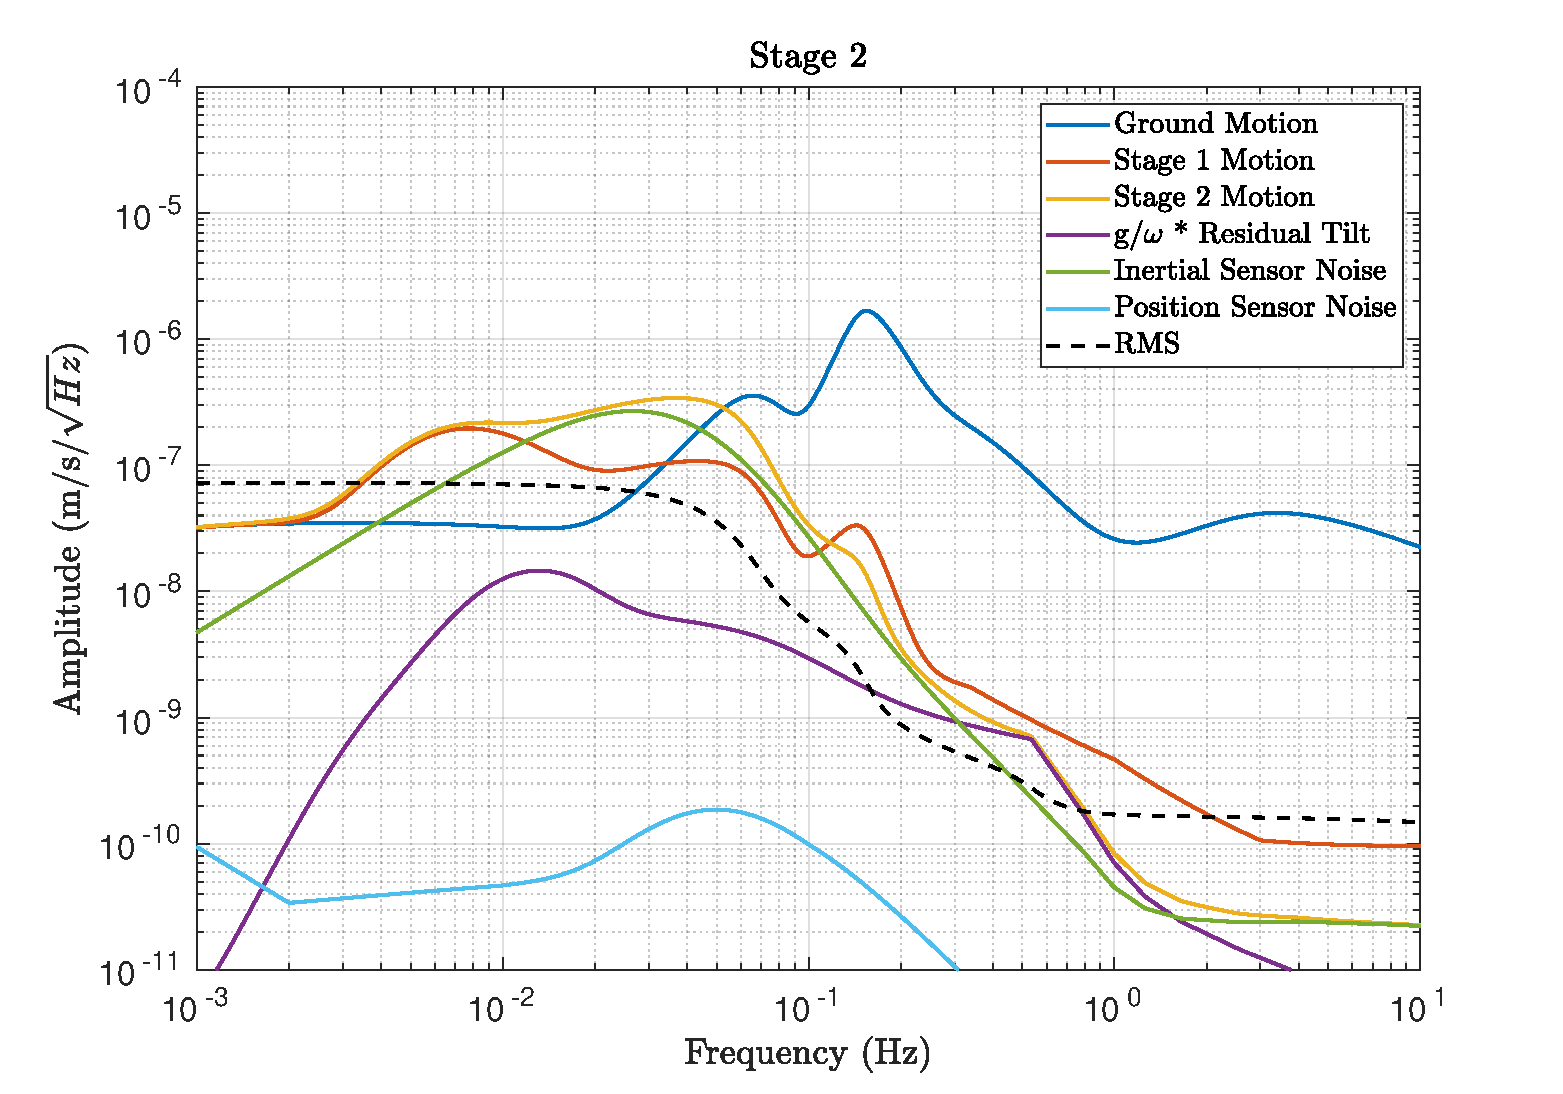
\includegraphics[width=\textwidth]{cBRS_Model_ST2X.pdf}
\caption[Projected translational performance of Stage 2 of the ISI] {Projected translational performance of Stage 2 of the ISI with, yellow, and without, red, the cBRS. Also shown is the input ground motion model, blue, which represents the observed tilt during windy times. The control loops here can be tuned to decrease motion at $\sim$100 mHz, the microseism frequencies, by increasing motion at $\sim$10 mHz and vice versa.}
\label{cBRS2X}
\end{center}
\end{figure}
The Stage 2 translational loops were tuned in a similar manner as Stage 1: requiring that the RMS motion at 1 mHz to be $<$ 100 nm/s$/\sqrt{\text{Hz}}$. This yielded  a blend frequency of 45 mHz. The residual motion for Stage 2 can be approximated by:

\begin{equation}
x_2(f)\approx F_{LP2}\ \big(x_1(f)+n_\text{CPS-F}(f)\big)+F_{HP2}\ \big( g/\omega^2\ \theta_2(f) +n_\text{GS13}(f) \big)
\end{equation}

where $F_{LP2}$ and $F_{HP2}$ are respectively the Stage 2 translational low and high-pass blend filters, and $n_\text{CPS-F}$ and $n_\text{GS13}$ are the translational sensor noise for the Fine CPS and GS13, respectively.

As can be seen in Figure \ref{cBRS2X}, this effectively flattens the residual spectrum between $\sim$5-60 mHz to an amplitude of 2-3 $\times 10^{-7}$ m/s$/\sqrt{\text{Hz}}$ while decreasing the microseism at 150 mHz by a factor of $\sim$100.

Of particular interest for future upgrades to the seismic isolation, the limiting term of the Stage 2 translational performance in these models is the noise due to the on-platform inertial sensors whereas previous performance was dominated by the tilt contamination term. \cite{windproofing} This points to the need of lower noise inertial sensors for future systems. This is an active area of research with many promising candidate sensors \cite{Mow_Lowry_2019, Cooper_2018}. 

\subsubsection{Comparison with past performance}

To show the improvements relative to the past isolation configurations, the performance of the past isolation system was modeled using the same techniques as described in Section \ref{IsoScheme}. The filters used here were those that were deployed for O2. These are expertly tuned to account for the true performance of the instruments and thus have more complex shapes than the binomial filters used in the proposed isolation scheme. However, they follow the same general shape as binomial filters.

\begin{figure}[!h]
\begin{center}
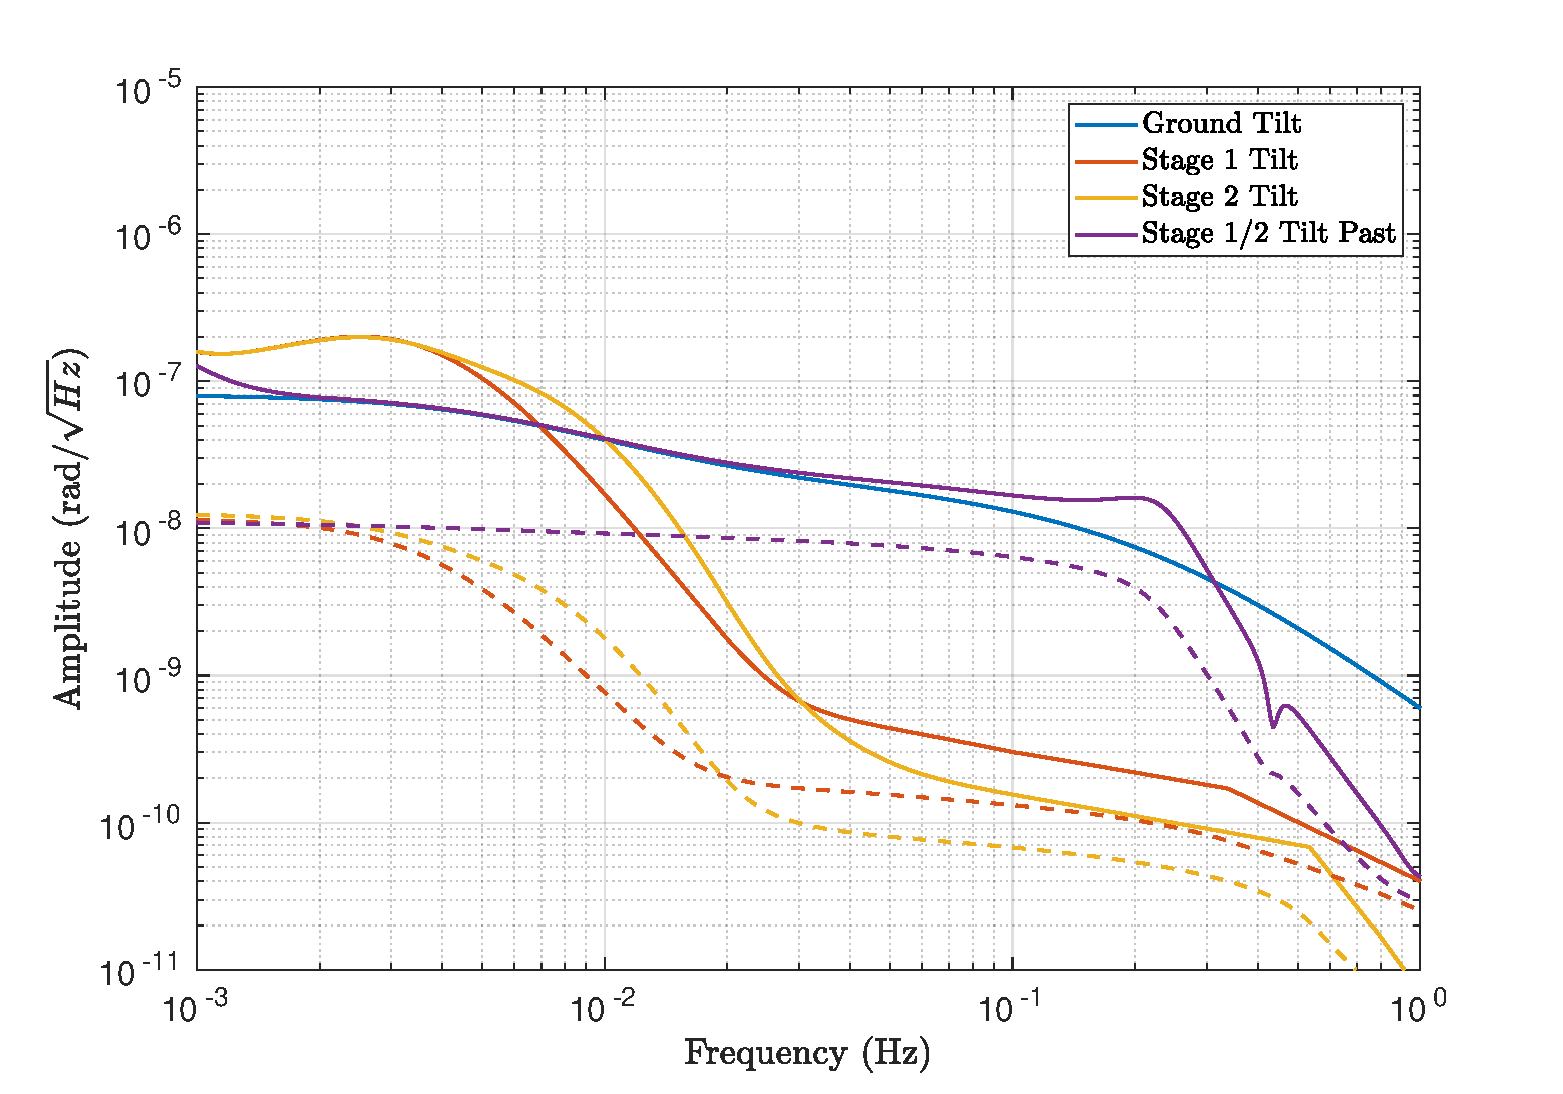
\includegraphics[width=\textwidth]{cBRS_Model_CompRX.pdf}
\caption[Comparison of the rotational isolation performance of Stage 2 during O2 and the projected performance with the inclusion of the cBRS]{Comparison of the rotational isolation performance of Stage 2 during O2 and the projected performance with the inclusion of the cBRS. During O2, the rotational performance of the two stages was identical since they were locked together using the position sensors.}
\label{cBRSCompR}
\end{center}
\end{figure}

A comparison of the rotational degree is shown in Figure \ref{cBRSCompR}. During O2, Stage 2 was locked to Stage 1 in the rotational degree of freedom using the position sensors across the entire band of interest. Thus the performance of the two stages was identical. With the addition of the cBRS the residual tilt is decreased by a factor of $\sim$50 and $\sim$100 respectively for Stage 1 and Stage 2 between 50-250 mHz. Between 1-10 mHz the residual tilt is increased by a factor of $\sim$3. Below 1 mHz it is expected that the two schemes have identical performance. However, the ground tilt is not well modeled due to the lack of sub-mHz rotation sensors so this is omitted from this model.


\begin{figure}[!h]
\begin{center}
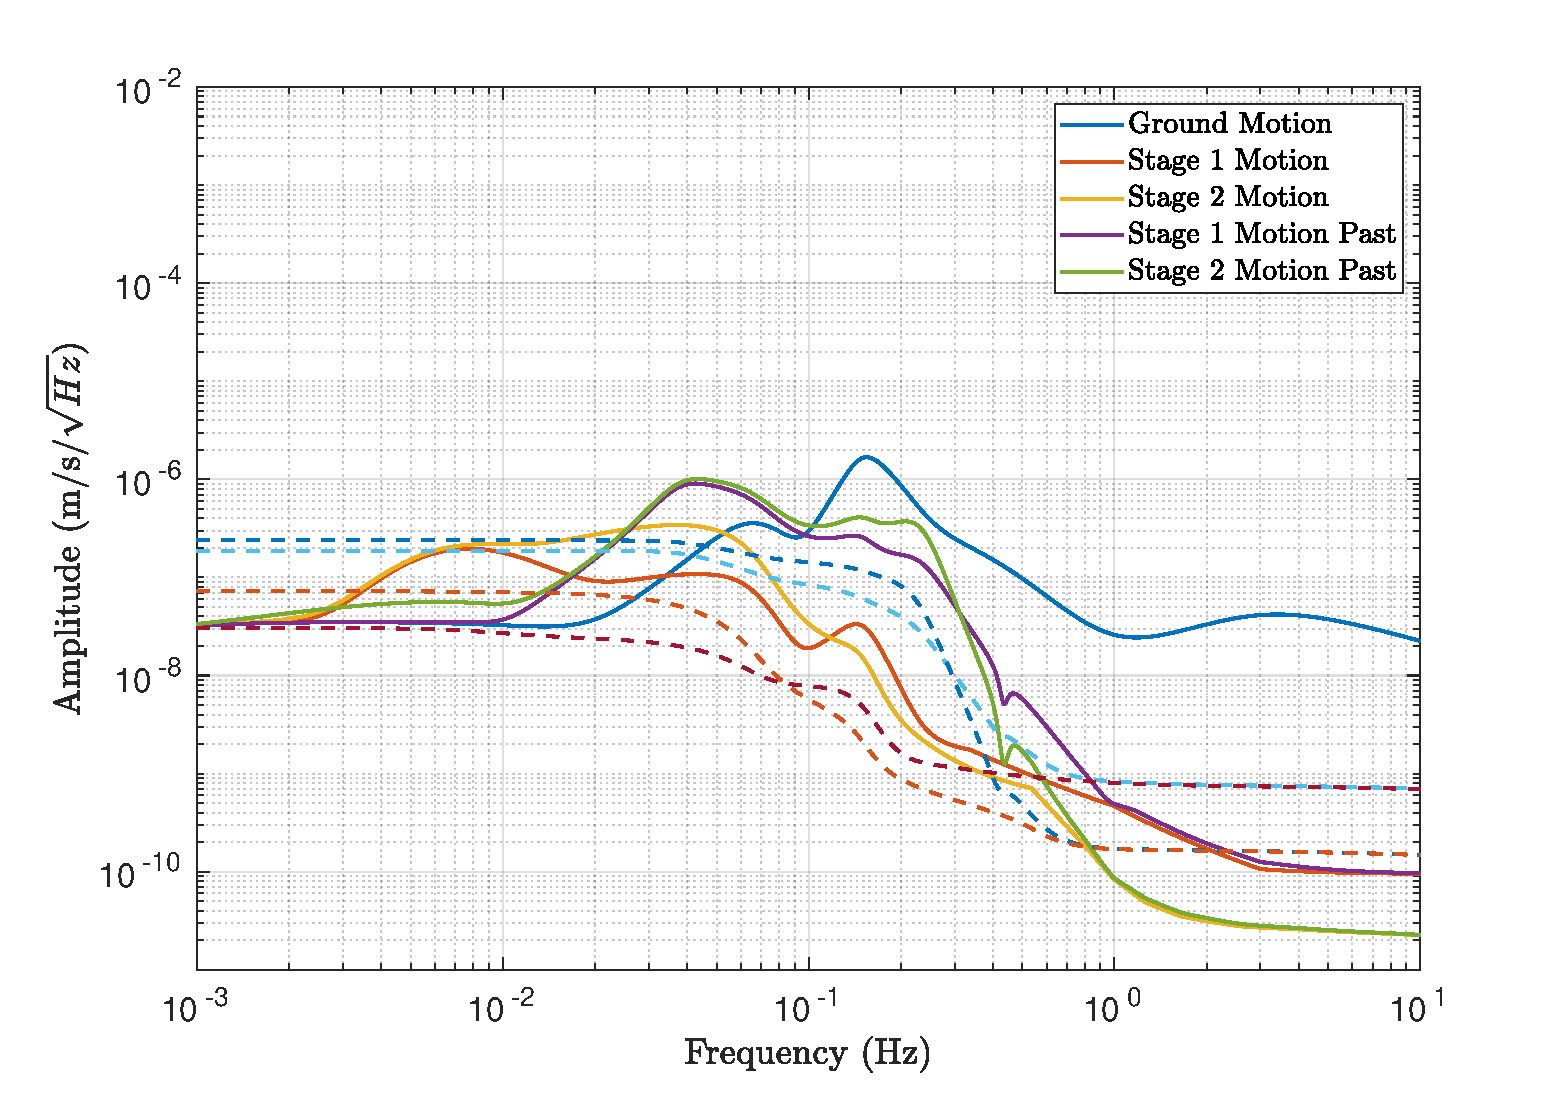
\includegraphics[width=\textwidth]{cBRS_Model_CompX.pdf}
\caption[Comparison of the translational isolation performance during O2 and the projected performance with the inclusion of the cBRS]{Comparison of the translational isolation performance during O2 and the projected performance with the inclusion of the cBRS.}
\label{cBRSCompX}
\end{center}
\end{figure}

The performance comparison of the translational degree isolation system is shown in Figure \ref{cBRSCompX}. Above 1 Hz, the performance of the two schemes are similar as lowest noise sensors at those frequencies have not changed. At the secondary microseism, 100-500 mHz, the inclusion of the cBRS yields a factor of $\sim$20 improvement of the residual motion while at the primary microseism, 50-100 mHz, it yields a factor of $\sim$3. With the cBRS, the residual motion between 3-30 mHz is increased by a factor of ten. However, the RMS motion at those frequencies is still below the previous performance. It is expected that the control loops downstream will be able to compensate for this increase in motion without any decrease in performance. Below 2 mHz, both schemes follow the ground since the dominate sensors at those frequencies are the position sensors.

Although in reality the control loop for each isolation platform will have to be tuned individually, these models show that one can expect a significant decrease in residual motion with the deployment of the cBRS.

\subsection{Angular Control Performance}

\begin{figure}[!h]
\begin{center}
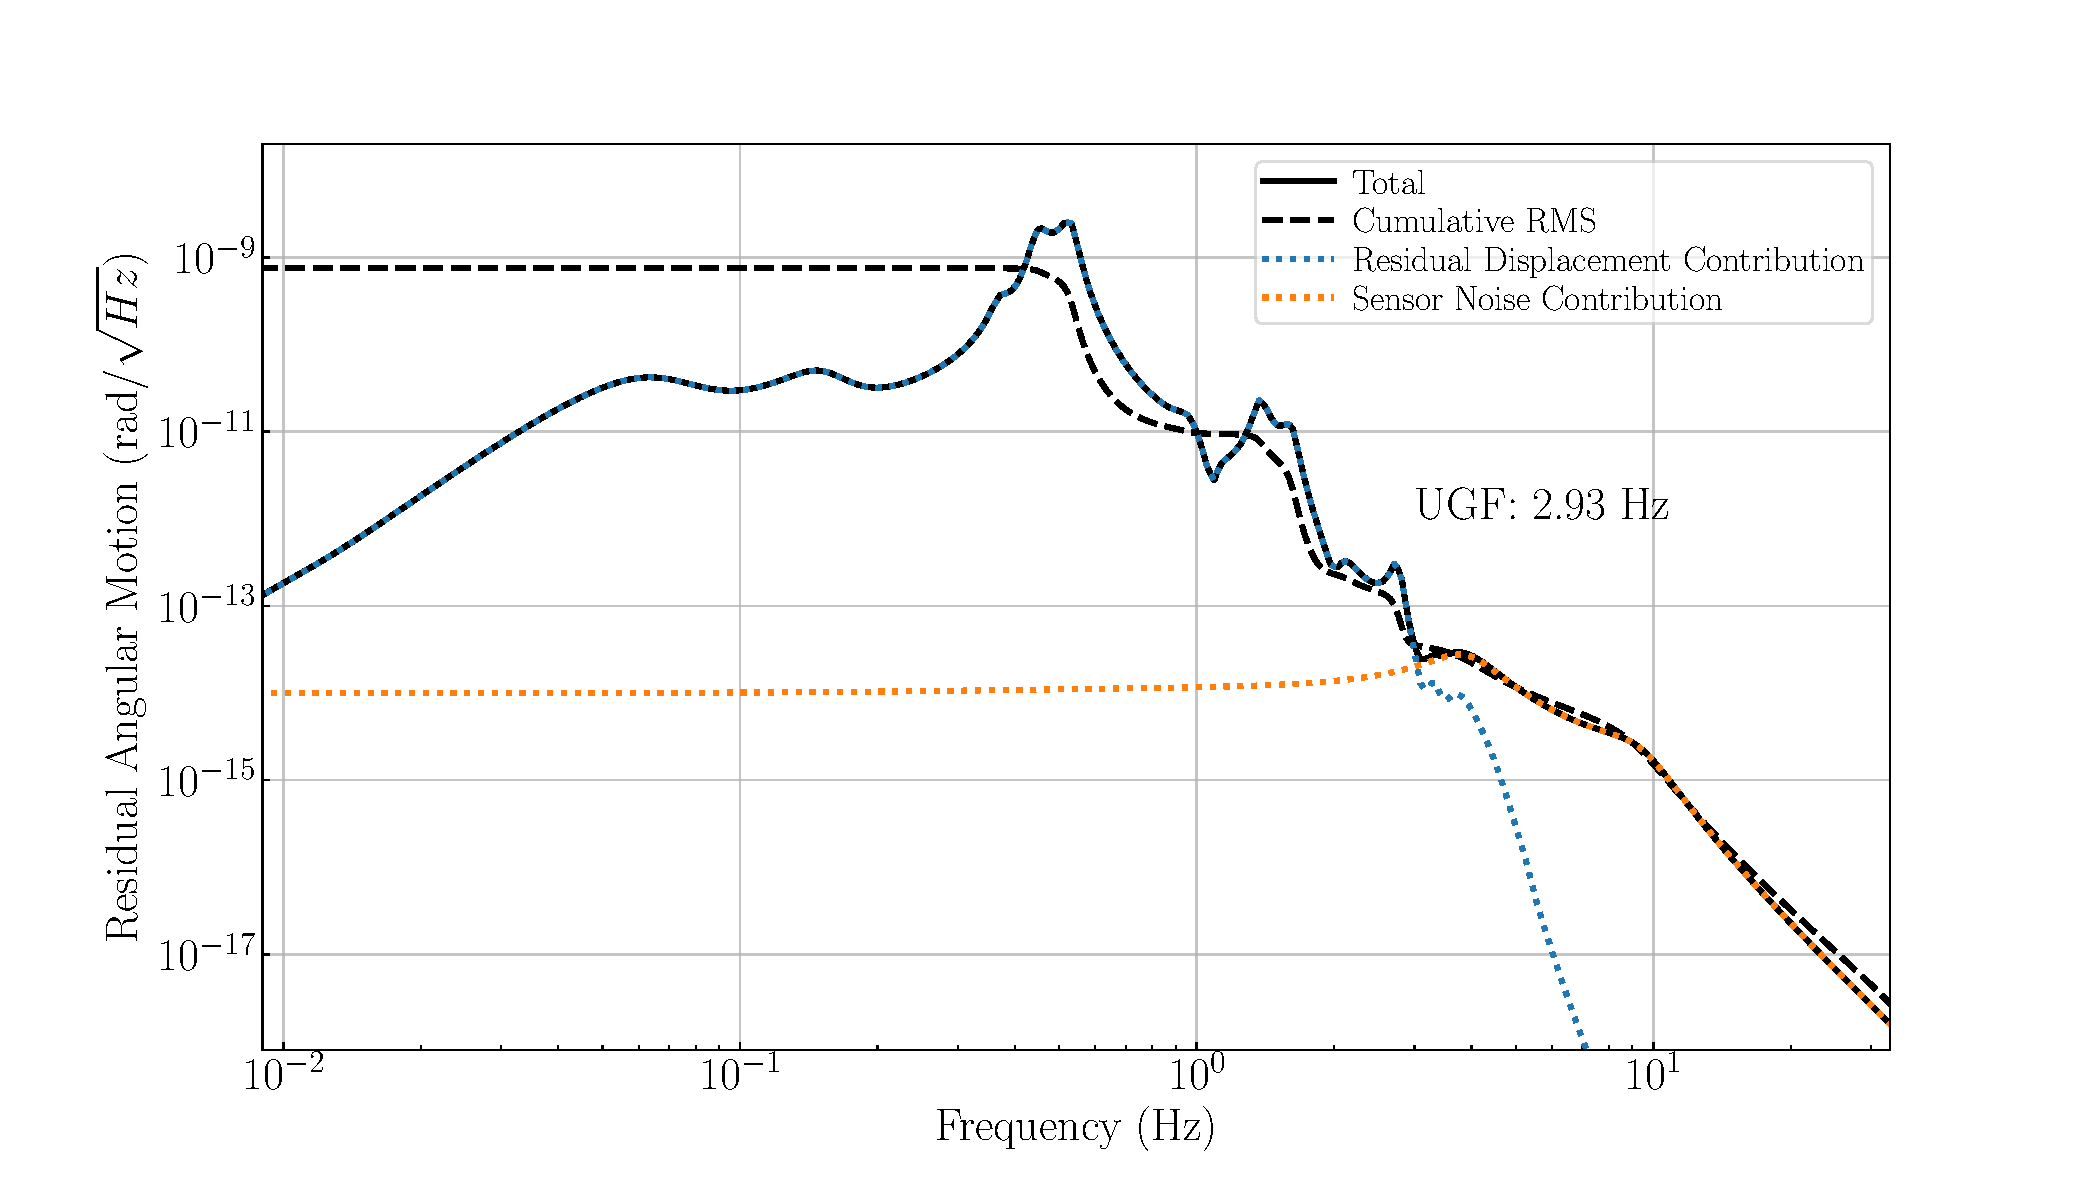
\includegraphics[width=\textwidth]{cBRS_ASC_With.pdf}
\caption[Projected performance of the angular sensing and control system]{Projected performance of the angular sensing and control system with the seismic performance described in Section \ref{IsoScheme}.}
\label{ascWith}
\end{center}
\end{figure}

As mentioned in Section \ref{ASC}, the most immediate effect of the increased performance of the seismic isolation with the inclusion of a cBRS is the ability to retune the angular sensing and control (ASC) loops. In order to estimate the possible ASC performance for a given seismic performance, a simplified model was constructed which takes the motion of the suspension point as an input, optimizes a theoretical control loop, and outputs the expected residual angular motion of the test mass. The control loop is optimized to give the best performance at high frequencies while maintaining a low frequency RMS residual of 1 nrad/$\sqrt{\text{Hz}}$.

This model uses a handful of approximations that do not neccessarily hold in reality. First off, this is only modeling the performance of a single test mass yet to predict the effect on the differential strain, all four test masses would need to be modeled. Additionally, it ignores the effects of radiation pressure which become important at high laser powers. \cite{ASC} However, it is believed that the seismic isolation performance at low frequencies is the limiting factor in the current observatories and thus is captured by this model. 

The performance of the ASC system was modeled for both the seismic performance with, Figure \ref{ascWith}, and without, Figure \ref{ascWithout}, the cBRS installed. In both situations, the high frequency performance is limited by sensor noise which leaks into the gravitational wave band. The primary retuning that can be made with the inclusion of the cBRS is to decreasing the ASC UGF from 5.23 Hz to 2.93 Hz. Above this the residual falls off as 1/$f^5$.

\begin{figure}[!h]
\begin{center}
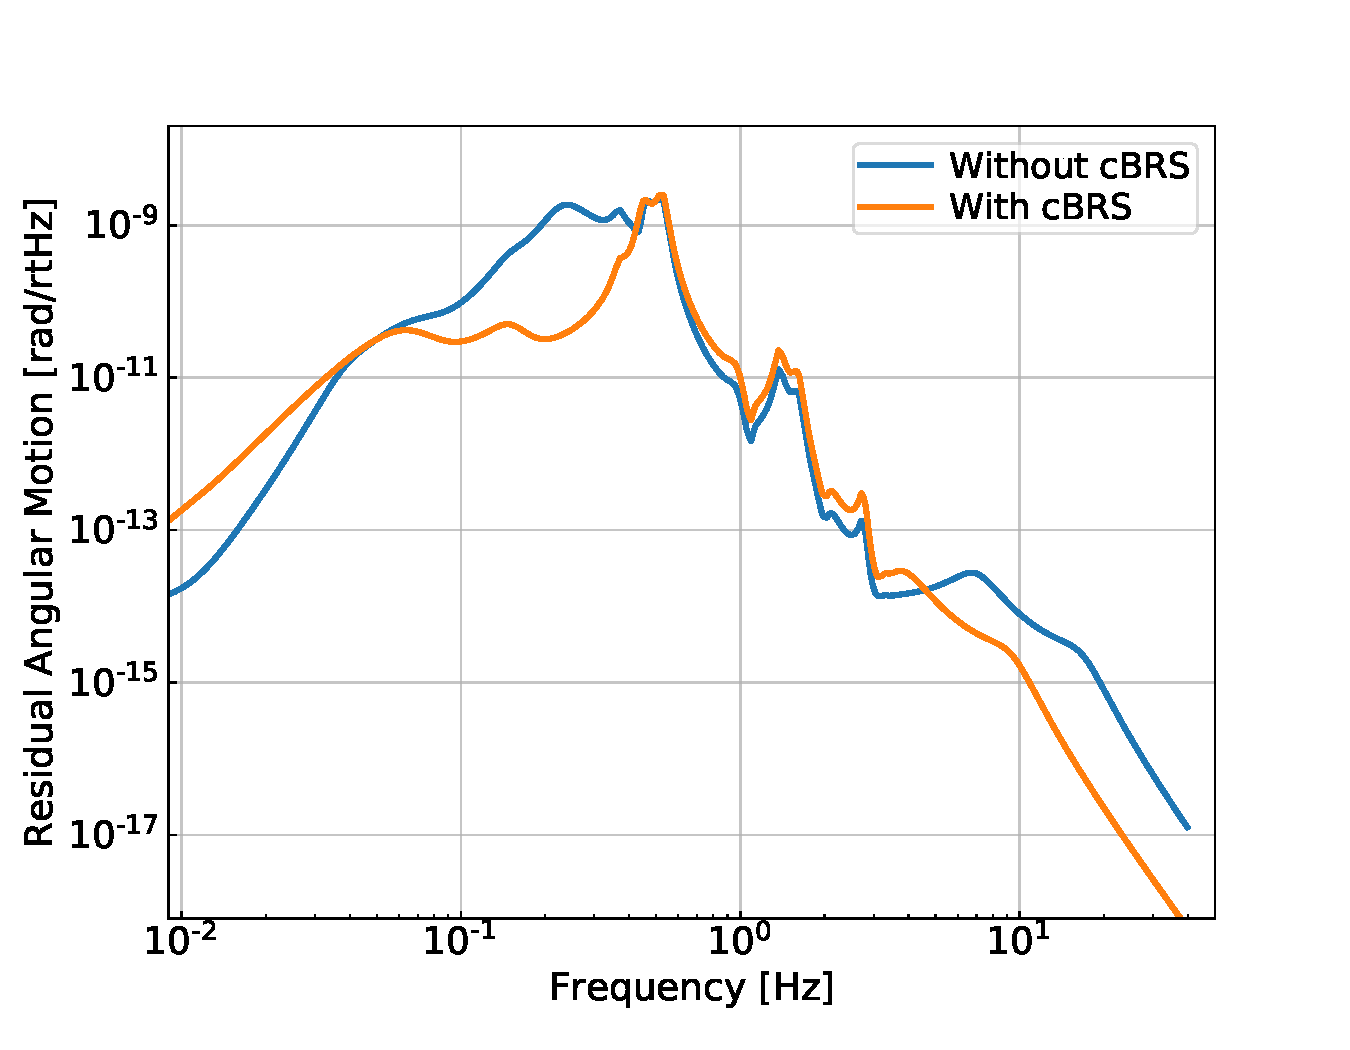
\includegraphics[width=\textwidth]{cBRS_ASC_LowF.pdf}
\caption[Comparison of the ASC performance with and without the cBRS]{Comparison of the ASC performance with and without the cBRS}
\label{ascComp}
\end{center}
\end{figure}

A comparison of the modeled residual for a system with and without the cBRS is shown in Figure \ref{ascComp}. As expected, adding the cBRS reduces the residual between $\sim$50-500 mHz due to the increased performance of the seismic isolation system. This allows a shift in the UGF to lower frequencies which reduces the residual above $\sim$5 Hz. 

This decrease in residual motion above $\sim$5 Hz would directly decrease noise in the differential strain readout of the observatory as shown in Figure \ref{ascStrain}. It should be stressed that for an accurate prediction of the strain noise, one would need to include the contributions from all four test masses and their couplings due to radiation pressure. However, this model suggests that with the future installation of the cBRS one would expect roughly an order of magnitude reduction in the low frequency noise in the gravitational wave channel bringing the noise closer to the aLIGO design sensitivity.

\begin{figure}[!h]
\begin{center}
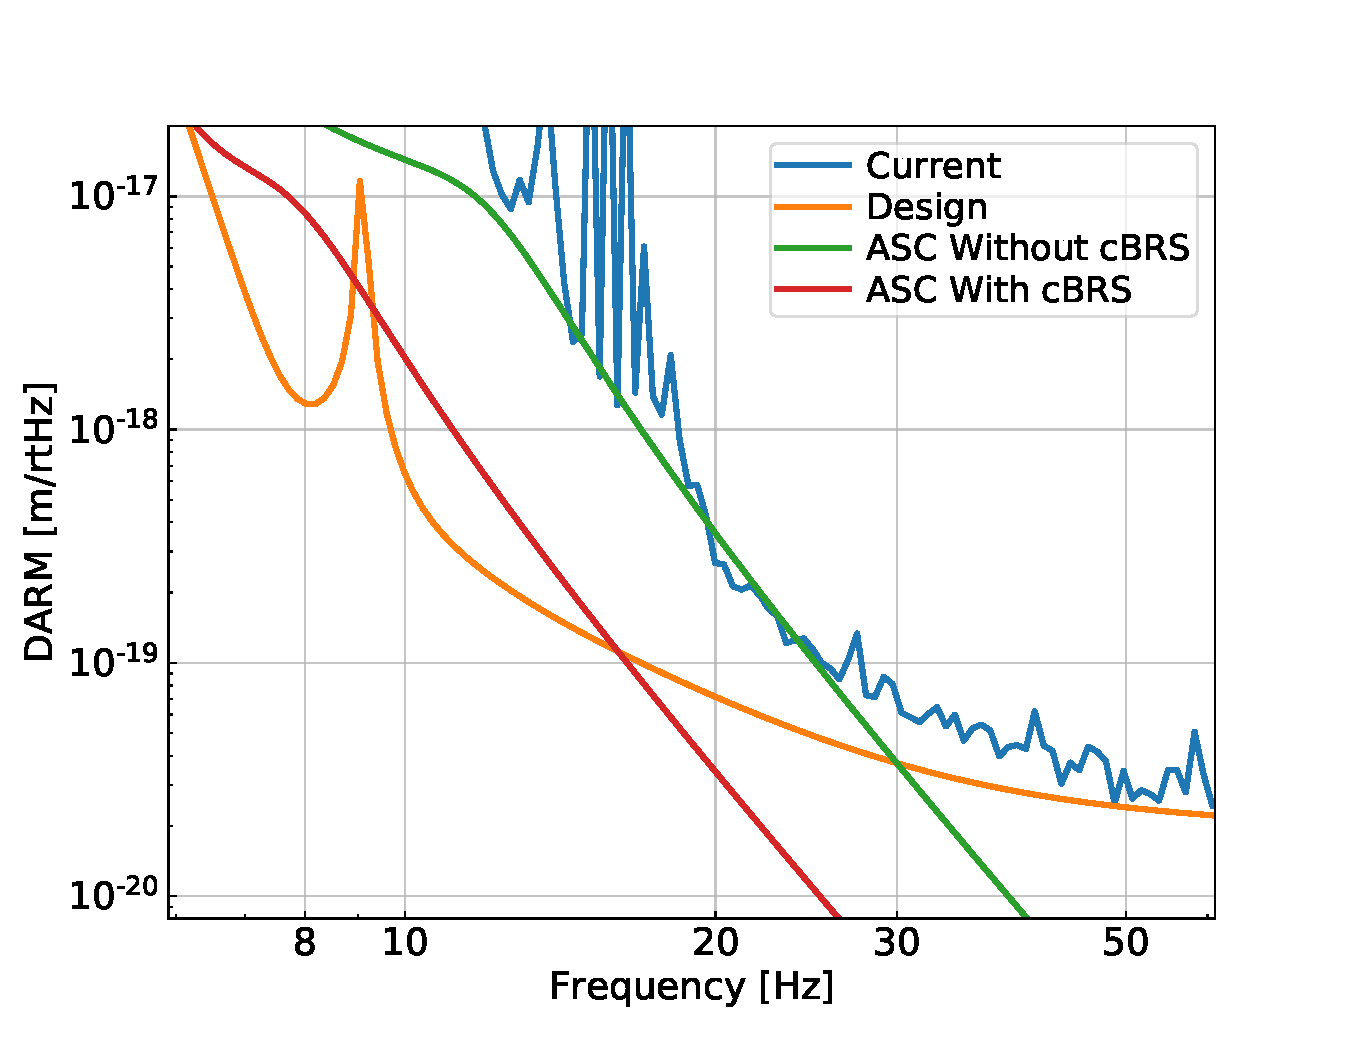
\includegraphics[width=\textwidth]{cBRS_ASC.pdf}
\caption[Projected low frequency strain noise with and without the cBRS]{Projected low frequency strain noise with and without the cBRS. The blue line is the current sensitivity of LLO, the orange is the aLIGO design sensitivity, green is the modeled noise contribution of the current ASC system, and red is the improved ASC noise contribution with the seismic isolation described in Section \ref{IsoScheme}. }
\label{ascStrain}
\end{center}
\end{figure}

\chapter{Auxiliary Applications}
\quad With every novel sensor comes novel science. Thus the development of these highly sensitive rotation sensors have opened up a handful of novel scientific avenues, tangential to seismic isolation, that have been explored.

\section{Geophysics}
Seismic waves have six components, three translations and three rotations, however seismology has long neglected the rotational components due the lack of sensitive rotation sensors. Recent developments have begun to alleviated this issue with the advent of seismically relevant ring laser gyros. \cite{ring} The rotation sensors described in Chapter \ref{BRS_chap} and \ref{cBRS_chap} join a small class of ground rotation sensors that are sensitive at low frequencies and have low translational coupling which allow for the use in seismology.
\subsection{Rayleigh Wave Theory}

Seismic waves can be broken into two classes: body waves and surface waves. In regard to surface waves there are two polarization: Love waves and Rayleigh waves. The motion caused by a Love wave is constrained to the plane parallel with the surface of the medium while Rayleigh waves are constrained to a plane perpendicular the surface. 

The plane wave solution of a Rayleigh wave has six components ($u_x, u_y, u_z, \theta_x, \theta_y, \theta_z$) where $u_i$ designated the translational motion in the $i$th direction while $\theta_i$ is the rotation about the $i$th axis.
These can be described as with the following \cite{seismic}
\begin{align}
u_x({\bf r} ,t)&=\alpha \sin(\zeta) \cos(\phi) \cos(\omega t-{\bf k}\cdot{\bf r})\label{XEq}\\
u_y({\bf r} ,t)&=\alpha \sin(\zeta) \sin(\phi) \cos(\omega t-{\bf k}\cdot{\bf r})\\
u_z({\bf r} ,t)&=\alpha \cos(\zeta) \cos(\omega t-{\bf k}\cdot{\bf r}+\pi/2)\label{ZEq}\\
\notag \\
\theta_x({\bf r} ,t)&=\frac{\partial u_z}{\partial y}=\alpha \kappa \cos(\zeta) \sin(\phi) \cos(\omega t-{\bf k}\cdot{\bf r})\label{TiltXEq}\\
\theta_y({\bf r} ,t)&=-\frac{\partial u_z}{\partial x}=-\alpha \kappa \cos(\zeta) \cos(\phi) \cos(\omega t-{\bf k}\cdot{\bf r})\\
\theta_z({\bf r} ,t)&=\frac{1}{2}\Big(\frac{\partial u_y}{\partial x}-\frac{\partial u_x}{\partial y}\Big)=0
\end{align}

where $\alpha$ is the amplitude, $\zeta$ is the ellipticity angle, $\phi$ is the angle of incidence in the horizontal plane, $\omega$ is the frequency, and $\bf{k}=\kappa (\cos(\phi),\sin(\phi),\text{0})$ is the wavevector.

These components can be seen in Figure \ref{Earthquake} which shows the seismic waves sourced by a M 7.9 earthquake in Papua New Guinea as seen by instruments installed at the End-Y station of the LIGO Hanford Observatory (LHO). The translations were measured by a broadband three-component seismometer while the rotation was sensed by a Beam Rotation Sensor (BRS) described in Chapter \ref{BRS_chap}. As one would expect from Eq. \ref{ZEq} and \ref{TiltXEq}, the vertical velocity and the rotation differ only by a constant factor related to the phase velocity and the angle of incidence. Additionally, a large amplitude Love wave is apparent starting at $\sim$1200 seconds which neither the vertical seismometer or the BRS experiences due to the waves' lack of vertical component.

\begin{figure}%
\begin{center}
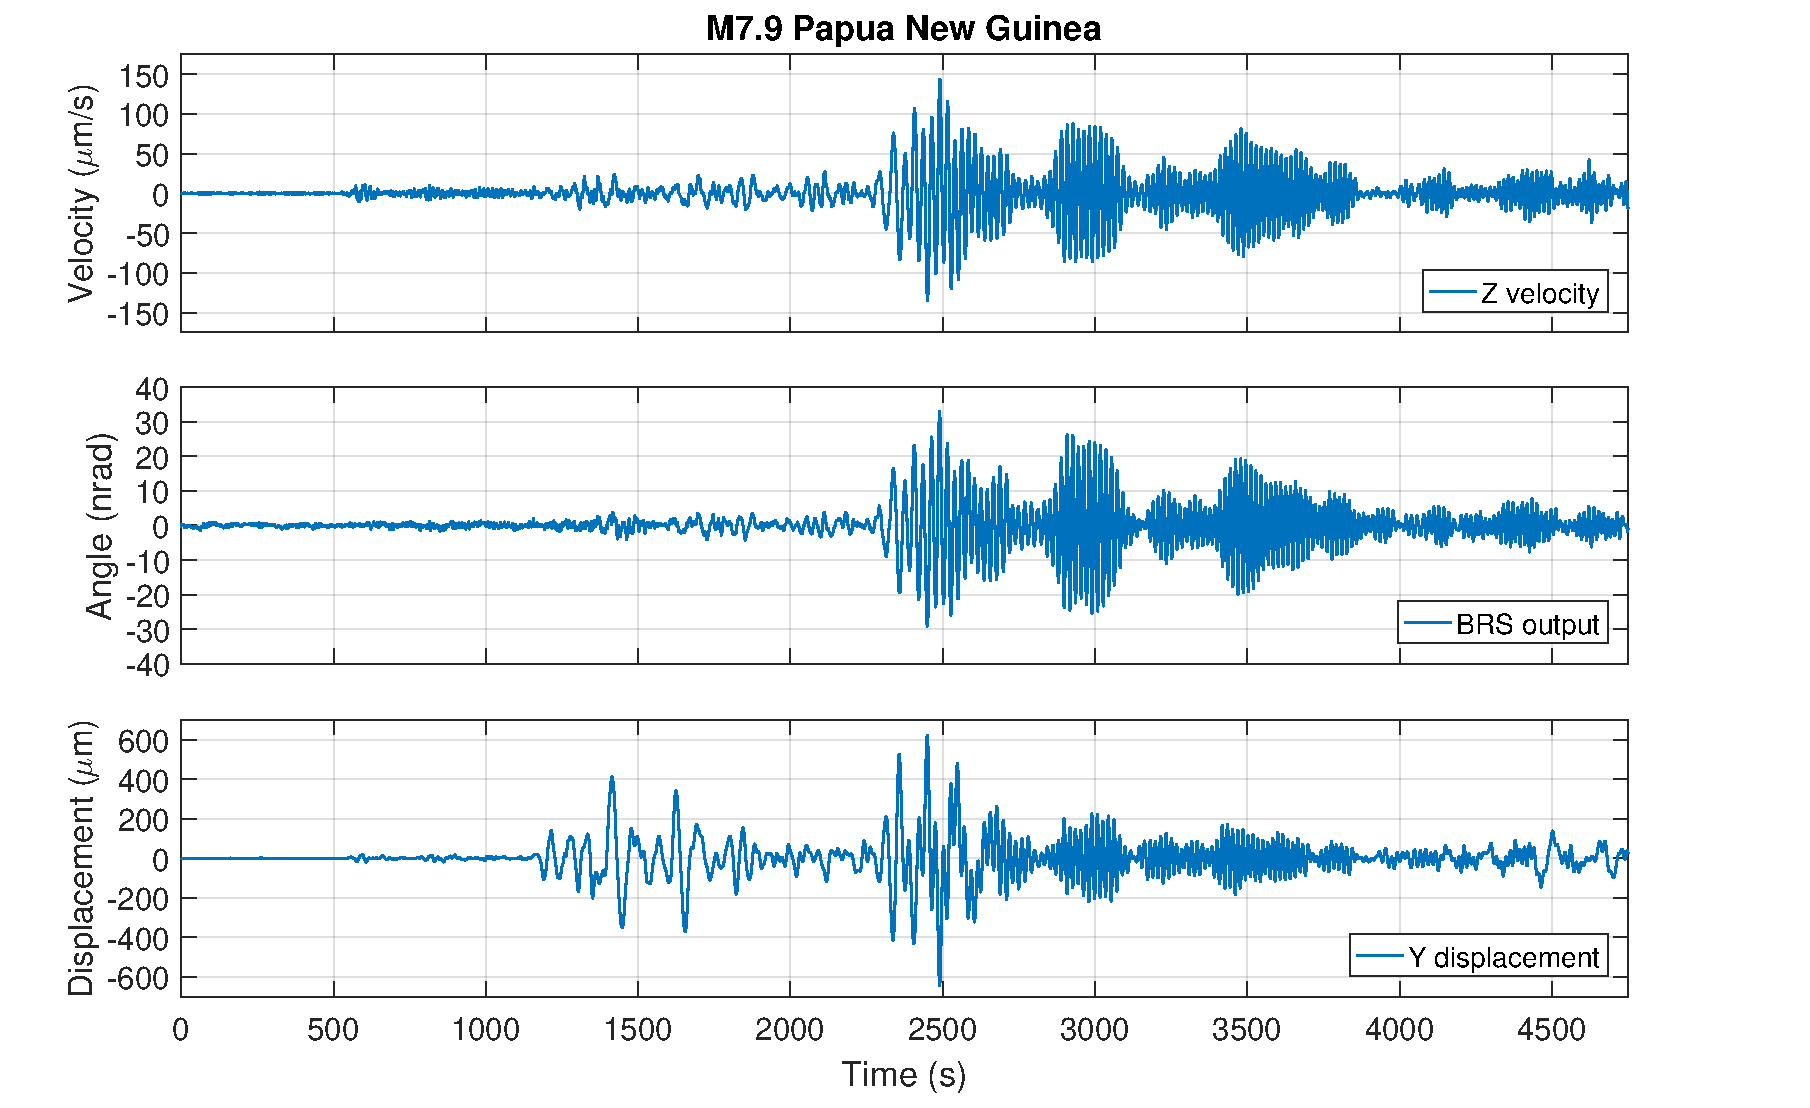
\includegraphics[width=\textwidth]{PNGTimeSeries.pdf}
\caption[Observations of the seismic waves by instruments installed at the End-Y Station of LHO]{Observations of the seismic waves emanated from a M7.9 earthquake in Papua New Guinea as seen by instruments installed at the End-Y Station of LHO. \cite{tiltSeismology} Both the Z velocity and Y displacement were measured by a broadband three-component seismometer while the rotation was measured by a BRS described in Chapter \ref{BRS_chap}. }
\label{Earthquake}
\end{center}
\end{figure}

From Equations \ref{XEq}-\ref{ZEq} it can be seen that with only a traditional 3-axis seismometer, it is impossible to measure all five parameters that define this wave-field. \footnote{With an array of vertical seismometer four parameters: frequency, angle of incidence, wavenumber, and amplitude, can be readily measured.}Additionally, the horizontal components, $u_x\text{ and }u_y$ can contain contributions from co-propagating Love waves which further muddles ones ability to extract parameters. 


\subsection{Wave-Field Parameter Extraction}

With the combined measurements of the translational and rotational components at a single station, one can extract wavefield parameters that would otherwise be difficult to obtain, namely the phase velocity and angle of incidence. 

Seismic wave phase velocities are common observables which not only allows for understanding of Rayleigh wave propogation but can be inverted to yield tomographical structure profiles of the interior of the earth. \cite{tomography} The traditional method of extracting these is by exploiting the time of arrival of a wave as it passes through an array of many seismometers. The analysis can be constrained to only the vertical channel as it is insensitive to Love waves which could contaminate the measurements. However, this method requires many devices and effectively averages over the size of the array.

Alternatively, with measurements of the rotational components, a point-like measurement of the phase velocity can be made with three devices, a 3-component seismometer and two horizontal rotation sensors. This can be shown in the following equations:
\begin{align} 
v&\equiv\frac{\omega}{\kappa} = \frac{\dot{u_z}}{\theta_x}\sin(\phi) \label{vx} \\
v&=\frac{\dot{u_z}}{\theta_y}\cos(\phi)\label{vy} \\
v&=\frac{\dot{u_z}}{\sqrt{\theta_x^2+\theta_y^2}} \label{v}
\end{align}

where the dot represents the temporal derivative. Equations \ref{vx} and \ref{vy} can be utilized if a station has only one horizontal rotation sensor but requires independent determination of $\phi$, the angle of incidence. In contrast, Equation \ref{v} contains only information from a single station.

In addition to the phase velocity, the angle of incidence can be determined with the following:
\begin{align}
\phi=\text{arctan}\bigg(\frac{\theta_x}{\theta_y}\bigg)
\end{align}

Although in theory, this can be measured using a single seismometer, Love wave contamination of the horizontal translational channels would distort any such measurement. As the horizontal rotational channels are insensitive to Love waves, they allow the extraction of $\phi$ without such contamination.  

\subsection{Single Station Dispersion Measurements}
%\subsubsection{Hanford Measurements}
As described in Section \ref{BRS_Hanford}, two BRSs were installed at LHO, one at each end station located 5.66 meters apart. The End-X BRS was found to have a $\delta=30\ \mu \text{m}$ leading to a translational coupling of $2 \times 10^{-4}$ rad/m while the End-Y BRS was found to have a coupling of $1 \times 10^{-6}$ rad/m with a $\delta<0.5\ \mu \text{m}$. This limited any seismic studies using these devices to use only the End-Y BRS as the End-X BRS was contaminated with translational motion. 

Between April, 2016 and January, 2017, six earthquakes were measured during environmentally quite times at the observatory. \cite{tiltSeismology} With application of Equation \ref{vx} the phase dispersion curve at the End-Y Station was measured with instruments installed at a single station. Corrections of the angle of incidence were determined by an array of seismometers installed at LHO which were verified via great circle calculations. Additionally, the phase velocity was estimated in a more traditional manor using the signal delay between the array of seismometer at LHO. The measure phase dispersion curve is shown in Figure \ref{Phase_Hanford} which shows good agreement between the two methods. For more detail see Reference \cite{tiltSeismology}
 
\begin{figure}%
\begin{center}
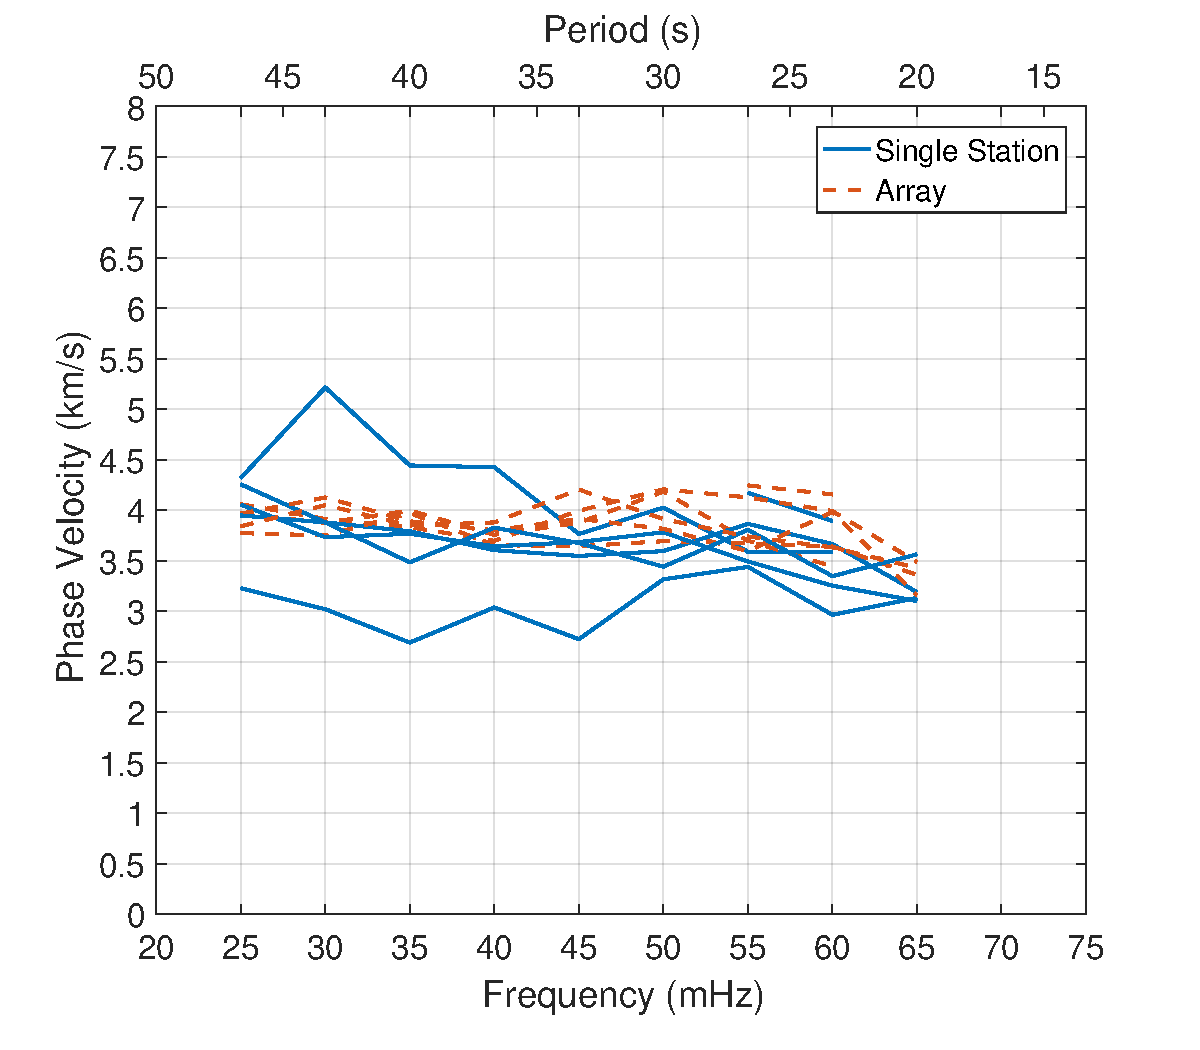
\includegraphics[width=0.75\textwidth]{Vel.pdf}
\caption[Single station Rayleigh wave phase velocity measurements]{Rayleigh wave phase velocity measurements made by instruments located at the End-Y station of LHO, blue, and the same measurements achieved by the array of seismometers deployed at LHO. Each line represent the measurements achieved by different earthquakes. The angle of incidence of each wave was measured independent of the single station and used within the analysis. \cite{tiltSeismology}}
\label{Phase_Hanford}
\end{center}
\end{figure}

These measurements display the utility of including rotation sensors in seismic instruments. If a seismic station was constructed with two orthogonally oriented horizontal rotation sensors and a vertical seismometer, the phase velocity could be measured independent of angle of incidence by utilizing Eq. \ref{v}. Neglecting the logistical difficulty, one could imagine constructing arrays of station with both translational and rotational sensors. This would allow mapping of the phase dispersion curves, and thus tomography, with spatial resolution limited only by the size of the instruments. Such stations could also be installed within traditional arrays to yield independent point-like measurements to further constrain tomographic studies.

%\subsubsection{Livingston Measurements}
%
%\begin{figure}%
%\begin{center}
%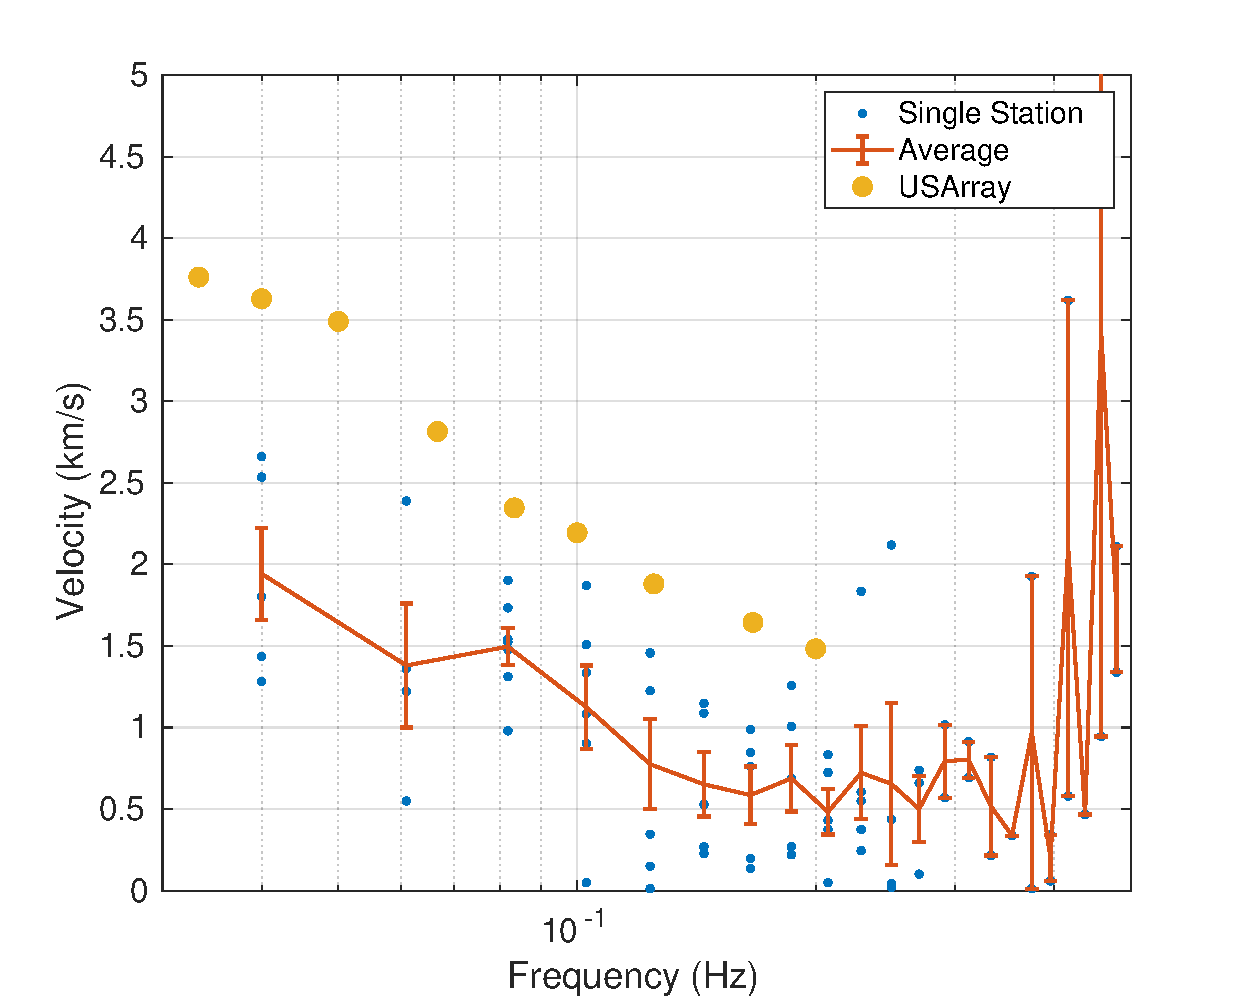
\includegraphics[width=\textwidth]{RayleighDispersion.pdf}
%\caption{True single station Rayleigh wave phase velocity measurements achieved at LLO. The measurements from each earthquake are shown in blue while red shows the average and standard deviation of these measurements. The yellow dots represent measurements made independently by the USArray seismometer array deployment.}
%\label{Phase_Livingston}
%\end{center}
%\end{figure}

\section{Newtonian Noise}
\subsection{Theory}

The gravitational coupling between the environment and an interferometer's test masses, so called Newtonian noise, is expected to limit the performance of terrestrial gravitational wave detectors in the near future \cite{Saulson}. Sources of the gravitaitonal field variations can range from atmospheric density changes to vibrations of the laboratory structures \cite{terrestrial}. This coupling is unique in the fact that it can not be shielded or trivially engineered away. One can move an observatory underground to decrease the strength of the atmospherically driven fluctuations and those caused by seismic surface waves, discussed in detail in the following section. However, this process is both expensive and does not remove the sources which come from operating an instrument such as the vibrations of the vacuum structure or seismic motion sourced by laboratory equipment. 

For the current surface-level interferometric observatories, the seismic motion due to Rayleigh waves is thought to be the dominant contributor to the Newtonian noise and will be the limiting noise source between 8-20 Hz \cite{NN2}. The motion due to a plane Rayleigh wave follows:

\begin{equation}
u_z({\bf r} ,t)=u_z \cos(\omega t-{\bf k}\cdot{\bf r}+\pi/2) \label{uz}
\end{equation}

where $u_z=\alpha \cos(\zeta)$, $\alpha$ is the amplitude, $\zeta$ is the ellipticity angle, $\phi$ is the angle of incidence in the horizontal plane, $\omega$ is the frequency, and $\bf{k}=\kappa (\cos(\phi),\sin(\phi),\text{0})$ is the wavevector. The corresponding test mass acceleration in the x-direction follows \cite{Harms_2016}:
\begin{equation}
a_x({\bf r} ,t)=2 \pi u_z \gamma G \rho_0 e^{-h \kappa}  \cos(\phi) \cos(\omega t-{\bf k}\cdot{\bf r}) \label{a}
\end{equation}
where $G$ is the gravitational constant, $\rho_0$ is the density of the ground, $h$ is the height of the test mass from the ground, and $\gamma \approx 0.8$ is a factor which accounts for the counter-action of the change of density due to the seismic wave and the vertical motion of the ground.

At first glance, these equations appear to suggest that one could predict the test mass acceleration for a given vertical seismometer signal. Such a prediction would allow for high quality subtraction of the Newtonian Noise from an observatory's data stream. However, true seismic wave-fields are not composed of stationary Rayleigh waves but instead are comprised of the sum of many desperate sources which may change their amplitude and phase in time. With this consideration, the phase difference between Eq. \ref{uz} and \ref{a} and the lack of angle of incidence dependence in Eq. \ref{uz} destroy the ability to use a single vertical seismometer as a reliable sensor for Newtonian noise subtraction.

On the other hand, a horizontal seismometer described by Eq. \ref{XEq} is both in-phase with the Newtonian noise signal and has the same angular dependence. However, seismic wave-fields also include Love waves which have horizontal components but no vertical. This contaminates these channels and would decrease the correlation between the horizontal seismometer and the Newtonian noise. 

Finally, the tilt, being the rotation about the y-axis, due to a Rayleigh wave is described by the following:

\begin{equation}
\theta_y({\bf r} ,t)=\frac{\partial u_z}{\partial x}=u_z \kappa \cos(\phi) \cos(\omega t-{\bf k}\cdot{\bf r})\label{tX}\\
\end{equation}

The tilt is thus both in-phase, has the same angular dependence, and does not include Love waves. The lack of Love waves can be seen in Figure \ref{Earthquake} when the horizontal seismometer experiences a large Love wave at around 1200 s while the rotation sensor sees no such signal. The tilt signal and the Newtonian noise are thus related by a handful of parameters which can be measured independently or determined empirically and are not expected to vary in time. This points to the conclusion that a tiltmeter is the ideal sensor for Newtonian noise subtraction

\subsection{Observations}

During LIGO's second observing run (O2), a prototype cBRS, described in Chapter \ref{cBRS_chap}, was installed at the corner station of the LIGO Hanford Observatory along side an array of vertical seismometers. The aim of this deployment was to investigate the Newtonian noise coupling and to test subtraction schemes. Ideally, one would place a rotation sensor directly below one of the test mass as the Newtonian noise acting on the mirror is dominated by the ground just beneath it. However, the cBRS was too large to be placed underneath the vacuum chamber which holds the test mass so it was placed just next to the vacuum chamber as can be seen in Figure \ref{NNArray}.

\begin{figure}[!h]
\begin{center}
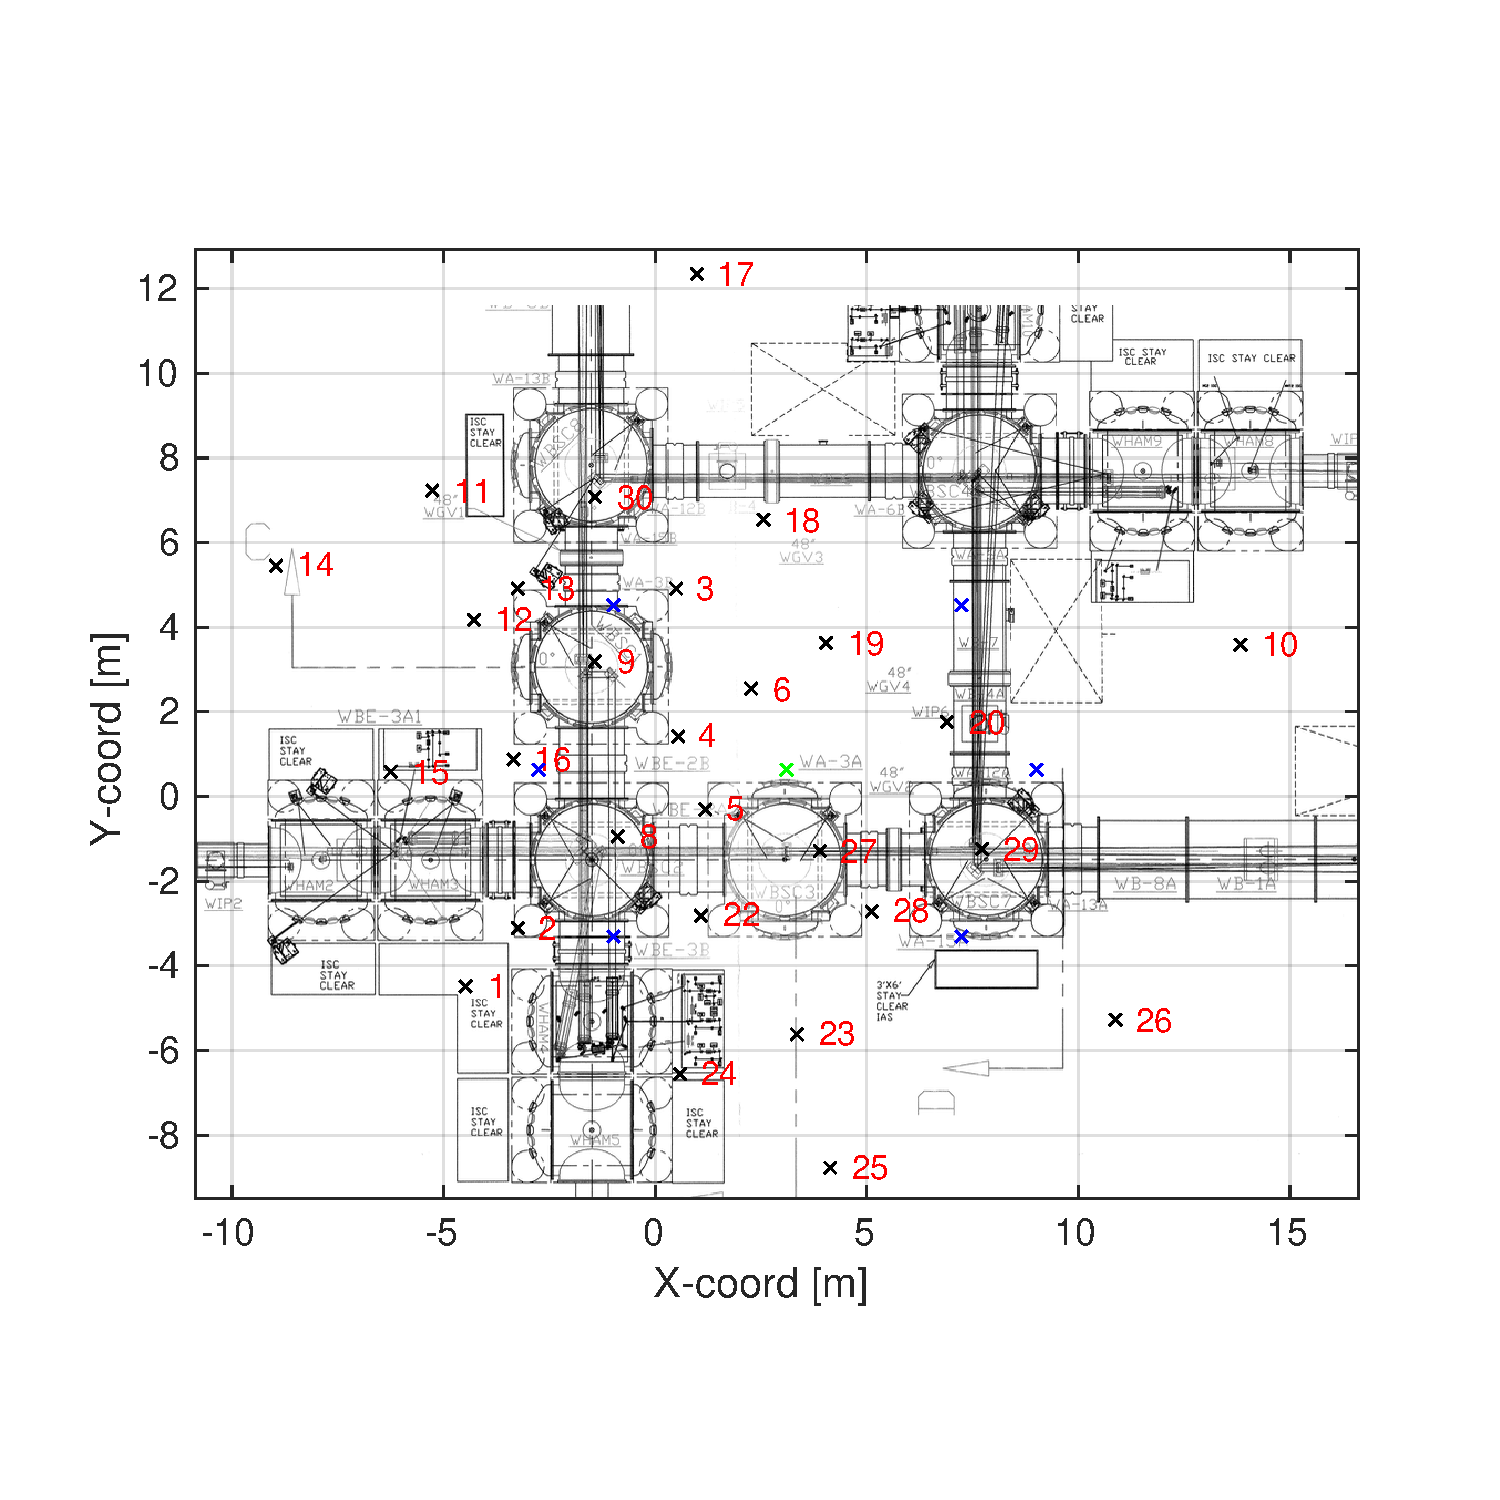
\includegraphics[width=\textwidth]{NNArray.pdf}
\end{center}
\caption[The location of the cBRS during O2 alongside the array of seismometers]{The location of the cBRS , marked by the green $\times$, during O2 alongside the array of seismometers, marked by the black $\times$s, overlaid on a schematic of the LHO corner station vacuum chambers.}
\label{NNArray}
\end{figure}

The first goal of this instrumentation deployment was to assess the ability to combine an array of vertical seismometers to significantly subtract Newtonian noise. Unfortunately, the observatory was not sensitive enough to observe Newtonian noise with high signal-to-noise. Thus the cBRS was used as a proxy for the signal that would be seen by a future observatory. In order to achieve the combination of the 30 seismometer signals which optimally approximates the cBRS signal, a Weiner filter was constructed using seismometers as the references and the cBRS as the target. 

The results of this subtraction can be seen in Figure \ref{NNSub} \cite{NN} which shows that a single seismometer can achieve a factor of $\sim$1.5 reduction while the combination of all 30 seismometers achieves a reduction of $\sim$10. This can be understood with Equations \ref{uz}-\ref{tX}. The signal from a single vertical seismometer will not have the angular dependence or phase as the tilt. However, the collection of seismometers can simulate the tilt by combining pairs of seismometers to act as effective rotation sensors.

These observations have shown that an array of 30 vertical seismometers can be expected to yield Newtonian noise reduction for future observatories of at least an order of magnitude. Indeed, similar subtraction was achieved when only the best five seismometers were included as reference channels. This points to the possibility of smaller well placed arrays also achieving similar reduction.

\begin{figure}[!h]
\begin{center}
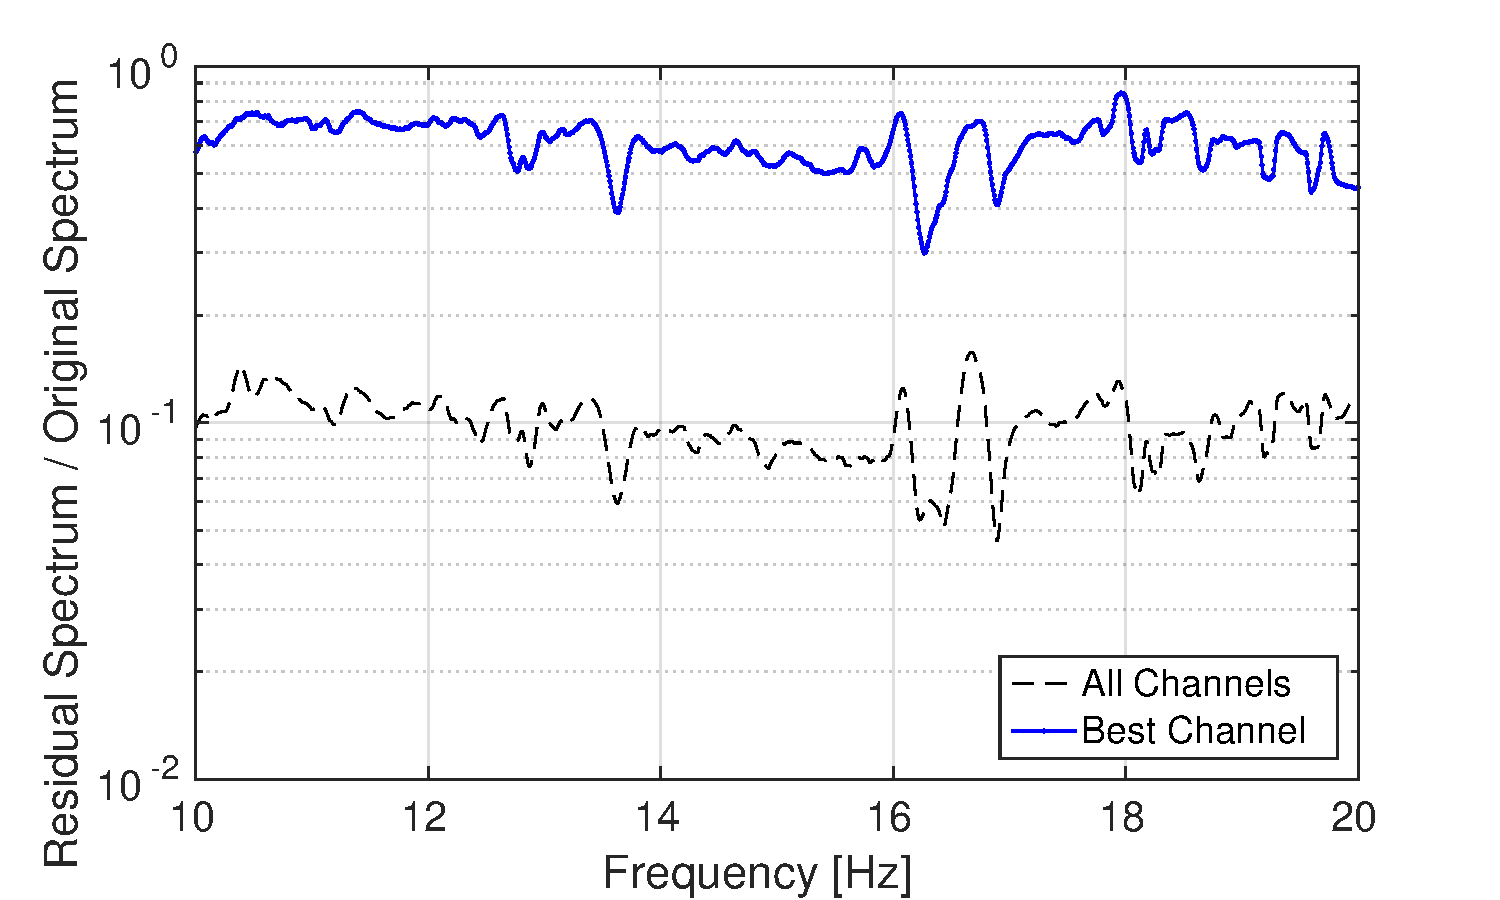
\includegraphics[width=0.75\textwidth]{NNSubtraction.pdf}
\end{center}
\caption[Projected Newtonian noise subtraction with the array of seismometers]{Projected Newtonian noise subtraction with the array of seismometers using the cBRS as a proxy for the noise that would be seen by a future observatory.}
\label{NNSub}
\end{figure}

The second goal of this array was to investigate the coupling between ground tilt and strain for the observatory during O2. This was achieved by calculating the transfer function between the cBRS output and strain using a month of data. The resultant transfer function is shown in Figure \ref{NNCoupling} where it is apparent coupling is observed across many frequencies with a single-to-noise of $\sim$10-30. The noise was estimated by recalculating the transfer function with the two data streams shifted relative to one another by 1000 s. 

\begin{figure}[!h]
\begin{center}
\includegraphics[width=0.75\textwidth]{NNCoupling.pdf}
\end{center}
\caption[Transfer function between the cBRS and the strain output of the interferometer]{Transfer function between the cBRS and the strain output of the interferometer alongside various non-gravitational coupling mechanisms and a model for the Newtonian noise caused by an isotropic, homogeneous Rayleigh wave-field.}
\label{NNCoupling}
\end{figure}

The nature of this coupling can not be known to be of gravitational nature a piori. Thus a collection of possible non-gravitational coupling mechanisms were investigated. \cite{NN} Namely, seismic coupling through the seismic isolation system. This path follows from ground tilt to suspension point motion which propagates to the test mass. The transfer function from the ground tilt to suspension point motion can be readily measured using the sensors on the isolation platforms. This was then propagated to test mass motion using an analytical model of the suspension, Sus L, and a previously measured transfer function from suspension point to test mass, Sus L/P, which includes both the length and pitch couplings.

These first observations pointed to the possibility that the current observatories are already being affected by Newtonian noise. However, further modeling and investigation \cite{NN2} found that the distinction between gravitational and non-gravitational coupling is still ambiguous. Deployment of future instruments, including a rotation sensor designed specifically to observe Newtonian noise, should disentangle these couplings and may allow for the first subtraction of Newtonian noise from strain output of the interferometer.

\printendnotes
\nocite{*}   
\bibliographystyle{unsrt}
\bibliography{Dissertation}
\end{document}


